\section{Analysis of calibration files}
\protect\label{section:analysiscalib}

\textit{I wonder if this section should be considerably condensed at it doen't
contribute too much except to show all the blind alleys I've been up, the later
work on bad pixels is much more promising for eliminating the bulk of the
negative pixels and I can use more of the daily flats. I think I need to
explain why I think the master bias and flat files don't cut it and the efforts
made to replace them and also keep track of the error bars on them.}

The initial display of images and preliminary results shown above raise
questions about the calibration files used, so some effort was undertaken to
study these and perhaps make adjustments.

\subsection{Analysis of bias files}
\protect\label{section:biasanal}

Two sample sets of master bias files are illustrated in Fig. \ref{fig:mastbeg0918} and Fig.
\ref{fig:mastbeg0120}, either side of the change to the areas and starting
positions on the CCD in March 2019.

\begin{figure}[!htbp]
\begin{center}
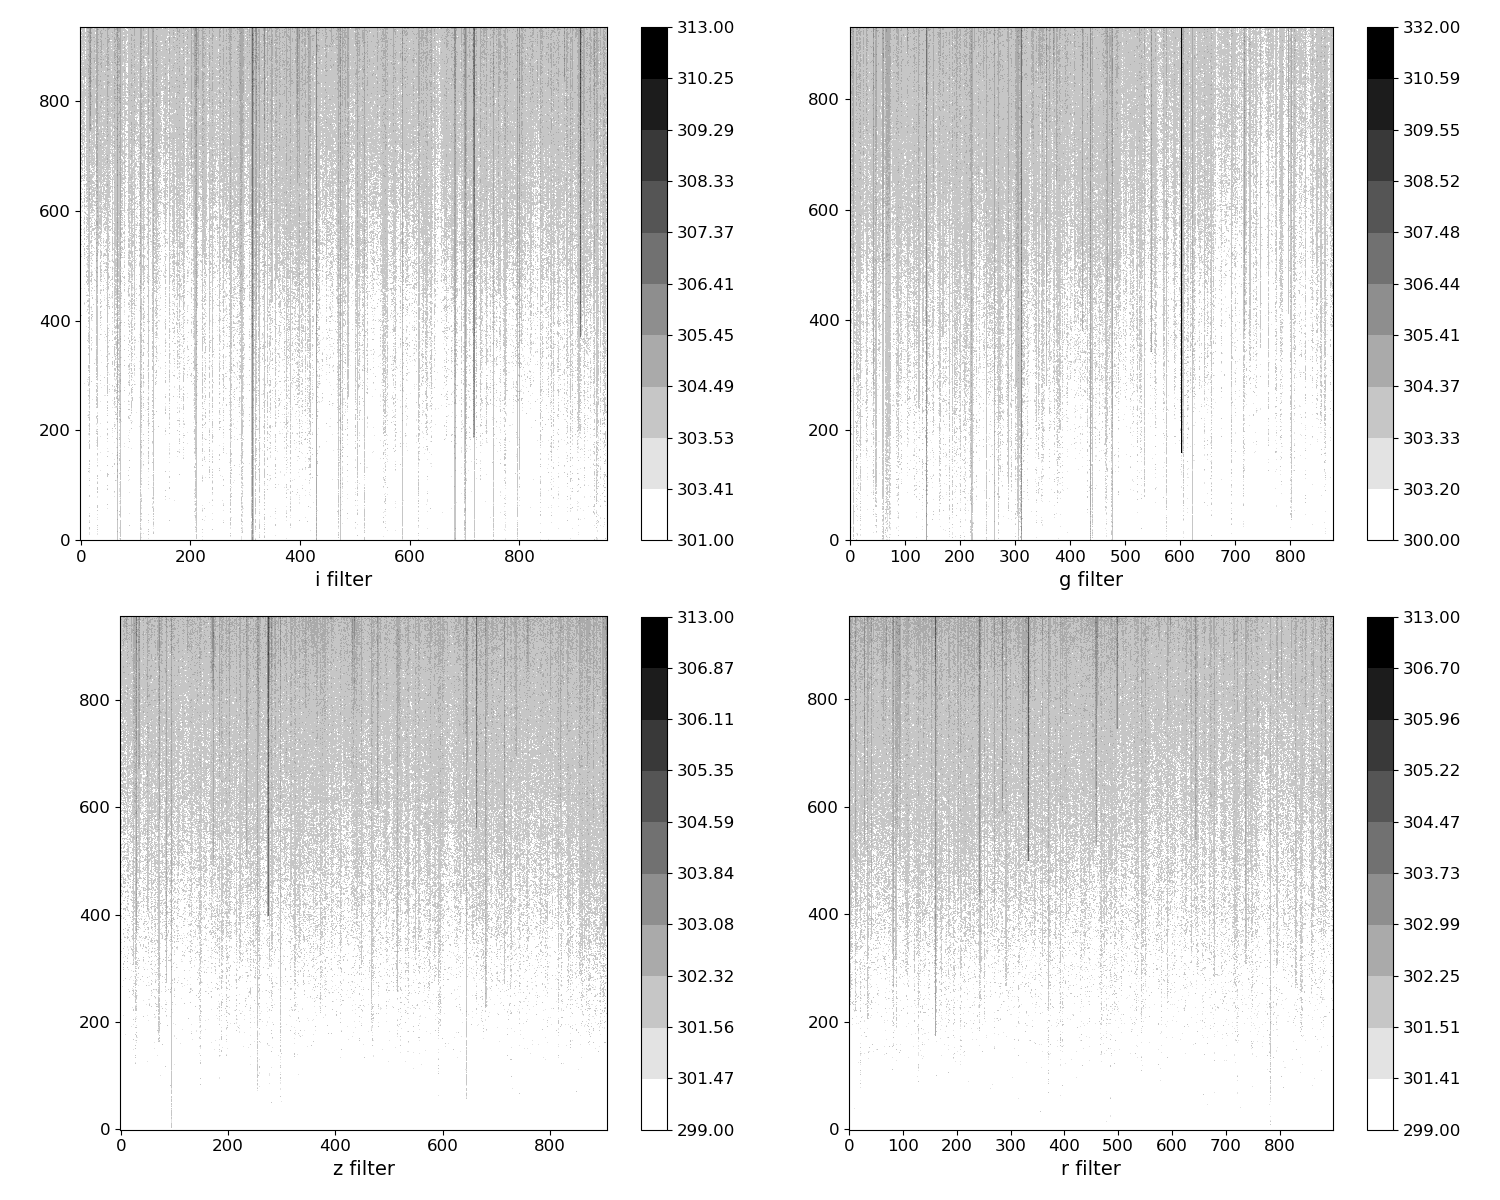
\includegraphics[scale=0.4]{images/mastbiaseg0918.png}
\end{center}   
\caption{This illustrates the 4 master bias files (provided for September
2018) for each filter used to construct Fig. \ref{fig:initgexample} and Fig.
\ref{fig:init4example}. The positions of the 4 images reflect the positions and orientations in which the
images are taken from the CCD.}
\protect\label{fig:mastbeg0918}
\end{figure}

\begin{figure}[!htbp]
\begin{center}
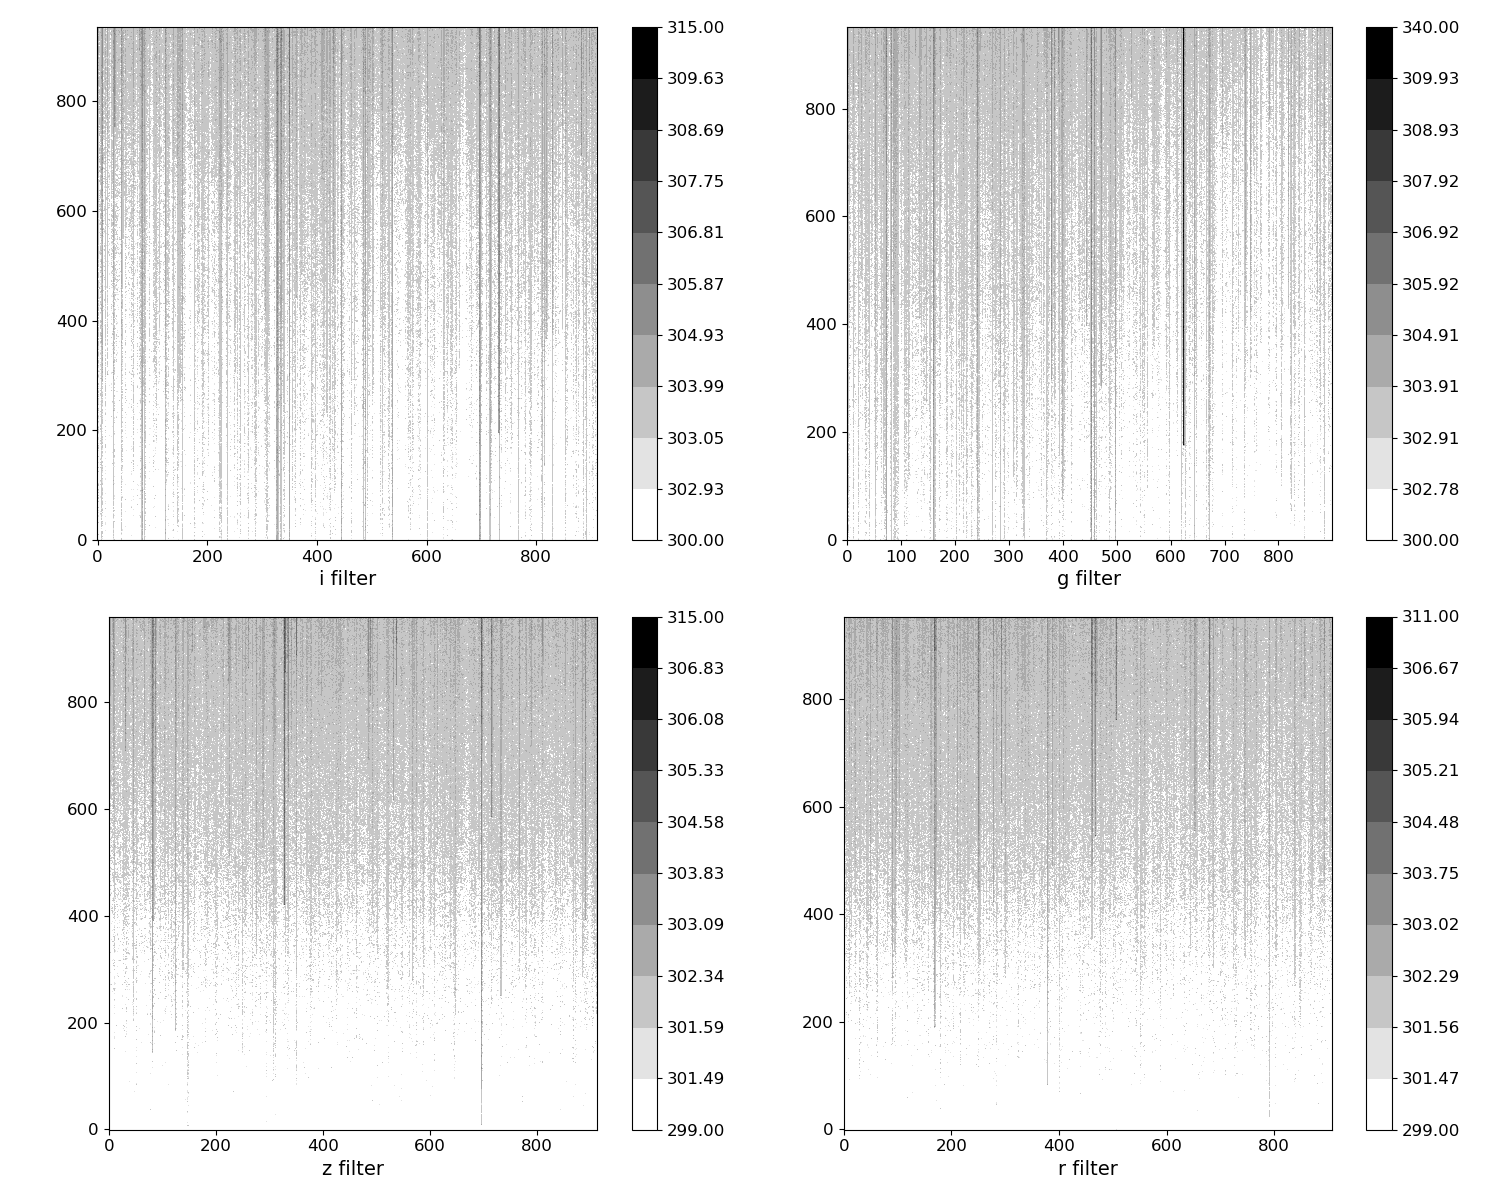
\includegraphics[scale=0.4]{images/mastbiaseg0120.png}
\end{center}   
\caption{This illustrates the 4 master bias files for each filter for January
2020, for comparison with Fig. \ref{fig:mastbeg0918}. The differences are due
to changes in the area and starting positions on the CCD for images made in
March 2019.}
\protect\label{fig:mastbeg0120}
\end{figure}

A study was made of the bias files to ascertain the level of the bias current
and assess the noise. Of particular concern was that subtraction of the bias
from observation files, in all cases, not just the most noisy bias files, yielded
negative pixel results from all the observation files, particularly those from
the \texttt{g} and \texttt{z} filters, for example, taking the
observations and master bias files for 5  September 2018, the total negative values shown in 
Table \ref{table:negmast} are observed.

\begin{table}[!htbp]
\begin{center}
\begin{tabular}{lrr} \hline
Filter & Min & \% negative \\\hline
g & -27 & 28.90 \\
i & -20 & 5.42 \\
r & -19 & 5.52 \\
z & -20 & 9.90 \\
\hline
\end{tabular}
\end{center}
\caption{Negative values of pixels in image minus monthly master bias for
various filters on 5 September 2018, for all observations of \bstar, through
various visible light filters}.
\protect\label{table:negmast}
\end{table}

This was also found in the daily flat files, although it proved possible to
eliminate them by careful choice of the daily  flat files as described in
Section \ref{seciion:altmasters}.

The location of the negative pixels is distributed quite widely across the
images, there is no restriction to a handful of places which could be identified
as bad pixels and made into a mask. This can be demonstrated by examining
observation files, subtracting the relevant master bias file for the month and
counting where each pixel goes negative. The result can be seen in Fig.
\ref{fig:negpixloc}. It will be clear that pixels can become negative all over
the images, but the edges of the images from some of the filters, for example
the bottom edge of the \texttt{g} filter and the right edge of the \texttt{z}
filter are especially bad.

\begin{figure}[!htbp]
\begin{center}
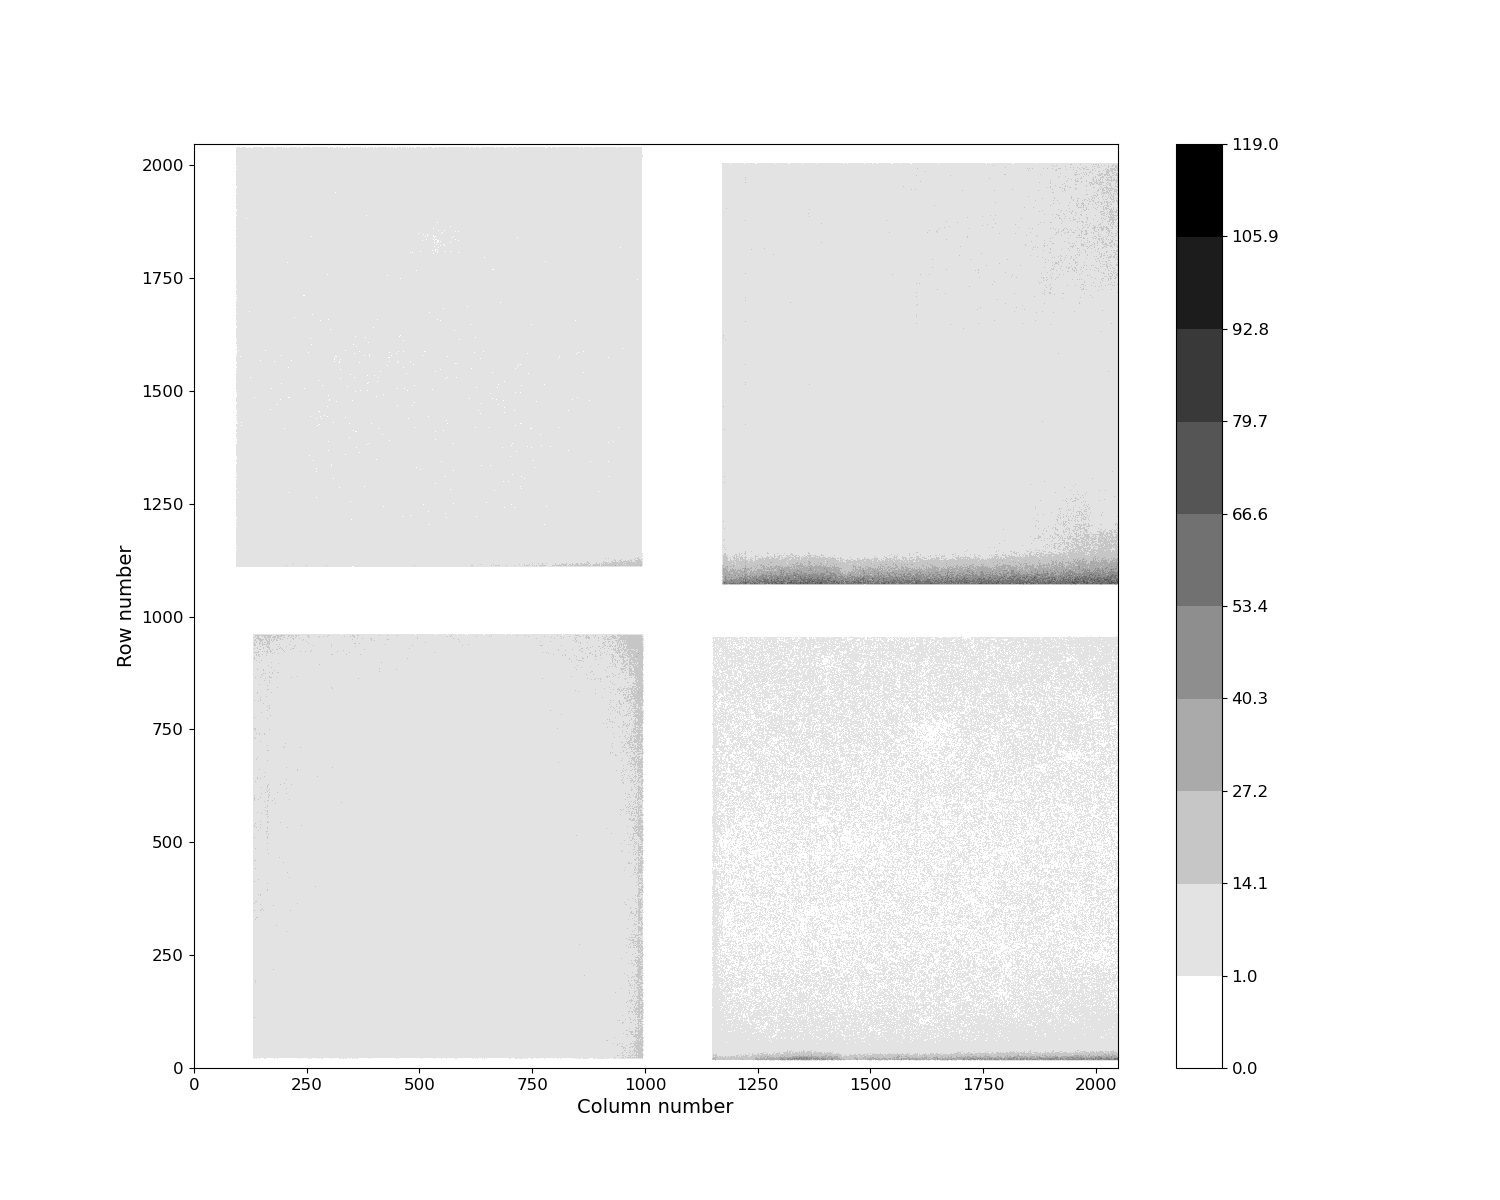
\includegraphics[scale=0.4]{images/min200negpix.png}
\end{center}   
\caption{This shows a representation of the entire CCD array and
analysing all the observations (omitting those with minimum values less than
200 counts or greater than 61,000 counts in one or more pixels) for each of the
visible light filters, counting each time the corresponding pixel goes negative
after subtraction the corresponding bias files. It may be helpful to compare this with Fig.
\ref{fig:showusedccd} to show the portions of the CCD used.}
\protect\label{fig:negpixloc}
\end{figure}

\subsubsection{Master bias files}
\protect\label{section:masterbiasfiles}

In Fig. \ref{fig:mastmeanbias} is shown the mean value and standard deviation of
the master bias files up to March 2020.

\begin{figure}[!htbp]
\begin{center}
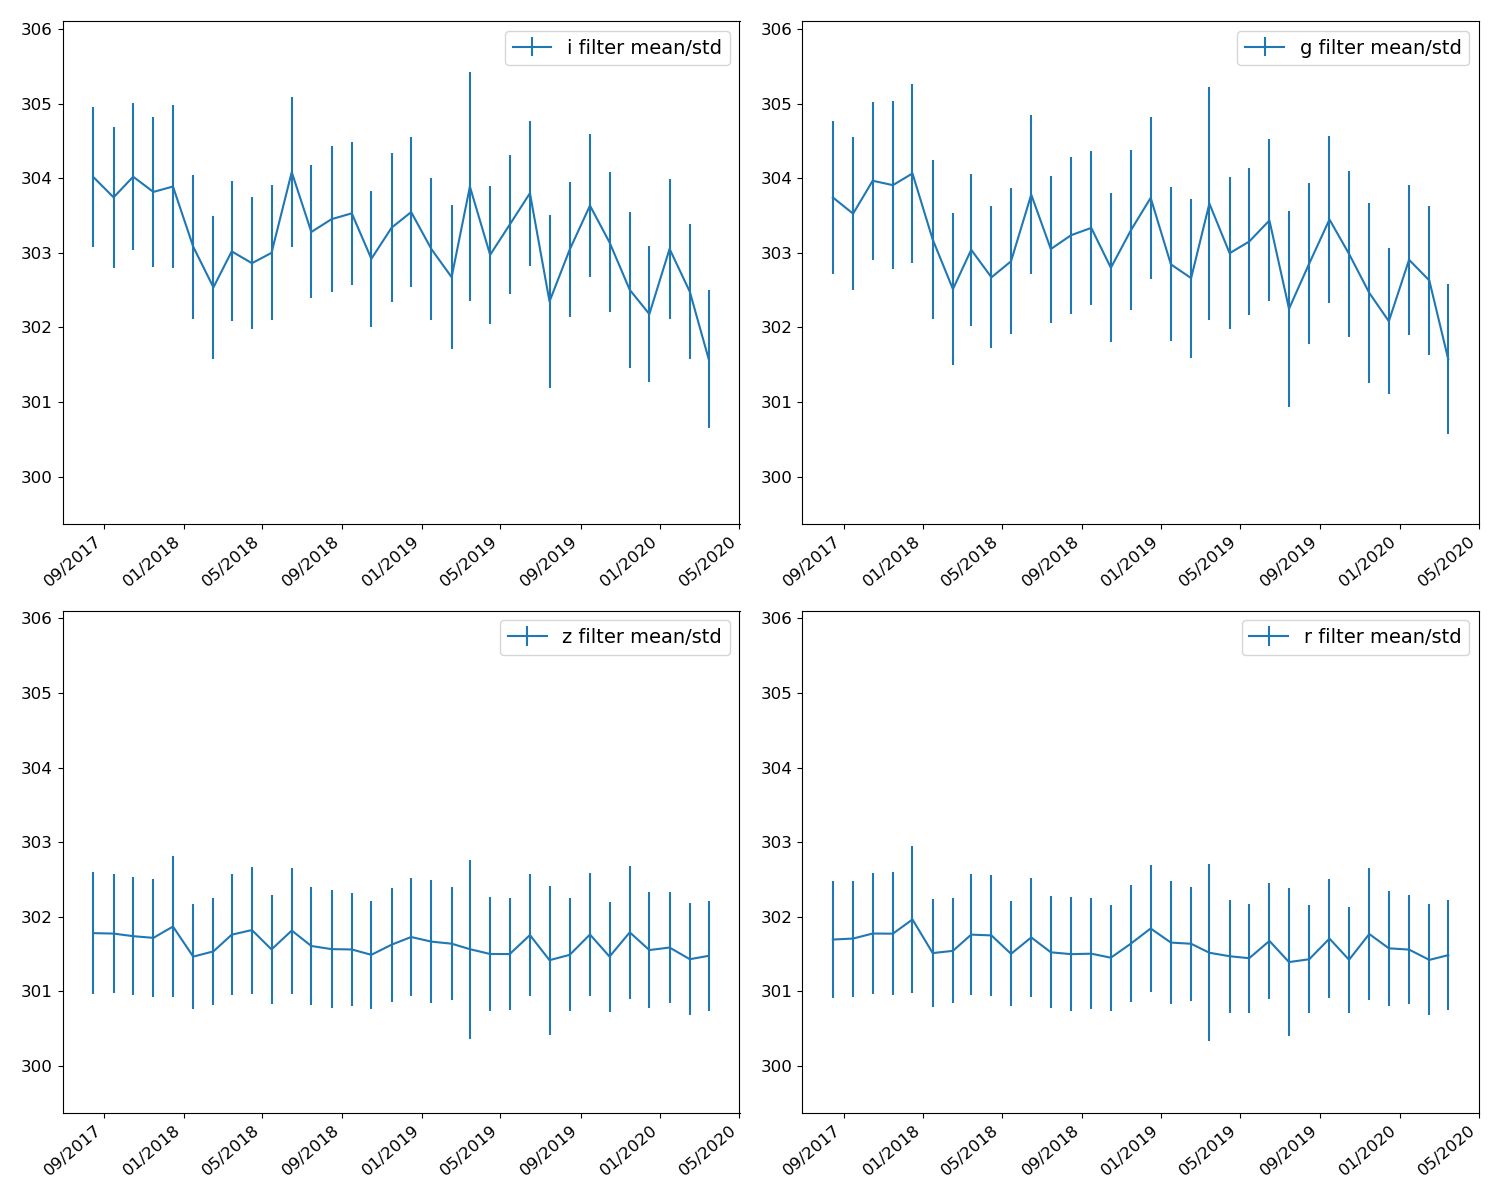
\includegraphics[scale=0.4]{images/mastmeanbias.png}
\end{center}   
\caption{This illustrates the mean and the standard deviation of the values in
the master bias files from July 2017, when {\rdwarf} targets were first
observed, until March 2020.}
\protect\label{fig:mastmeanbias}
\end{figure}
\clearpage

The master bias files are constructed from the daily bias files for the
corresponding month for each filter as follows:

\begin{enumerate}
  \item Tabulate the mean and standard deviation of each pixel count in each
  bias file.
  \item Take the median mean (\textit{med\_e}) and the median standard deviation
  (\textit{sd\_e}) of those.
  \item Take the daily bias files whose mean in less than 3 times \textit{sd\_e}
  deviations away from \textit{med\_e}.
\end{enumerate}

A study of the daily bias was made to investigate the construction of the master
bias files and determine whether adjustments would be valuable. It did appear at
first sight that the above procedure might play down the noise level of some of
the daily bias frames causing monthly bias files to differ unacceptably.

\subsubsection{Daily bias files}
\protect\label{section:dailybiasfiles}

A variety of examinations on the daily bias files were undertaken in order to
establish the noise levels of the pixels, the validity of the master bias files
and also to look for any bad pixels and pixels of more limited reliability.

As a first exercise, each of the daily bias files for one date was examined
against each other and the differences tabulated. The result can be seen in Fig.
\ref{fig:biasdiffs}. Various other dates were considered with very similar
results. Comparison over wider sets of dates did not alter the picture in any
significant way, the bias files do not differ particularly over the period.

\begin{figure}[!htbp]
\begin{center}
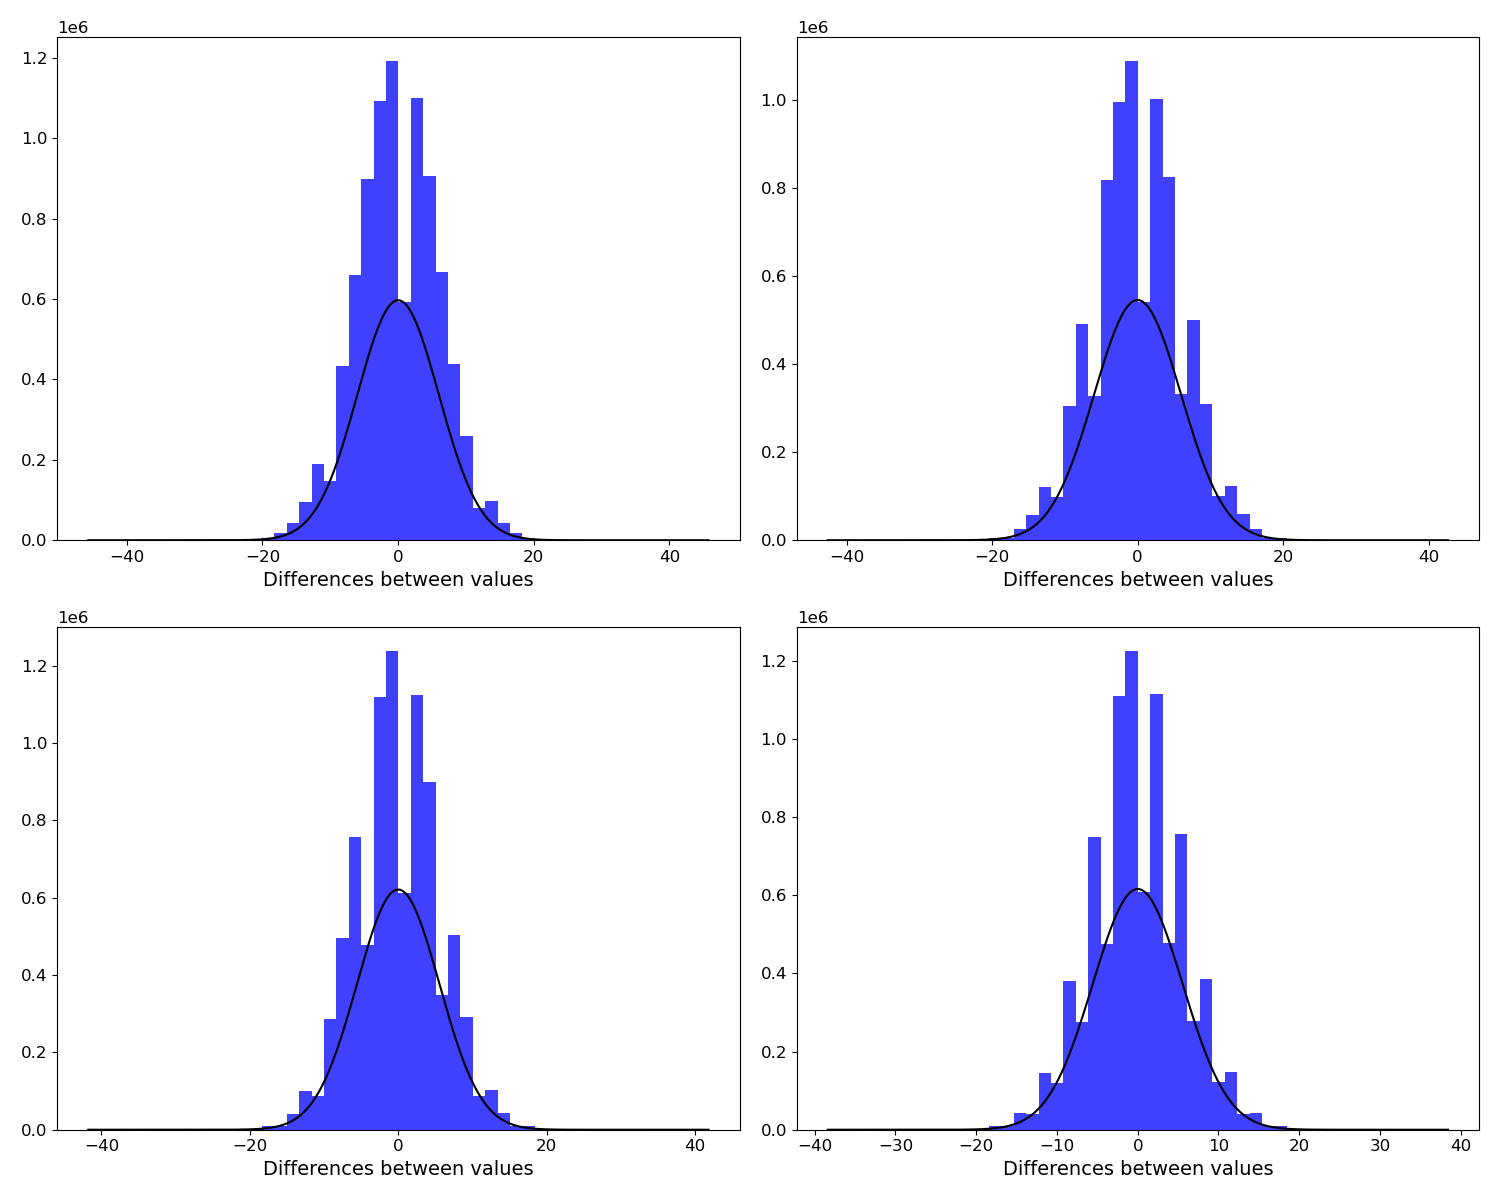
\includegraphics[scale=0.4]{images/biasdiffs.png}
\end{center}   
\caption{This image was constructed by taking all the daily bias files of 17
October 2018, 5 for each of the 4 visible light filters, and noting the
difference between the counts for each pixel between each file and each other
file. A Gaussian fitted to the same mean and standard deviation is overlaid.
In the histograms the very small number of outlying points above 6 standard
deviations is included in the outlying bins. The date was chosen at random, no
other date gave particularly different results.} \protect\label{fig:biasdiffs}
\end{figure}

\subsubsection{Construction of master bias files}
\protect\label{section:mastbiasconstr}

It was of possible concern that the method for constructing the master bias
files set out in Section \ref{section:masterbiasfiles} may include noisy bias
files but whose means are nevertheless within the selected range. By looking at
Fig. \ref{fig:mastmeanbias} a number of places were noted where the plot appears
to wander sharply. In \ref{fig:ibiasnolim} is illustrated the daily bias files
over a period where the master bias files differ quite sharply from month to
month. It is notable that there are some daily bias files with high noise but
also where the mean is close to the overall mean and thus would be included in
the construction of the master bias file. The number of daily bias files over
parts of these periods appears to be limited, with gaps of nearly 2 weeks in
some cases. The corresponding master bias files would appear to be less
reliable in these cases.

By excluding daily bias files with standard deviations less than 3 times the
standard deviation of standard deviations, the spread of daily bias files over
the same period takes the form seen in Fig. \ref{fig:bias3std} is seen. Again
days when no bias files are made as apparent.

\begin{figure}[!htbp]
\begin{center}
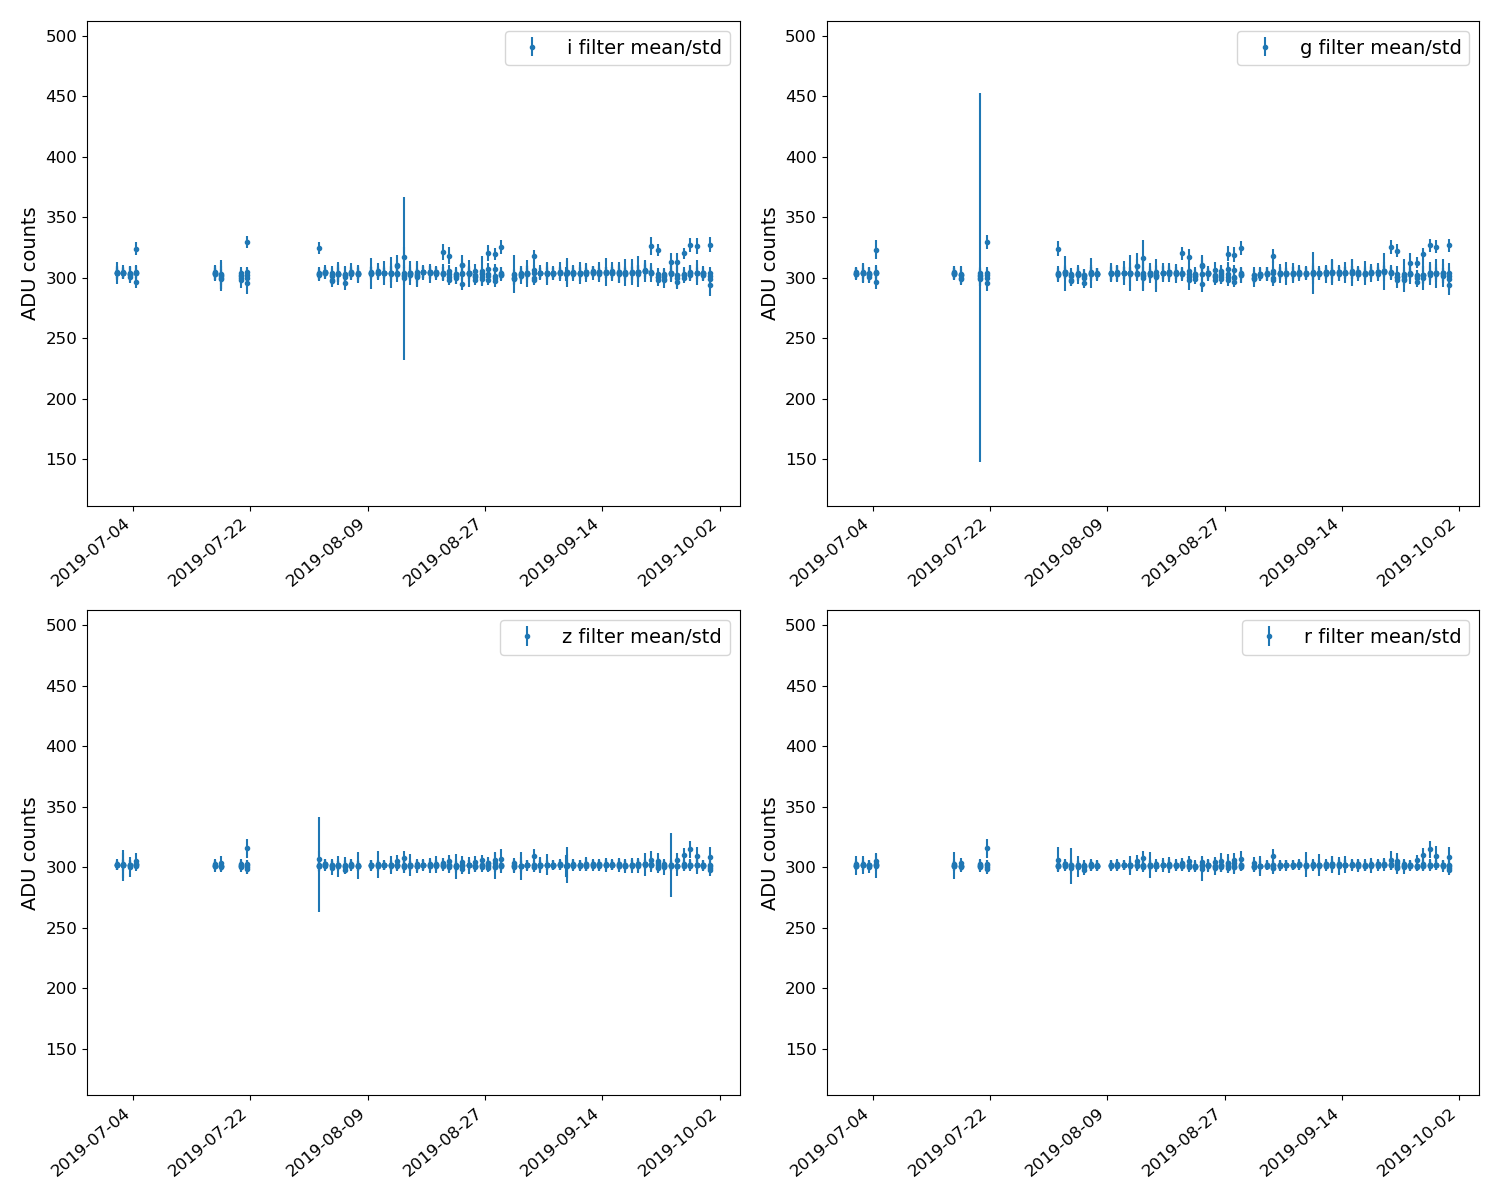
\includegraphics[scale=0.4]{images/ibiasnolim.png}
\end{center}   
\caption{This figure displays the daily bias files over the period July to
September 2019 inclusive showing the means and standard deviations for each
file. This corresponds to a section of Fig. \ref{fig:mastmeanbias} where
the variability is greater.} \protect\label{fig:ibiasnolim}
\end{figure}

\begin{figure}[!htbp]
\begin{center}
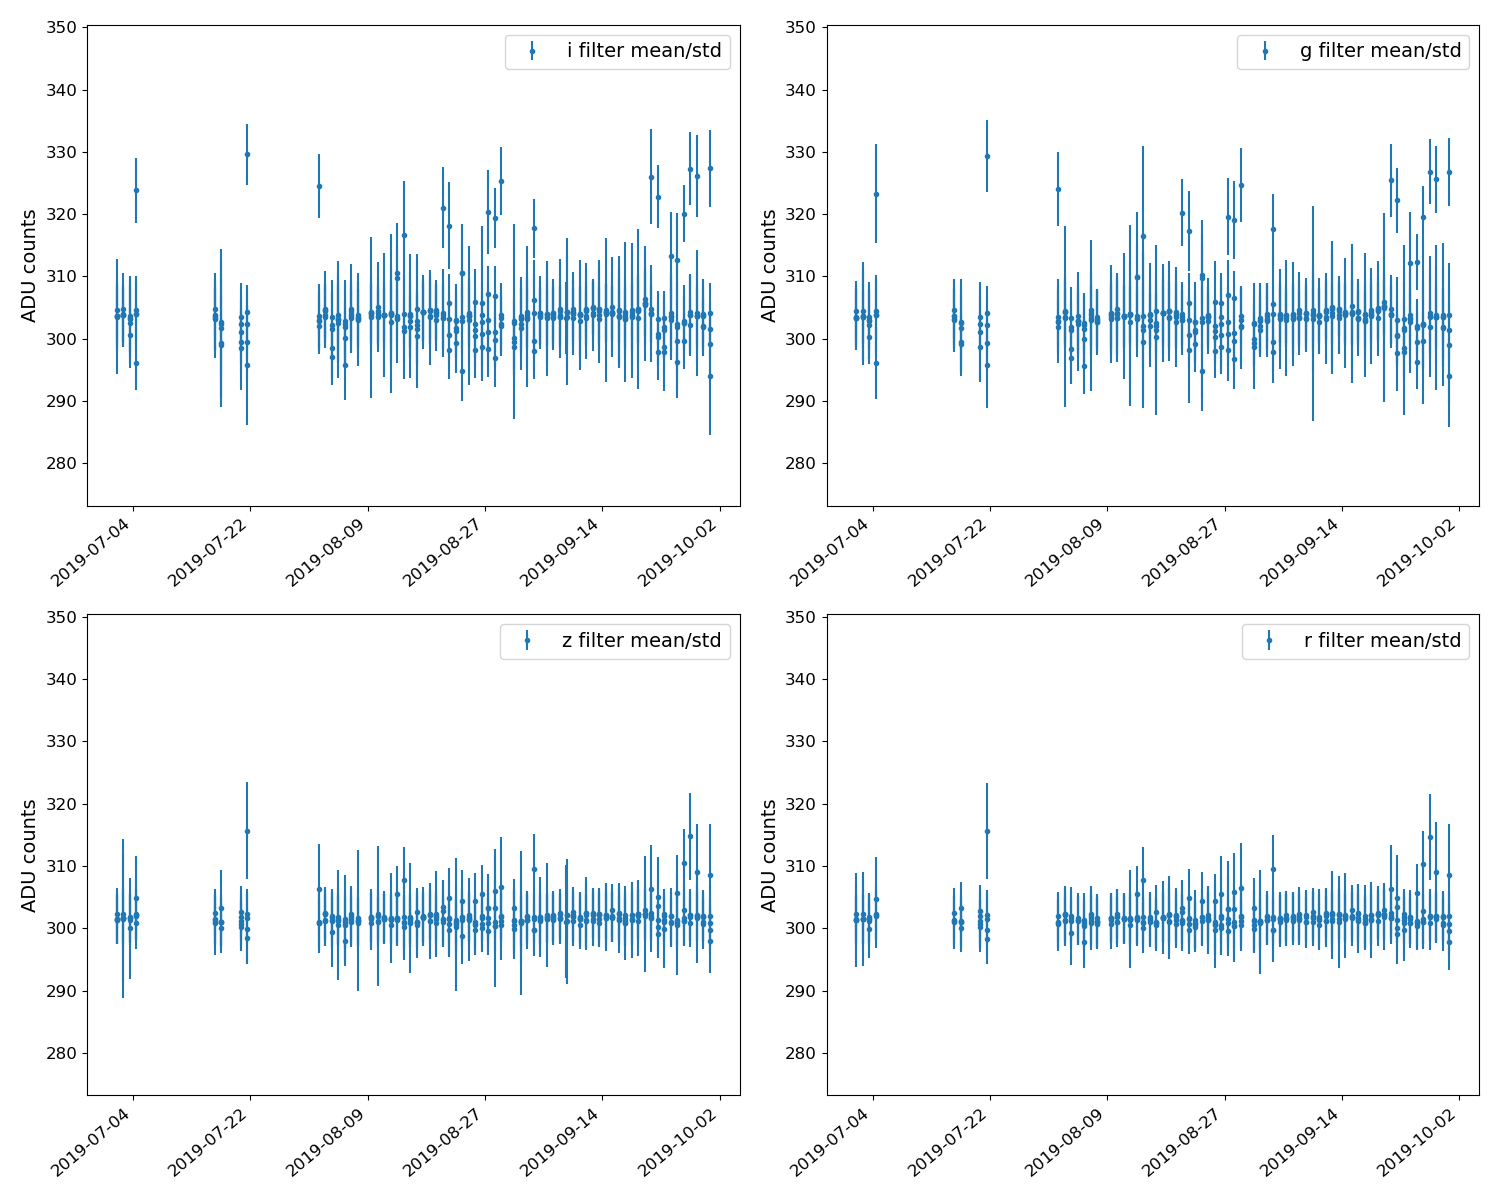
\includegraphics[scale=0.4]{images/ibiaslim3std.png}
\end{center}   
\caption{This figure shows the same daily bias files over the period July
to September 2019 as Fig. \ref{fig:ibiasnolim} but excluding the files whose
standard deviations from the means are greater than 3 times the standard
deviation of standard deviation of the overall standard deviations. Note that
the Y axis has a considerably narrower scale than in Fig. \ref{fig:ibiasnolim}.}
\protect\label{fig:bias3std}
\end{figure}

It would appear from this analysis that the master bias files constructed from
those over the month are not likely to be reliable as they are based upon too
few daily bias files and some of the files included in the construction of the
master bias files are particularly noisy. \textit{I'm going to put in a short study showing
progression of bias levels and noise over time here.}

The conclusion from this study is to replace the master bias files with a
``rolling'' master bias files constructed from a window of bias files with, as
far as possible, the same number of daily bias files either side. It should be
noted that the processing of the most recent observational images will have to
be redone later to take into account later daily bias files giving a window
symmetric about the observation dates. This is not expected to make a
large difference, but for completeness, it is done.

As the noise on each pixel varies considerably, rather than having an overall
value for the standard deviation of the constructed master bias file, it costs
little in terms of additional resources to calculate and use a separate standard
deviation value for each pixel.

\clearpage

\subsection{Analysis of flat files}
\protect\label{section:flatanal}

The images displayed in the previous sections utilised the master flat files for
the appropriate month (in addition to the master bias files). First these files
were considered, before turning to the daily flat files, from which these are
constructed.

\subsubsection{Master flat files}
\protect\label{section:mastflats}

The image in Fig. \ref{fig:initgexample} and the images in Fig.
\ref{fig:init4example} were processed using the master flat and bias files for
September 2018. In Fig. \ref{fig:mastfeg0918} is illustrated the master flat
file for each filter. (The master bias file for each filter is shown in Fig.
\ref{fig:mastbeg0918} and discussed in Section \ref{section:biasanal}.) For
comparison, the master flat file for January 2020 is shown in Fig.
\ref{fig:mastfeg0120}. (The master bias file for January 2020 is shown in Fig.
\ref{fig:mastbeg0120} in Section \ref{section:biasanal}.) The reason for
including this latter image is that the telescope configuration was changed
slightly in March 2019.

\begin{figure}[!htbp]
\begin{center}
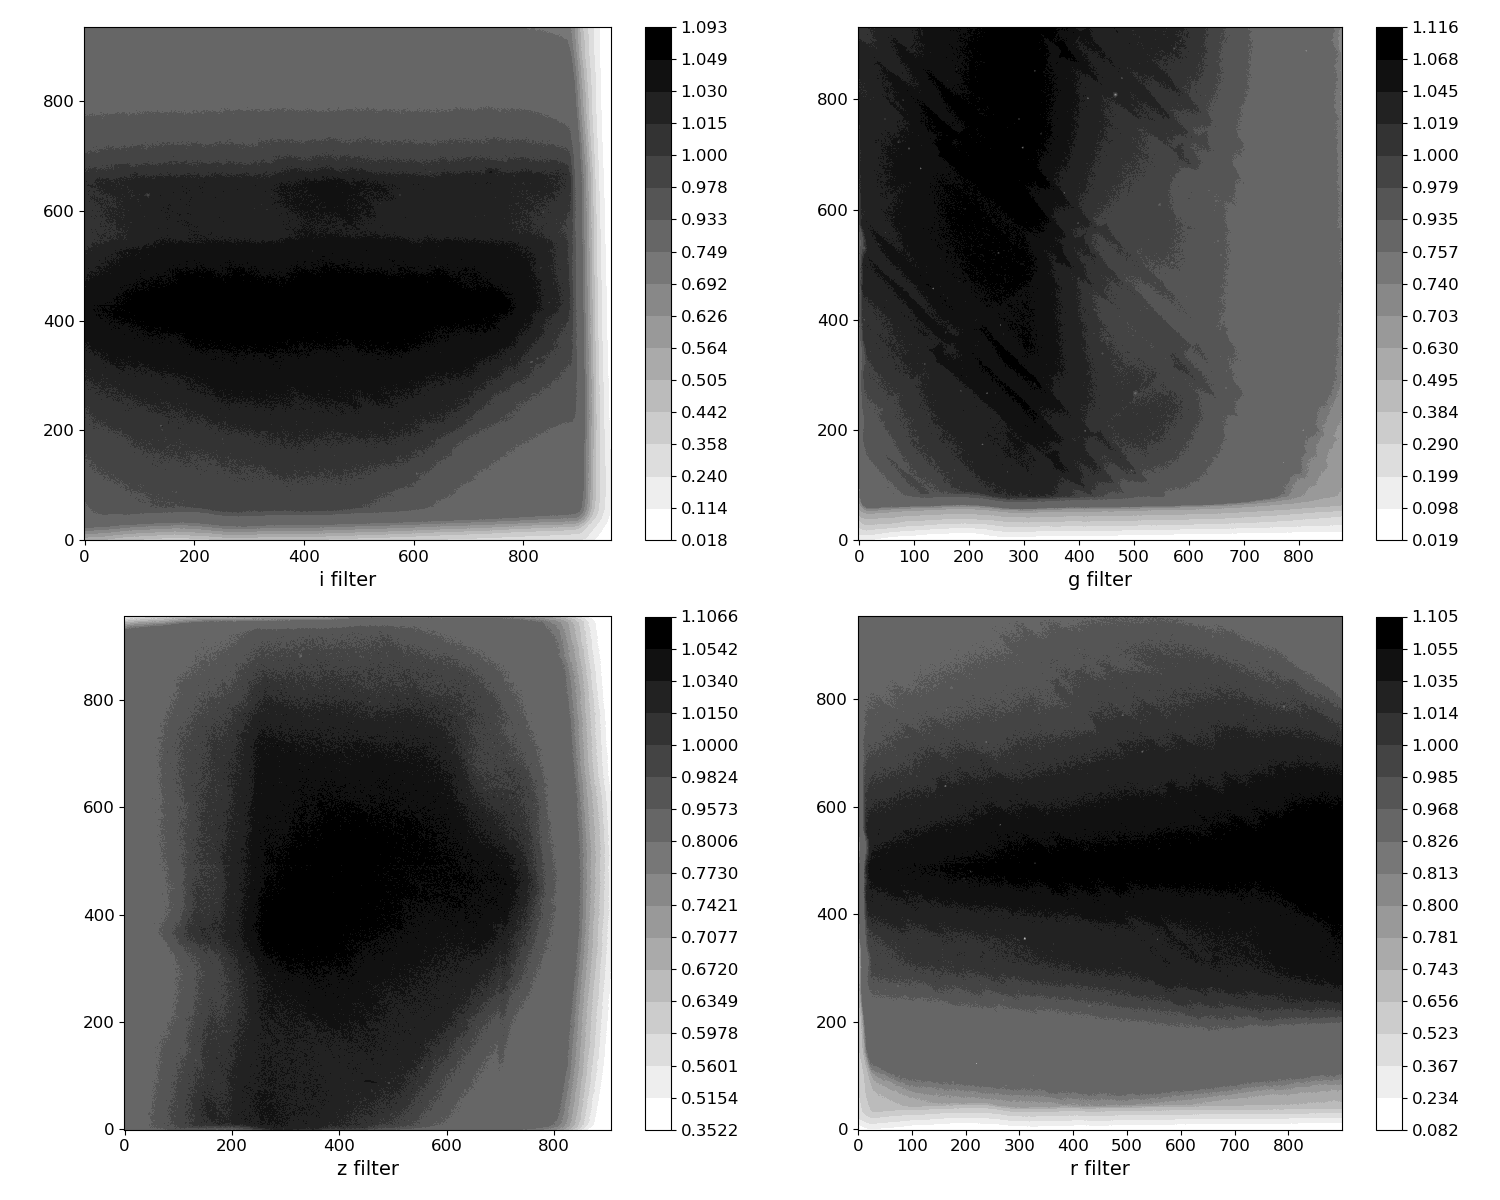
\includegraphics[scale=0.4]{images/mastflateg0918.png}
\end{center}   
\caption{This illustrates the 4 master flat files for each filter used to
construct Fig. \ref{fig:initgexample} and Fig. \ref{fig:init4example}. The
positions of the 4 images reflect the positions and orientations in which the
images are taken from the CCD.}
\protect\label{fig:mastfeg0918}
\end{figure}

\begin{figure}[!htbp]
\begin{center}
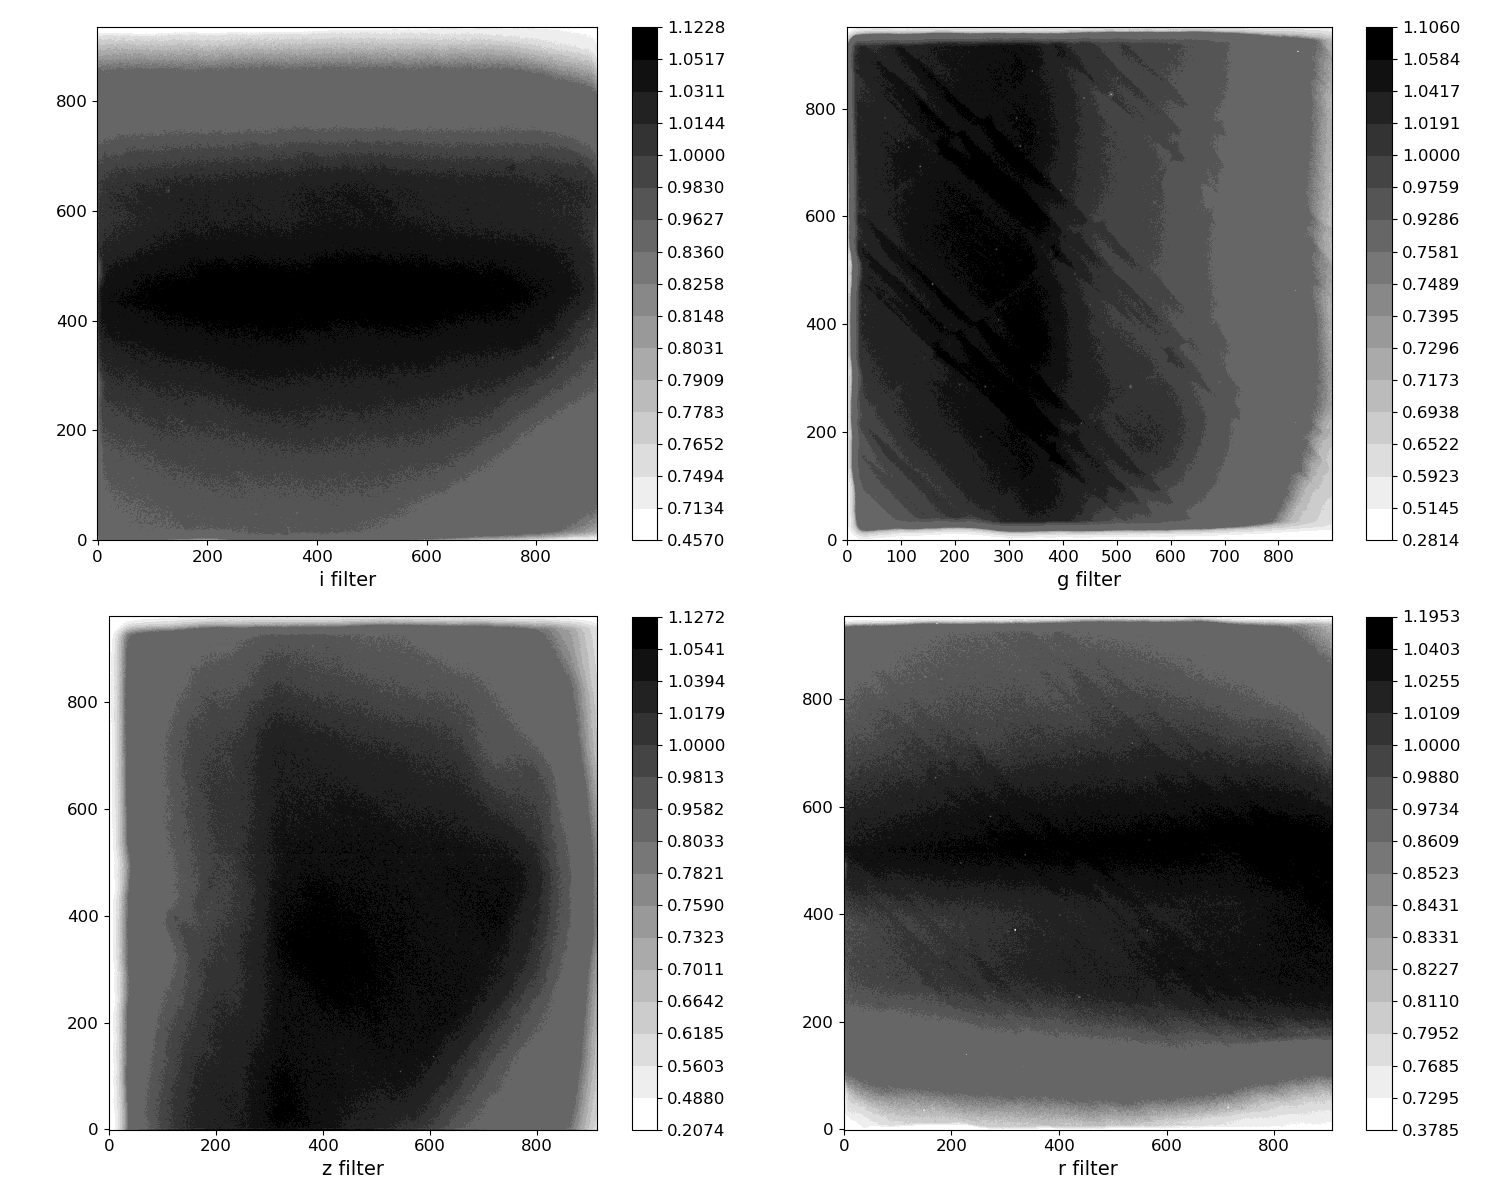
\includegraphics[scale=0.4]{images/mastflateg0120.png}
\end{center}   
\caption{This illustrates the 4 master flat files for each filter for January
2020, for comparison with Fig. \ref{fig:mastfeg0918}. The differences are due
to changes in the area and starting positions on the CCD for images made in
March 2019.} \protect\label{fig:mastfeg0120}
\end{figure}

It will be noticed that some of the edges of the master flat fields show low
counts per pixel (the values are normalised). In particular the bottom edges of
the \texttt{g} and \texttt{r} filters and the right edges of the \texttt{i} and
\texttt{z} filters are thus affected. In Fig. \ref{fig:complats1820} is shown a
side by side comparison of the master flats used to prepare Fig.
\ref{fig:initgexample} and Fig. \ref{fig:initgexample20}. Note that the master
bias has already been subtracted from the master flats, so the pixels in the
master flat files are used to divide into the corresponding pixels in the
observation images (following subtraction of the bias file). Hence a low value
in the flat file will yield a higher value in the image to which the flat field
has been applied.

\begin{figure}[!htbp]
\begin{center}
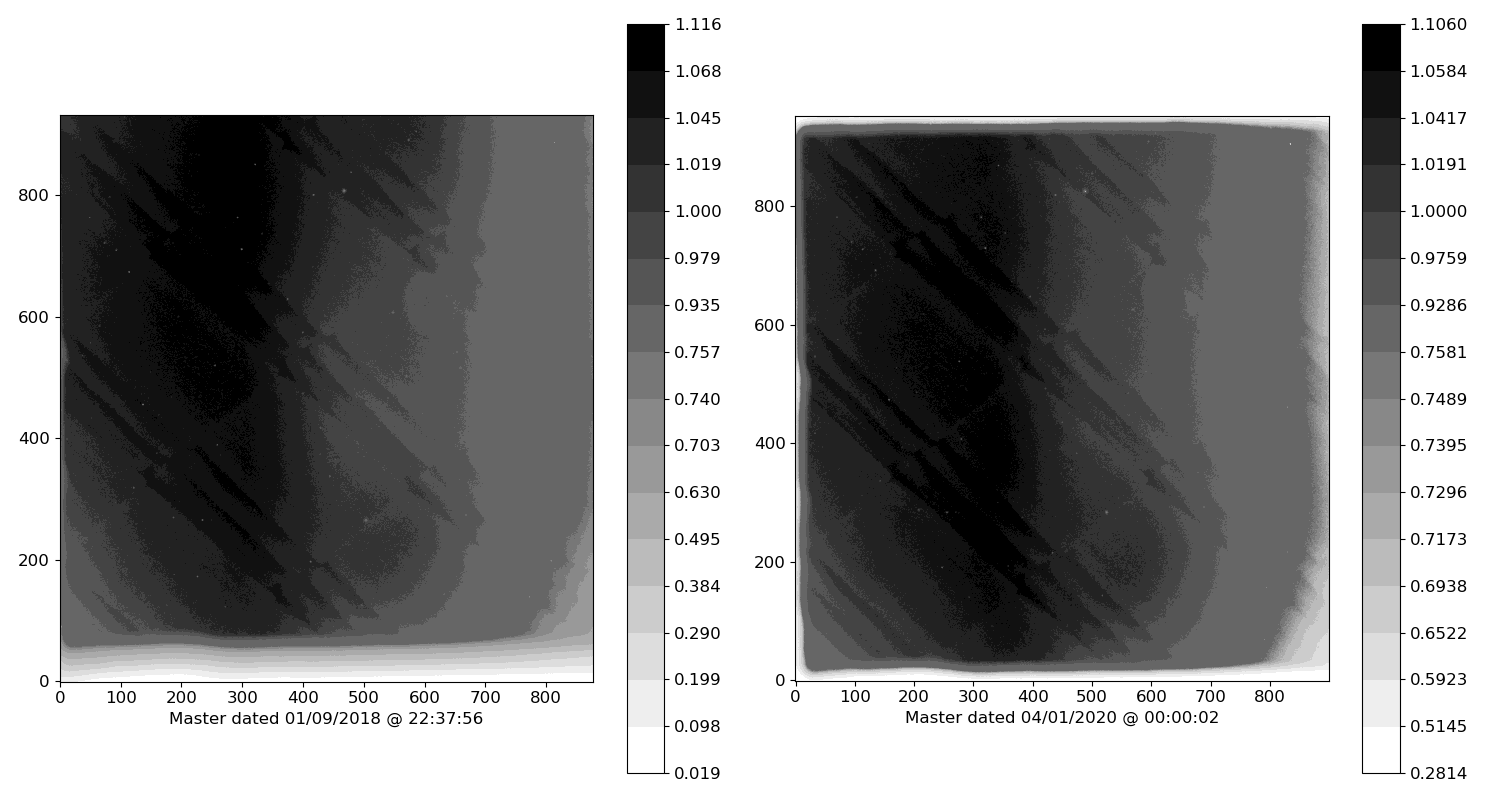
\includegraphics[scale=0.4]{images/complats1820.png}
\end{center}   
\caption{This shows side-by-side the master flat files used to display Fig.
\ref{fig:initgexample} and Fig. \ref{fig:initgexample20}.}
\protect\label{fig:complats1820}
\end{figure}

It might be supposed that this is a problem of the particular pixels concerned.
but if reference is made back to Fig. \ref{fig:showusedccd} earlier it can be
seen that the later observations are taken from a wider area of the CCD than the
earlier ones. For convenience, in Fig. \ref{fig:gfiltareas1820} is shown the
section from Fig. \ref{fig:showusedccd} relating to the \texttt{g} filter and
showing the regions of the CCD used. It can be seen that the area used for the
later observations is larger, especially where the shading is observed at the
bottom of the images. The conclusion reached, and other filters show a
similar story, is that this is more likely to be an issue of the
construction of the telescope, such as vignetting and the like, than problems
with the CCD as the images are set out as projected onto the CCD in these diagrams (there is no rotation of any
image which can be deduced by inspection of sets of observations such as in
Fig. \ref{fig:initgexample} which appear broadly the same). Division by the low
values in these areas will significantly reduce the contrast in the processed
images.

\begin{figure}[!htbp]
\begin{center}
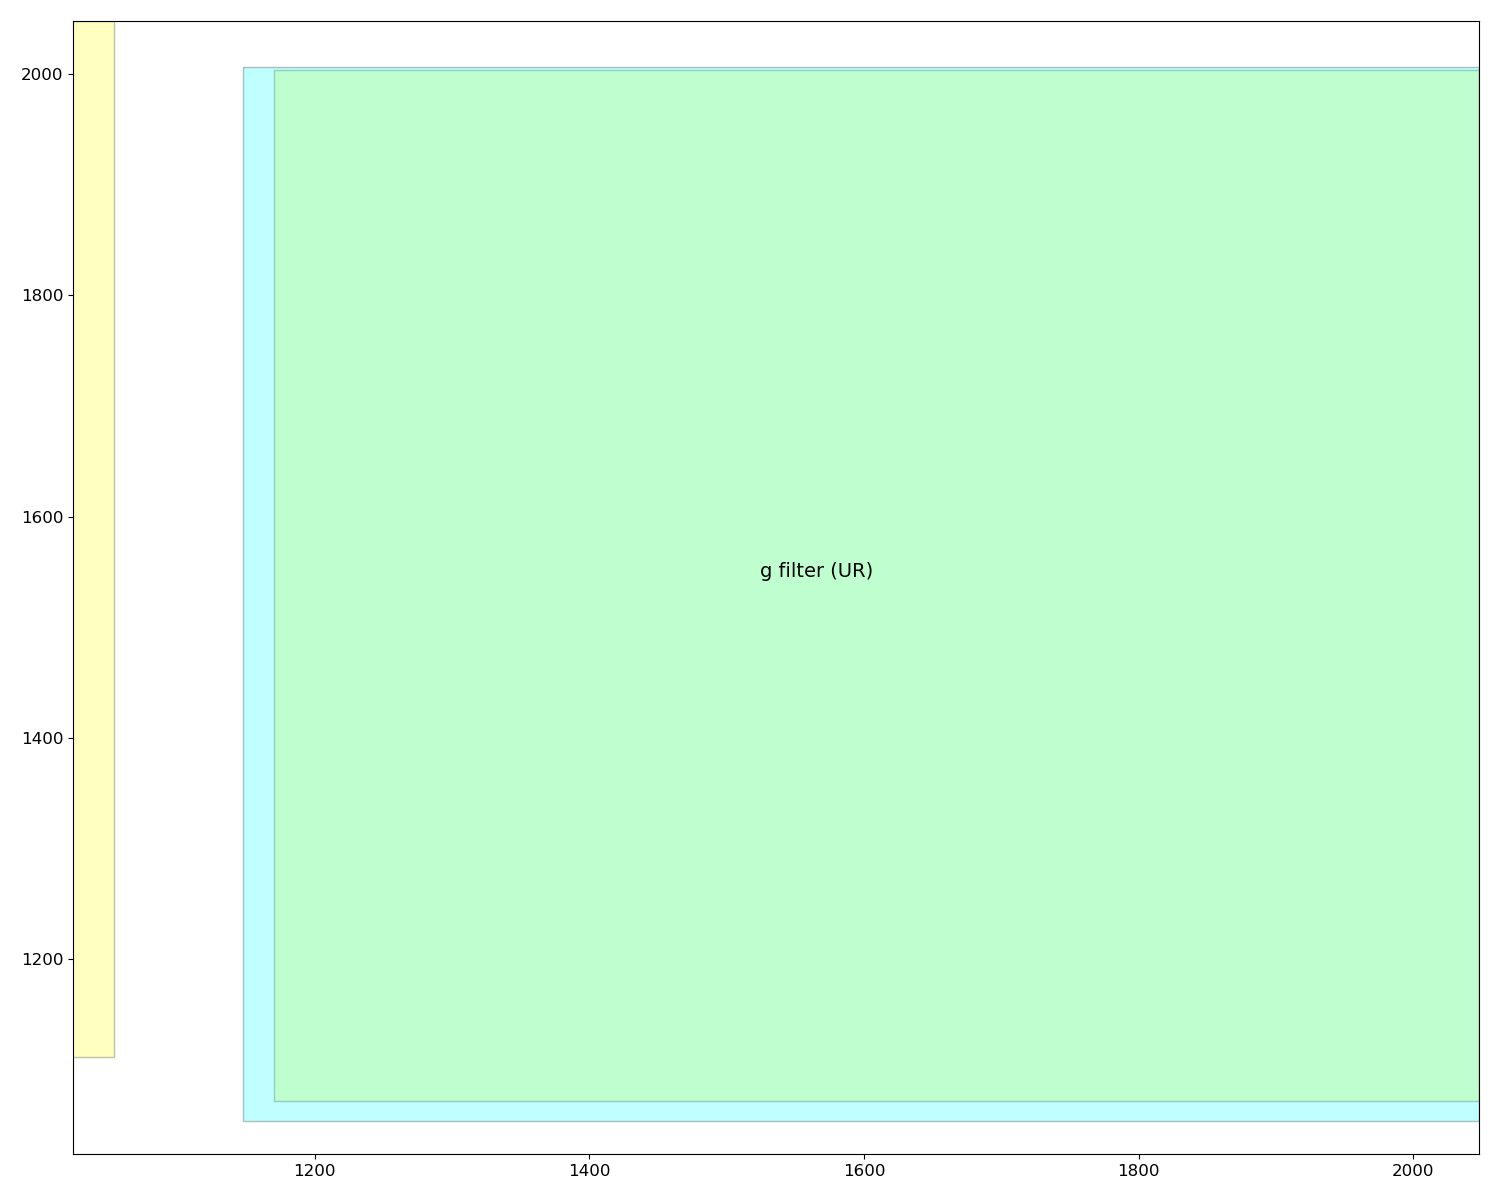
\includegraphics[scale=0.2]{images/gfiltareas1820.png}
\end{center}   
\caption{This is a portion of Fig. \ref{fig:showusedccd} indicating the areas
of the CCD used for the \texttt{g} filter in 2018 and 2020. The cyan region
shows the area used in 2020 and the yellow the area used in 2018. The common
area appears as green. It can be seen that the larger area is that used in 2020
which suggests tat the lower signal seen at the bottom of the image in 2018}
\protect\label{fig:gfiltareas1820}
\end{figure}

As described in \citet{molinari14}, the visible light into the ROSS2 camera is
divided by one dichroic filter into the \texttt{g} and \texttt{r} part and
the \texttt{i} and \texttt{z} parts. Each of those are divided by a further
dichroic filter into the \texttt{g} and \texttt{r} and the \texttt{i} and
\texttt{z} components respectively. Possibly this could be associated with
vignetting or similar brought about by mounting of the dichroic filters. It is
to be noticed that in Fig. \ref{fig:mastfeg0120}, following minor reconfiguration,
this is reduced somewhat.

The master flat files are very similar in content until the reconfiguration in
March 2019. In Fig. \ref{fig:mastmean} is illustrated the mean and standard
deviation of the pixel values in the master flat files over the period of
observation of the {\rdwarf} objects.

\begin{figure}[!htbp]
\begin{center}
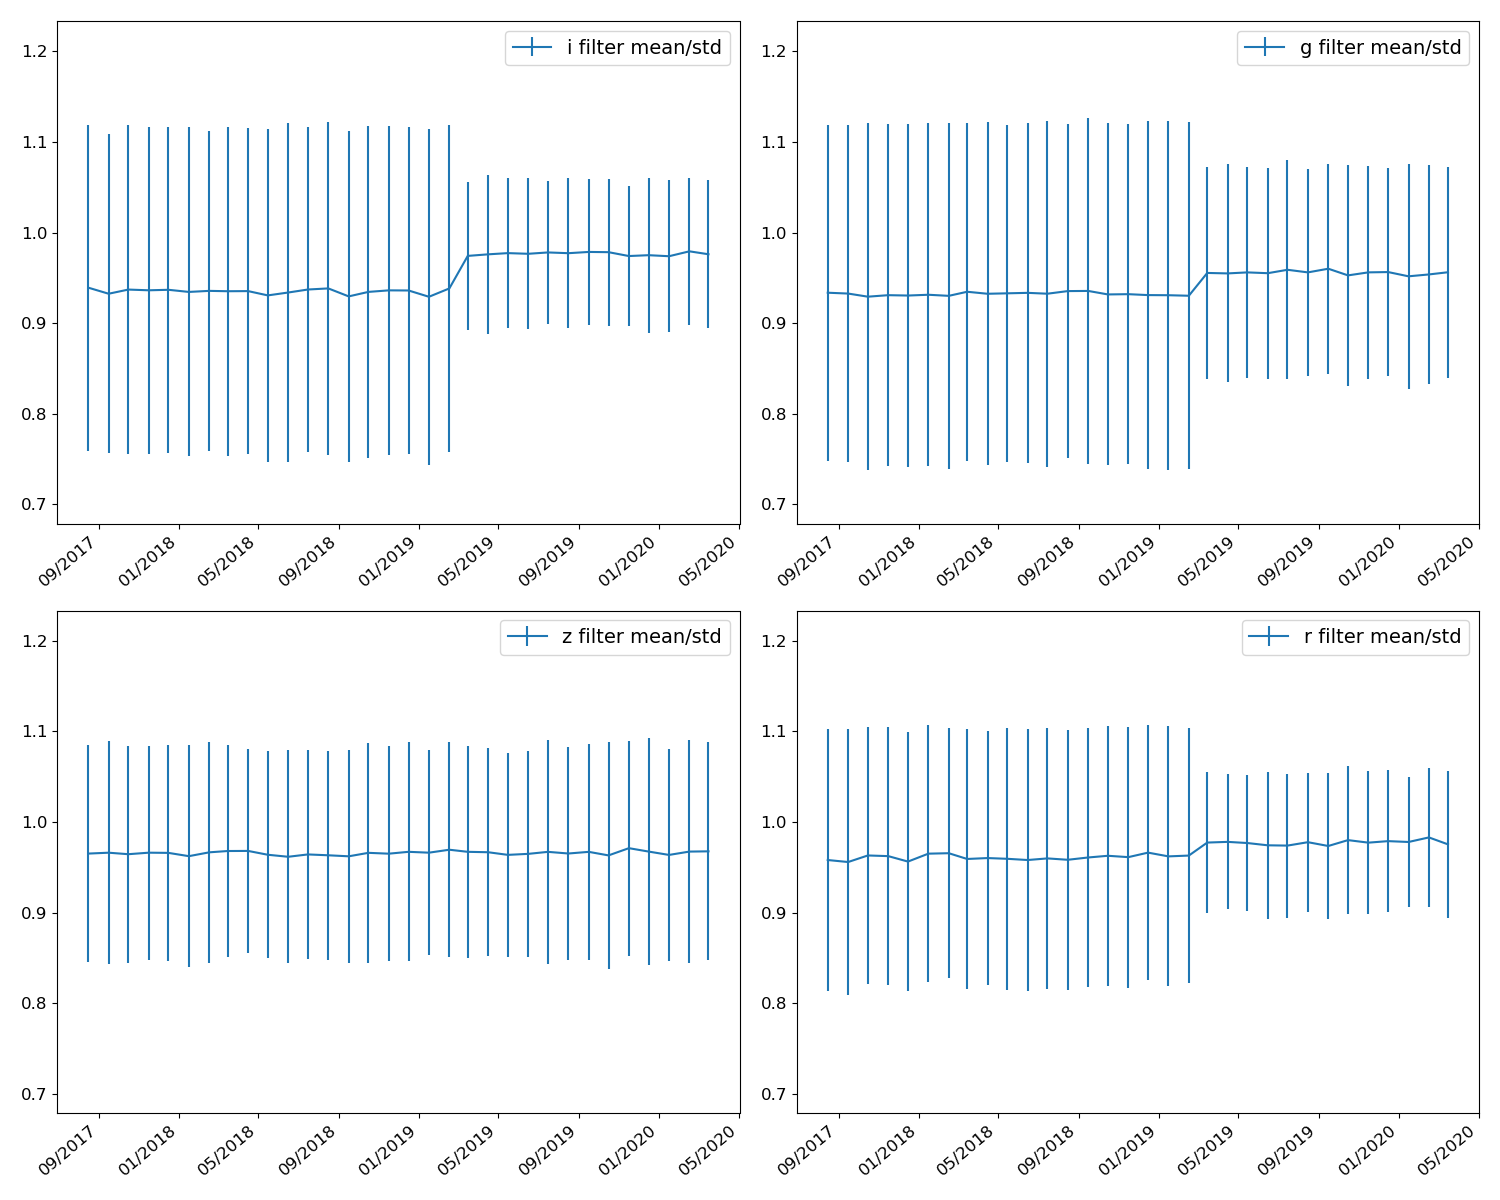
\includegraphics[scale=0.4]{images/mastmean.png}
\end{center}   
\caption{This illustrates the mean and the standard deviation of the values in
the master flat files from July 2017, when {\rdwarf} targets were first
observed, until March 2020. Note the step in March 2019, following
reconfiguration of the telescope.}
\protect\label{fig:mastmean}
\end{figure}

The reconfiguration of the telescope in March 2019 clearly improved the
performance at the edges of the images. It would appear that it would be
desirable to trim the edges of the images, or at the very least give reduced
weighting to photometry taken from these edges.

\subsubsection{Construction of master flat files}
\protect\label{section:constructmff}

Examination of the IDL code used to construct the master flat files revealed
that the master flat files were constructed using the daily flat files for the
relevant month, selected according to the criteria.

\begin{enumerate}
  \item The mean values of the pixel counts falls within the range 5,000 and
  50,000.
  \item The skewness of the distribution of the pixel counts is negative.
  \item The kurtosis of the distribution of the pixel counts is less than 7.
\end{enumerate}

All of these criteria are applied; a daily flat file is not selected if it does
not meet all these criteria. The justification for using the skewness and
kurtosis in this way is not clear.

Regrettably the calculation of the mean, skewness and kurtosis is not correct,
due to a programming error. Further, the history of the master flat file shows
all daily flat files considered for inclusion, not the ones actually selected.
\footnote{It did not seem a productive use of time to reproduce the programming error
and work out the ``correct'' set of daily flat files which went to make up the
master flat files.}

Finally the pixel values are combined by taking the median value and then
normalised. This would appear to be a mistake as the daily flat files are
typically in groups of three as the light fades and thus only values from the
set of ``middle'' flat files would be selected.

The files are normalised to the median value not the mean, as may be apparent
from Fig. \ref{fig:mastmean}, which shows the mean values.

\subsubsection{Daily flat files}
\protect\label{section:dailyflats}

In order to rework the master flat files, a study of the linearity of the daily
flat tiles was undertaken, together with an assessment of the points at which
daily flat files should not be considered towards making a master flat file.

\subsubsubsection{Study of linearity}
\protect\label{section:linearity}
It seemed useful to examine the linearity of the daily flat files by plotting
the standard deviations of of the values for all the pixels in each image against the means.
This is shown in Fig. \ref{fig:dailyflatall}. It would be  expected that this
would be linear with the standard deviations increasing with the mean pixel
values. It is clear from this that there is good linearity up to close to
saturation (at 65,536 counts) but it tails off approaching this. The limits of
5,000 and 50,000 for the mean values in selection of the files for the master
flat files would appear to be  reasonable. However this merits further
investigation, as shown in Section  \ref{section:lincutoff}.

Of concern is that there appear to be two distinct lines in the results three of
the filters. However further investigation showed that this was before and after
the reconfiguration of the telescope in March 2019. Accordingly this was
repeated restricting pixels to those in the common area before and after the
reconfiguration (this appears in green in Fig. \ref{fig:showusedccd}) and correctly
aligning the pixels in the result, with the result as shown in Fig. \ref{fig:dailyflatscomm}.

\begin{figure}[!htbp]
\begin{center}
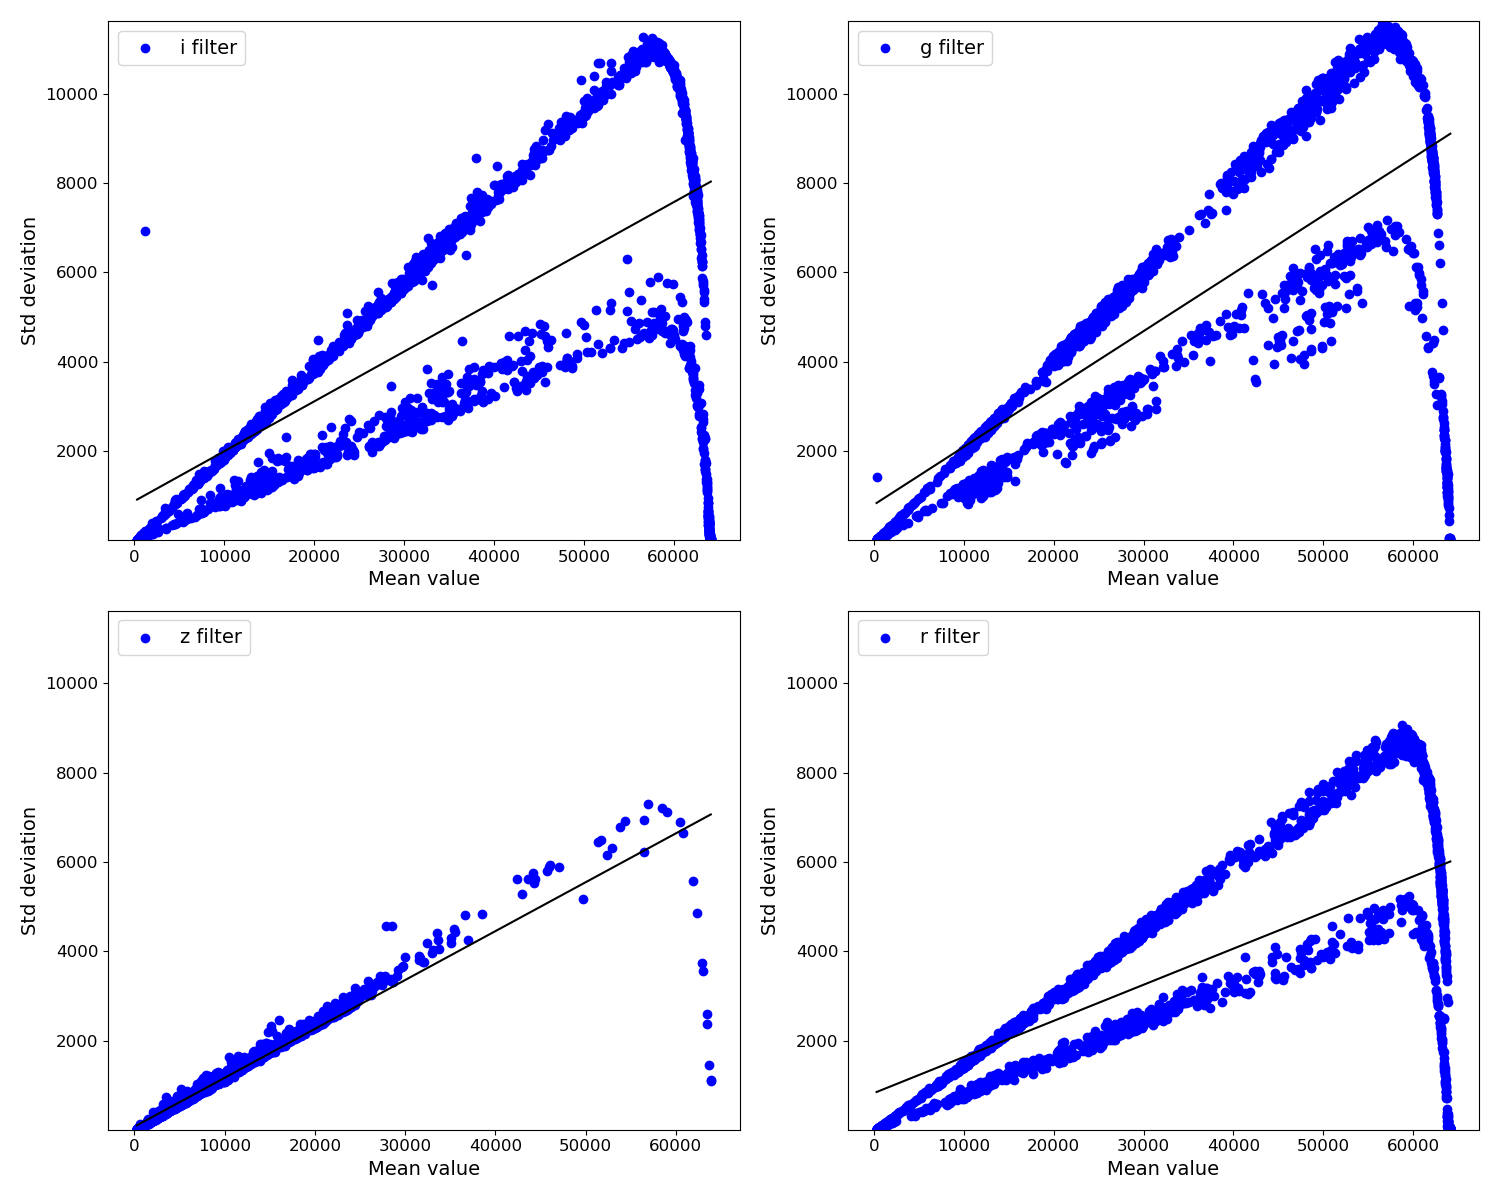
\includegraphics[scale=0.4]{images/dailyflatall.png}
\end{center}   
\caption{This shows the mean plotted against the standard deviations in all
the daily flat files for each of the 4 visible light filters, all to the same
scale. The black line in each case shows the least-squares fit.}
\protect\label{fig:dailyflatall}
\end{figure}

\begin{figure}[!htbp]
\begin{center}
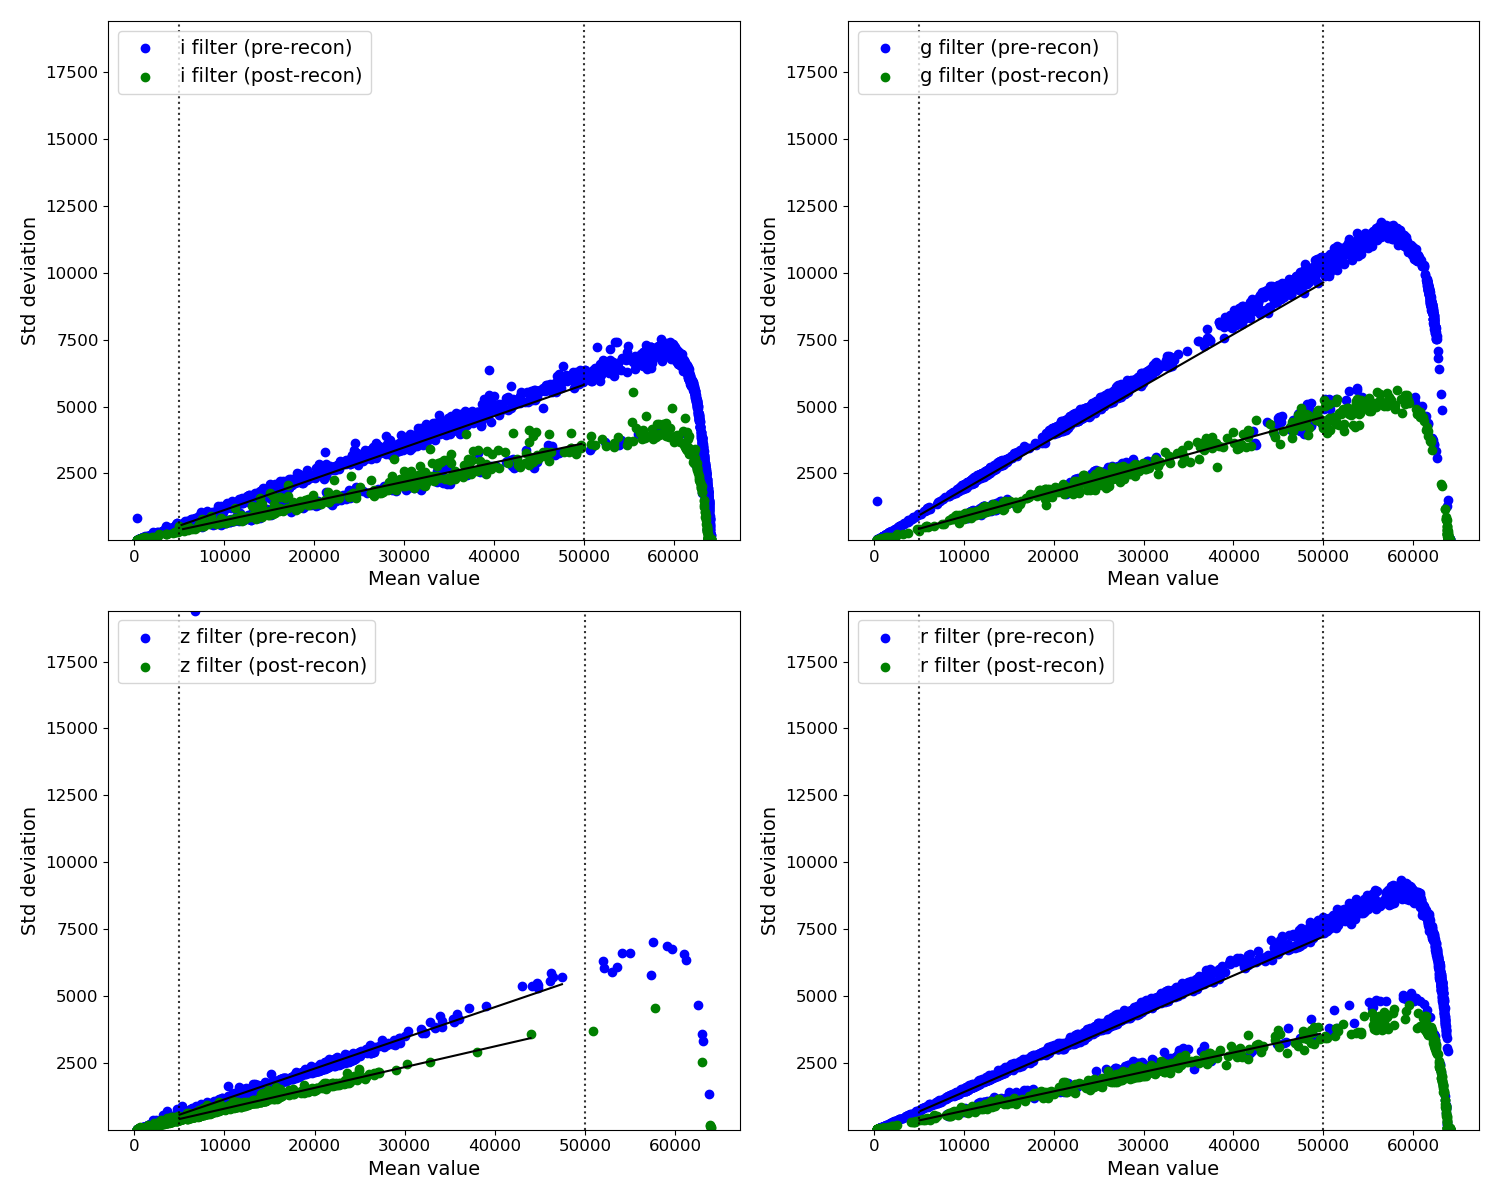
\includegraphics[scale=0.4]{images/dailyflatcomm.png}
\end{center}   
\caption{This figure is equivalent to Fig. \ref{fig:dailyflatall}, but
restricting the pixels to the area of the CCD common to all frames for each
filter and aligning to the same pixels. Points in blue relate to frames taken
prior to March 2019, when the configuration was altered, and those in green
relate to to frames after March 2019. The dotted vertical lines are where the
limits of mean values are taken (at 5,000 to 50,000 counts) in the master flat
files. A least-squares fit was undertaken for frames with mean value within the
limits and this is plotted for each set.}
\protect\label{fig:dailyflatscomm}
\end{figure}

It will be seen from Fig. \ref{fig:mastfeg0918} and Fig. \ref{fig:mastfeg0120}
that the edges tail off, possibly due to vignetting or due to the mounting, do
the plot in Fig. \ref{fig:dailyflatscomm} was repeated for Fig.
\ref{fig:dailyflatstrim}. It will be seen that the linearity agrees much more
substantially. (If the restriction to the common area is not done, this is not
nearly so effective and little difference is made to the display in Fig.
\ref{fig:dailyflatall}.)

\begin{figure}[!htbp]
\begin{center}
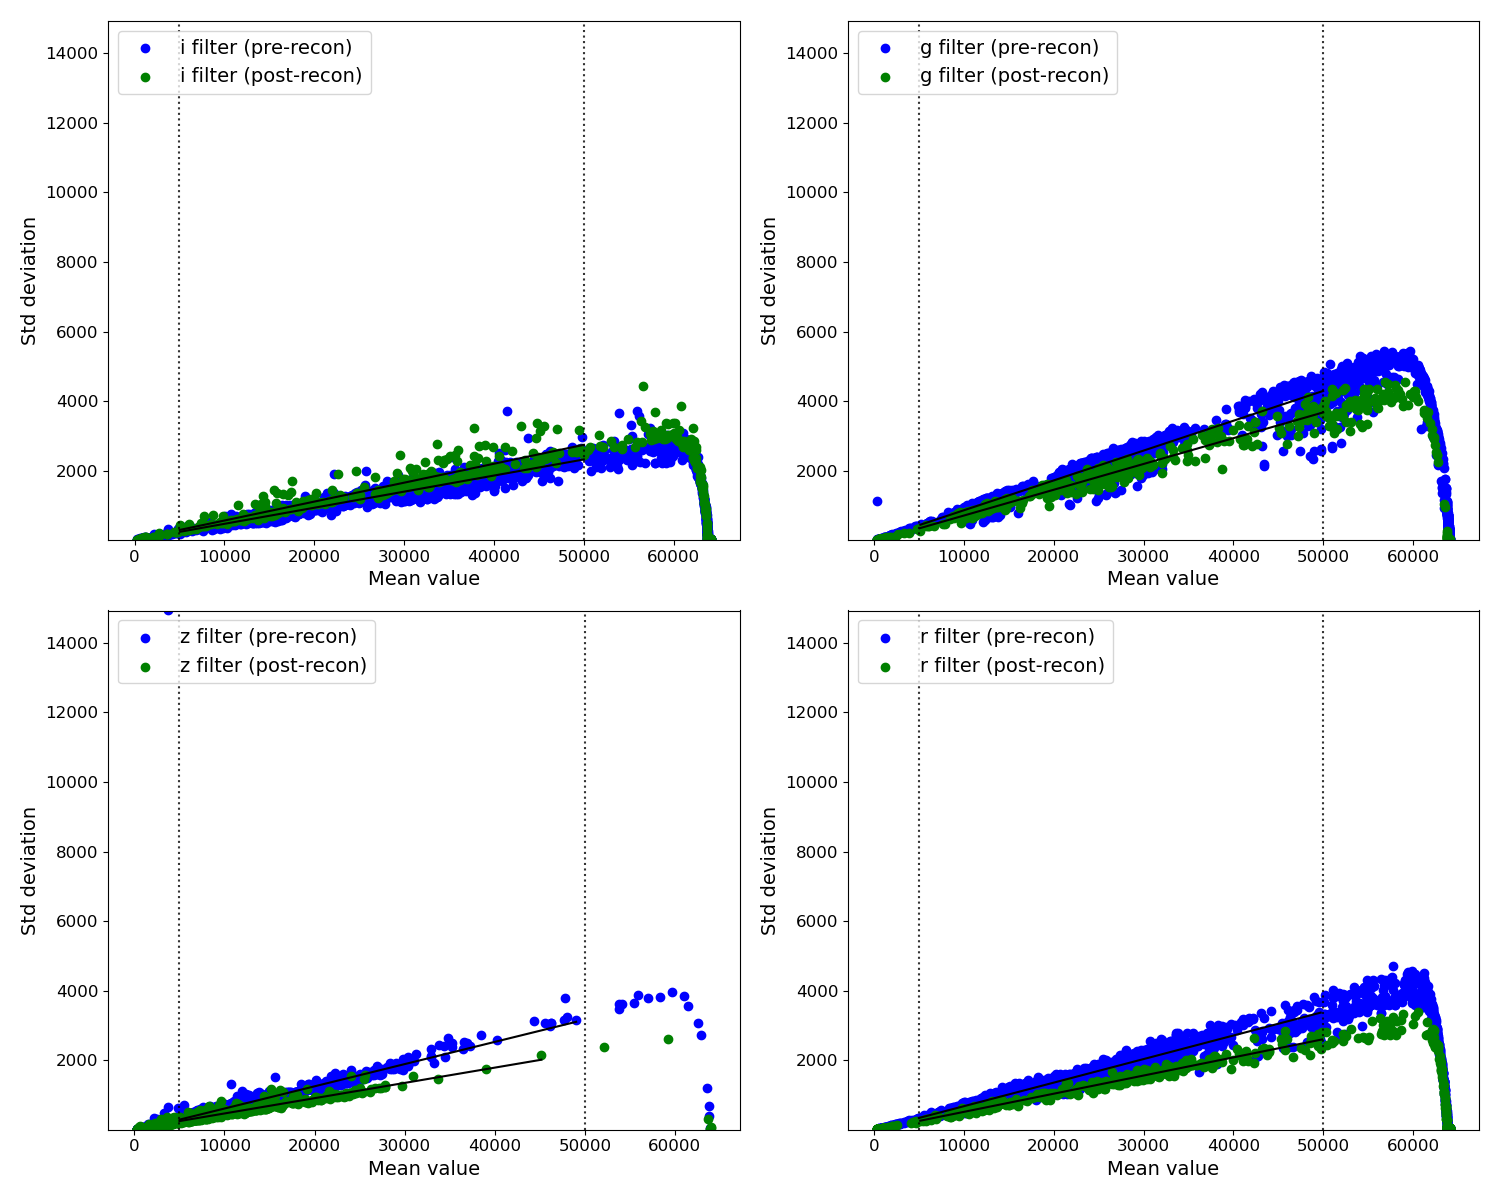
\includegraphics[scale=0.4]{images/dailyflattrim.png}
\end{center}   
\caption{This figure is equivalent to Fig. \ref{fig:dailyflatscomm}, but
additionally 50 pixels are trimmed from each edge of the image.}
\protect\label{fig:dailyflatstrim}
\end{figure}

\subsubsubsection{Linearity cut-offs}
\protect\label{section:lincutoff}

Next examined was the limitation of daily flat files selected for the master
flat to ones with means between 5,000 and 50,000.\footnote{There were other
restrictions, based on the skewness and kurtosis of the distribution, these are
considered further in Section \ref{section:flatselection}.} This was examined by
looking at the correlation coefficients of the fit of the standard deviations to the mean as illustrated in Fig.
\ref{fig:dailyflatscomm} and Fig. \ref{fig:dailyflatstrim}. In Fig.
\ref{fig:lregmaxes} the files are selected with a minimum mean of 10,000 counts
and showing the correlation coefficient of the fig and the standard deviation
with various maximum mean values. In Fig. \ref{fig:lregmins} the daily flat
files are selected with  maximum mean value of 50,000 and various minimum mean
values.

\begin{figure}[!htbp]
\begin{center}
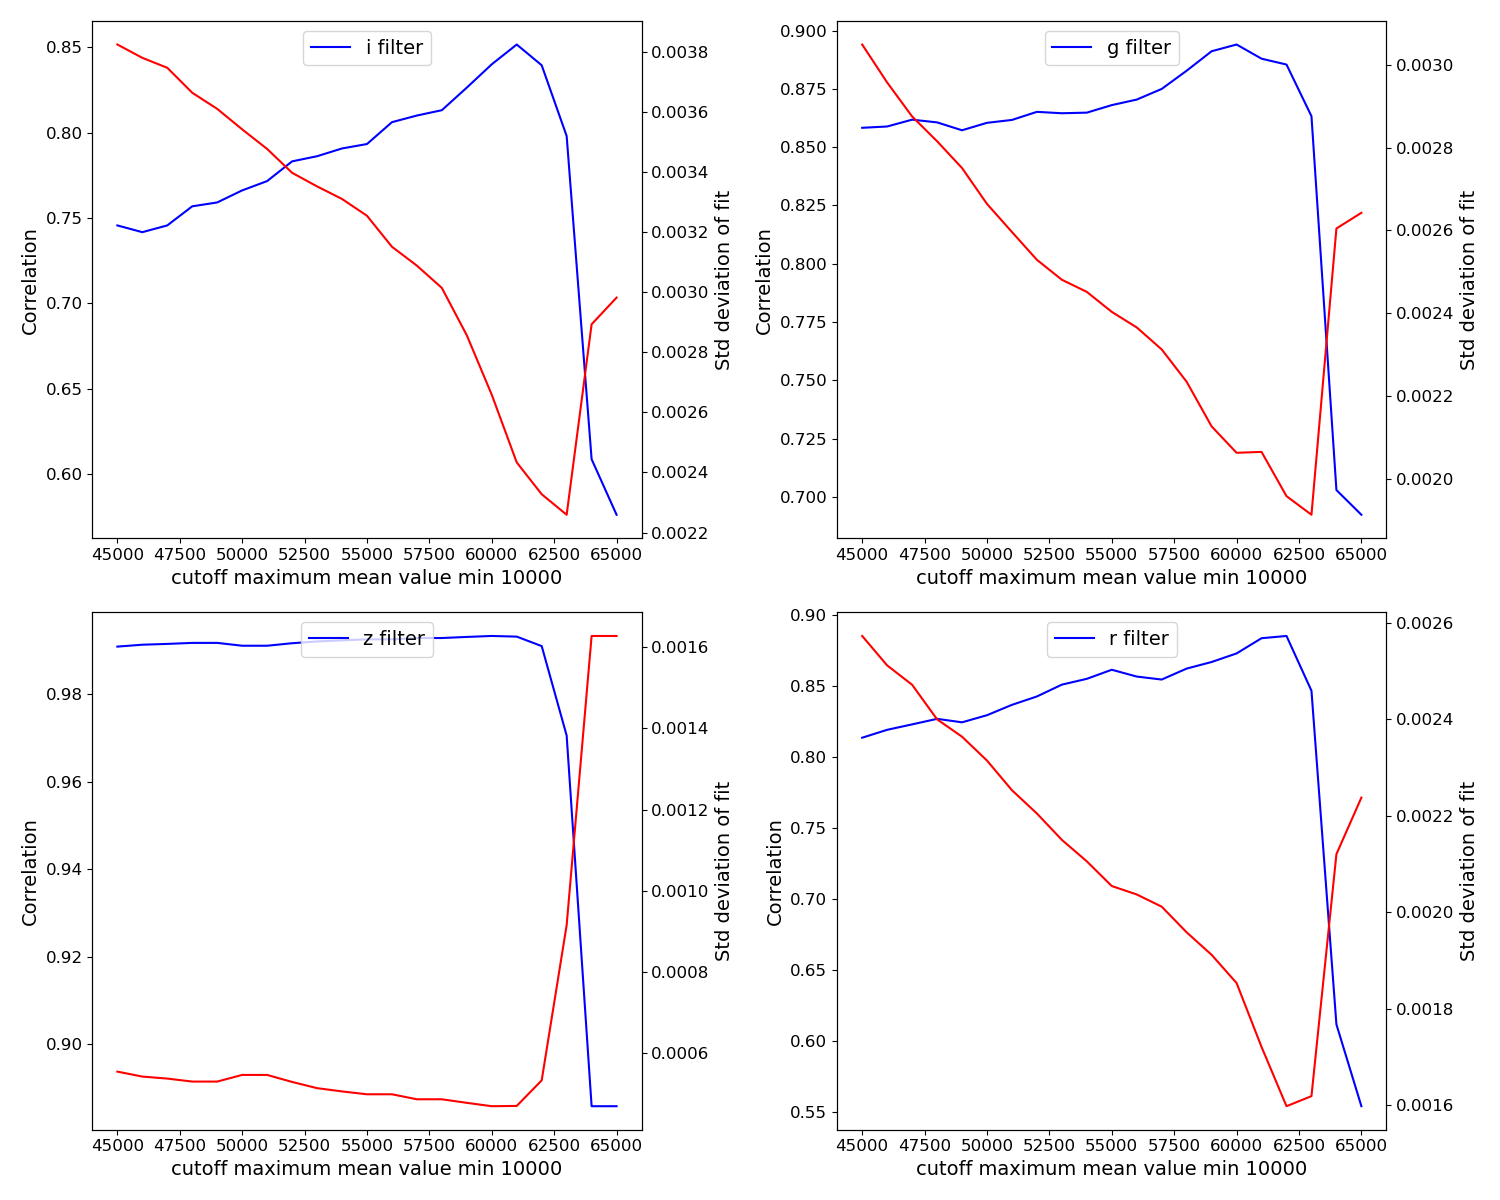
\includegraphics[scale=0.4]{images/lregmaxes.png}
\end{center}   
\caption{This figure was obtained by selecting daily flat files with a minimum
mean value of 10,000 and obtaining the correlation coefficient and standard
deviation of fit with maximum mean value of 45,000 upwards for each filter.}
\protect\label{fig:lregmaxes}
\end{figure}

\begin{figure}[!htbp]
\begin{center}
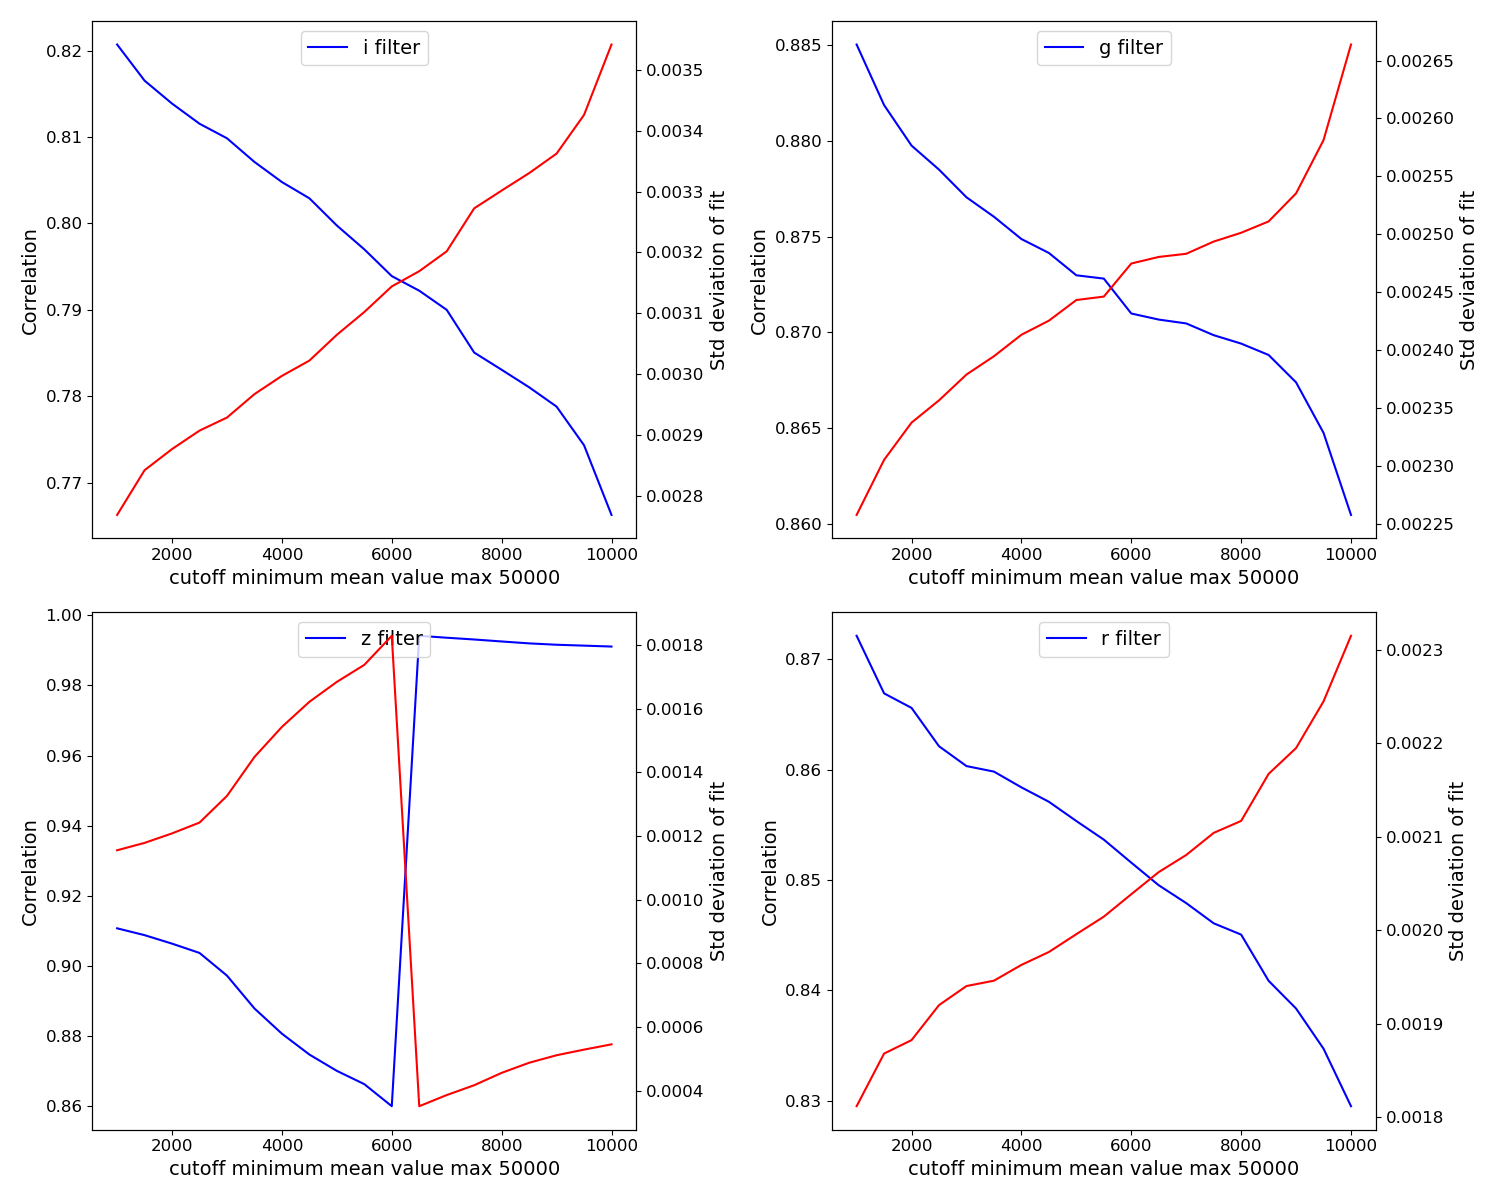
\includegraphics[scale=0.4]{images/lregmins.png}
\end{center}   
\caption{This figure was obtained by selecting daily flat files with a maximum
mean value of 50,000 and obtaining the correlation coefficient and
standard deviation of fit with minimum mean value of 10,000 downwards for each
filter.} \protect\label{fig:lregmins}
\end{figure}

This result might be exactly as expected. As the counts approach the maximum of
65,535, at which the CCD is saturated, the accuracy tails off. At the lower end
of the scale, the signal to noise becomes unacceptably high. It would appear
from these results that a minimum mean of 6,000 would be more appropriate whilst
the maximum mean could safely be raised to 61,000.\footnote{Note that this is
the maximum \underline{mean}, not the maximum \underline{value}, individual
pixels may have a higher value, but frames including the maximum of 65,535 counts should be avoided as
they are likely to be saturated.} Raising the lower level of the mean in this
way would lose the following percentages of daily flat files. It was found that
raising the lower limit of means lost less than 0.5\% of the files, but this was
more than made up for by the increased number of files made eligible for
selection by raising the upper limit to 61,000. This is illustrated in Table
\ref{table:selectedflats}.

The files lost are not seen as particularly significant especially as the files
involved are those with the lowest counts, for which the signal to noise, after
subtraction of the bias files, is inevitably worst. The reverse is true for the
files gained by raising the upper limit.

\subsubsubsection{Selection of daily flat files}
\protect\label{section:flatselection}

With the guidelines taken from the analysis of linearity, it was deemed
appropriate to study the selection of flat files to make up the master flat
files. As stated above in Section \ref{section:constructmff}, this was on the
basis of the means falling within a range of 5,000 to 50,000, together with
further constraints that the skewness of the distribution of pixel values being
negative and the kurtosis being below 7.

In Fig. \ref{fig:flatdispall} are shown the distributions of the means, standard
deviations, skewness and kurtosis for all the daily flat files. If this is
constrained to consider only files with pixel means between 6,000 and 61,000 the
distributions become simpler as shown in Fig. \ref{fig:flatdisplims} and if
files with a standard distribution over 10,000 (representing nearly 20\% of the
maximum pixel value) are omitted, the distributions become as shown in Fig.
\ref{fig:flatdisplimssd10000}.

With reasonable limitations on the flat files, limiting the maximum standard
deviations to 10,000 (it will be clear from \ref{fig:flatdispall} that the
majority are much less than this), that files with positive skewness are reduced
to zero and those with kurtosis over 7 are negligible (under 0.01\%).

It therefore considered that selection based on skewness or kurtosis adds little
benefit\footnote{Even if they were correctly calculated.} and hence for
construction of alternative master flat files, these were omitted.

\begin{figure}[!htbp]
\begin{center}
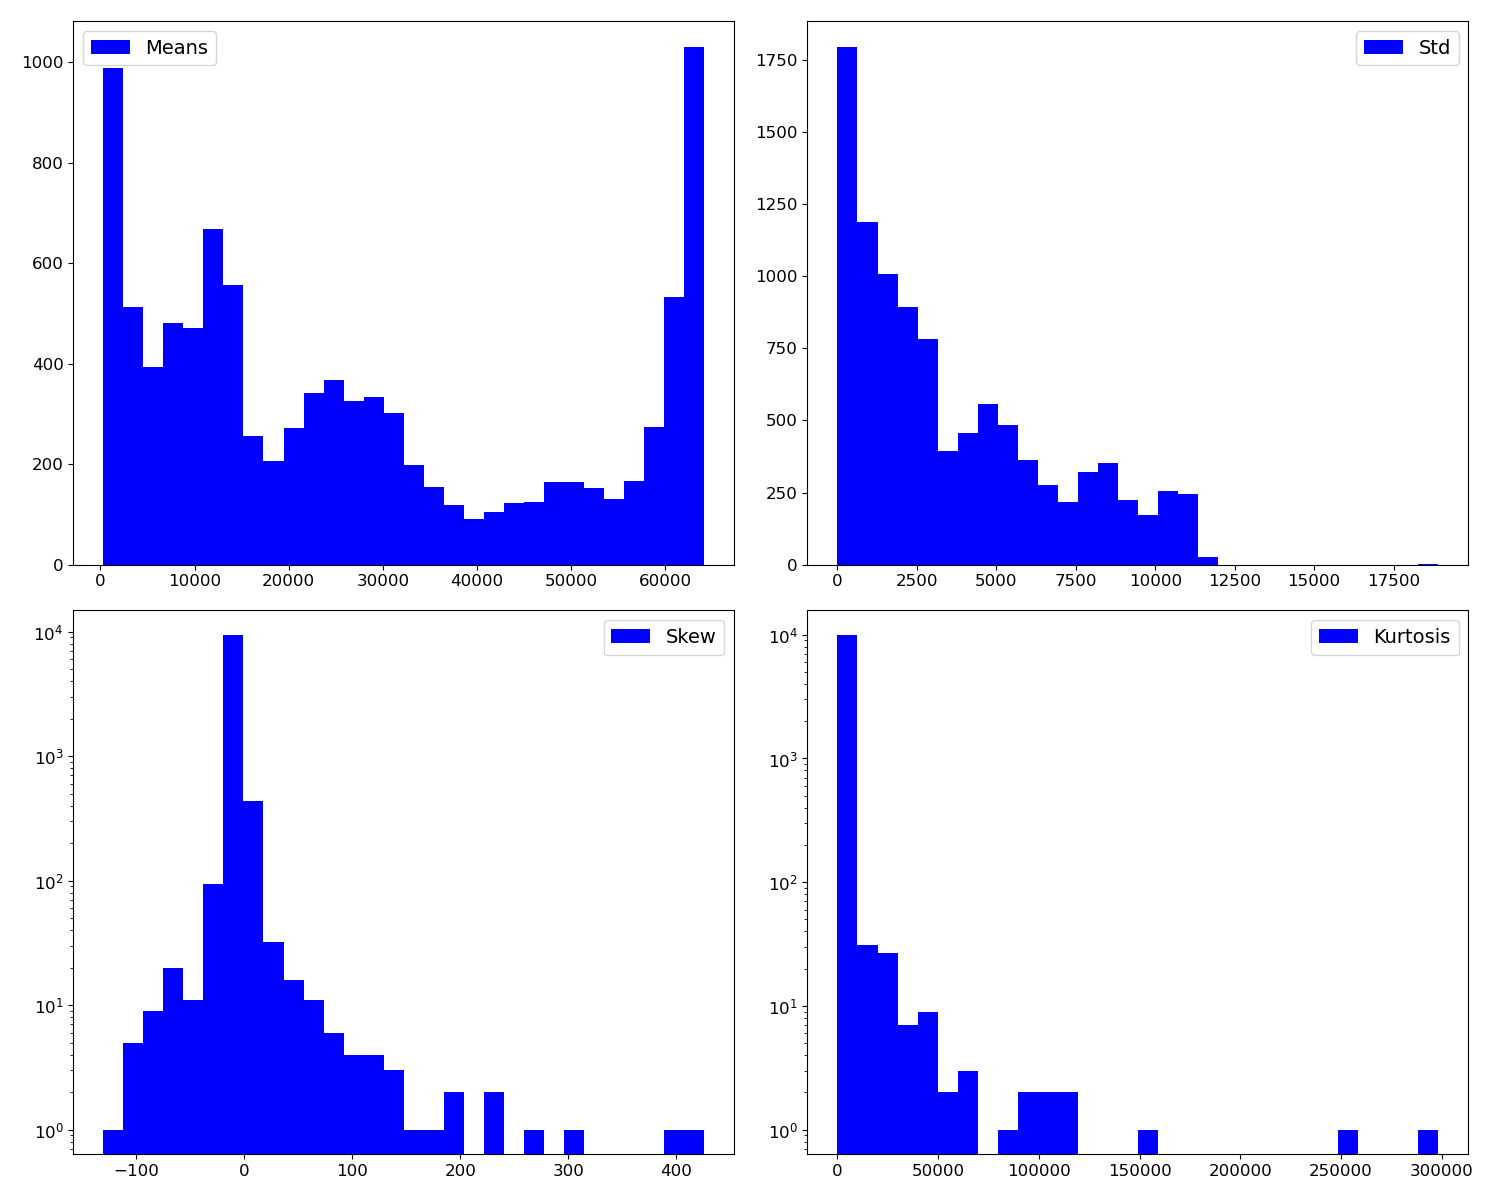
\includegraphics[scale=0.4]{images/flatdispall.png}
\end{center}   
\caption{This figure shows the distribution of means, standard deviations,
skewness and kurtosis of the pixel values of the daily flat files for the
visible light filters. The skewness and kurtosis histogram are displayed on a
logarithmic scale.} \protect\label{fig:flatdispall}
\end{figure}

\begin{figure}[!htbp]
\begin{center}
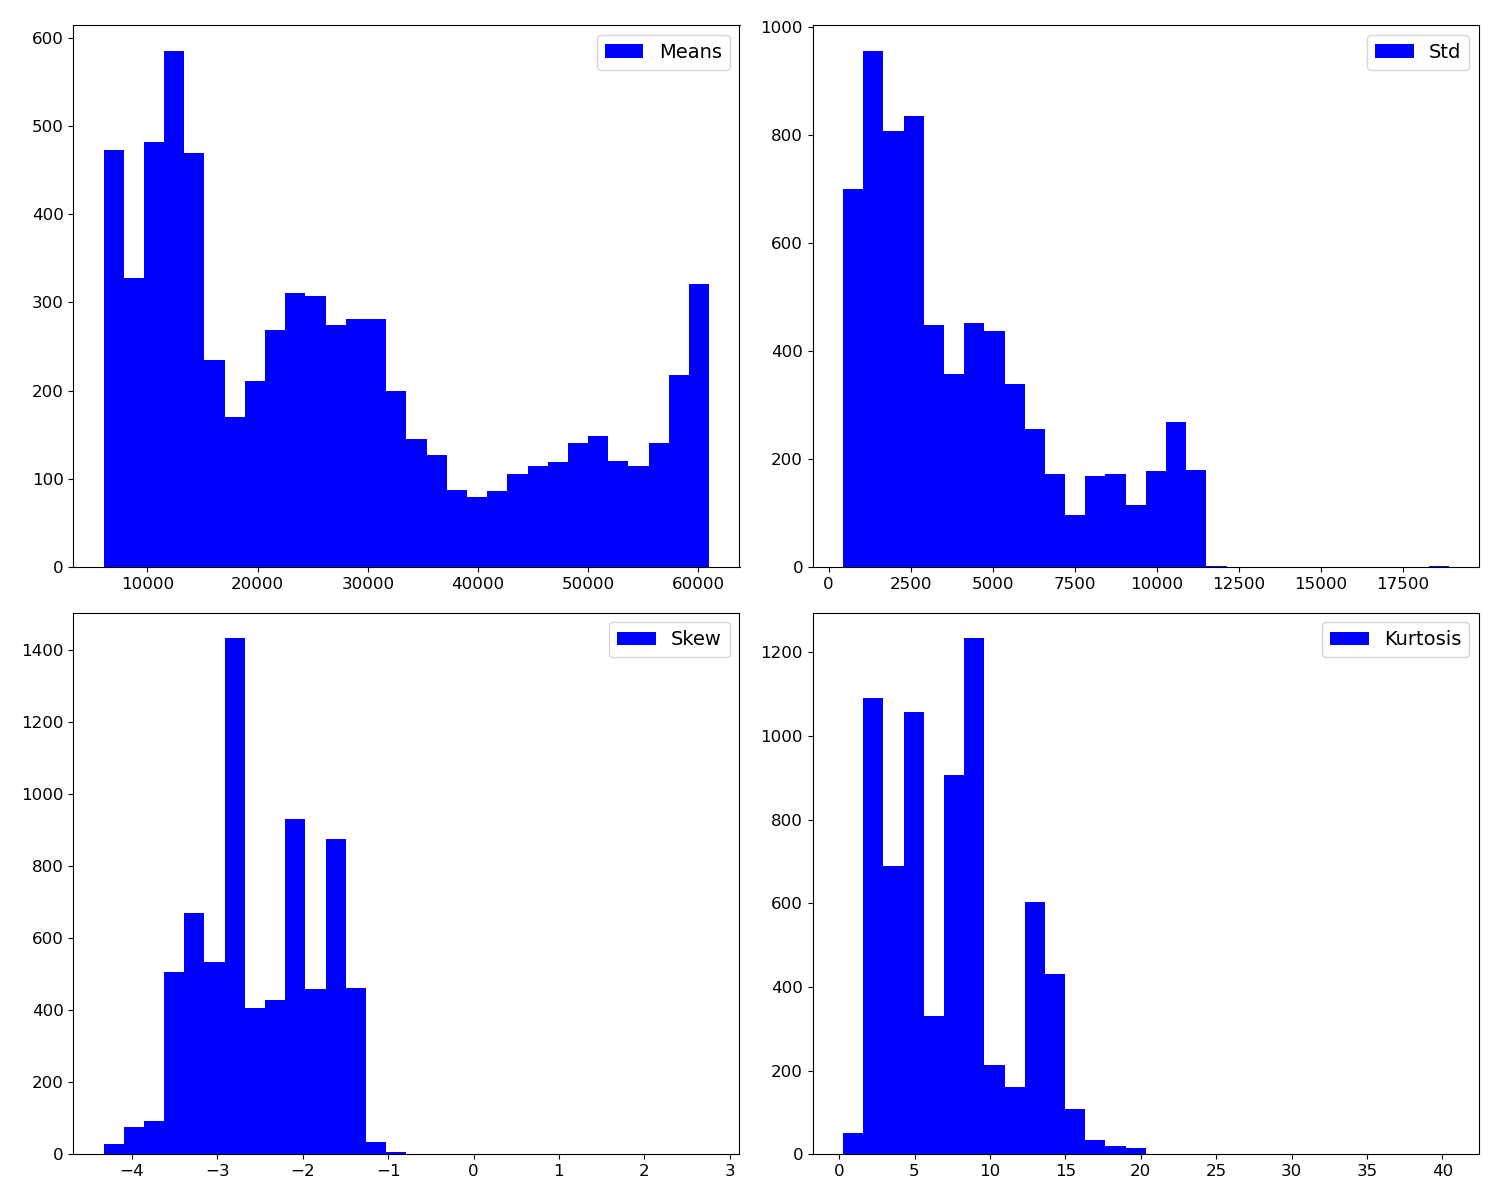
\includegraphics[scale=0.4]{images/flatdisplims.png}
\end{center}   
\caption{This figure is the same data as for Fig. \ref{fig:flatdispall} except
flat files with mean pixel values lower than 6,000 or over 61,000 are
omitted.The skewness and kurtosis are not shown on a logarithmic scale.}
\protect\label{fig:flatdisplims}
\end{figure}

\begin{figure}[!htbp]
\begin{center}
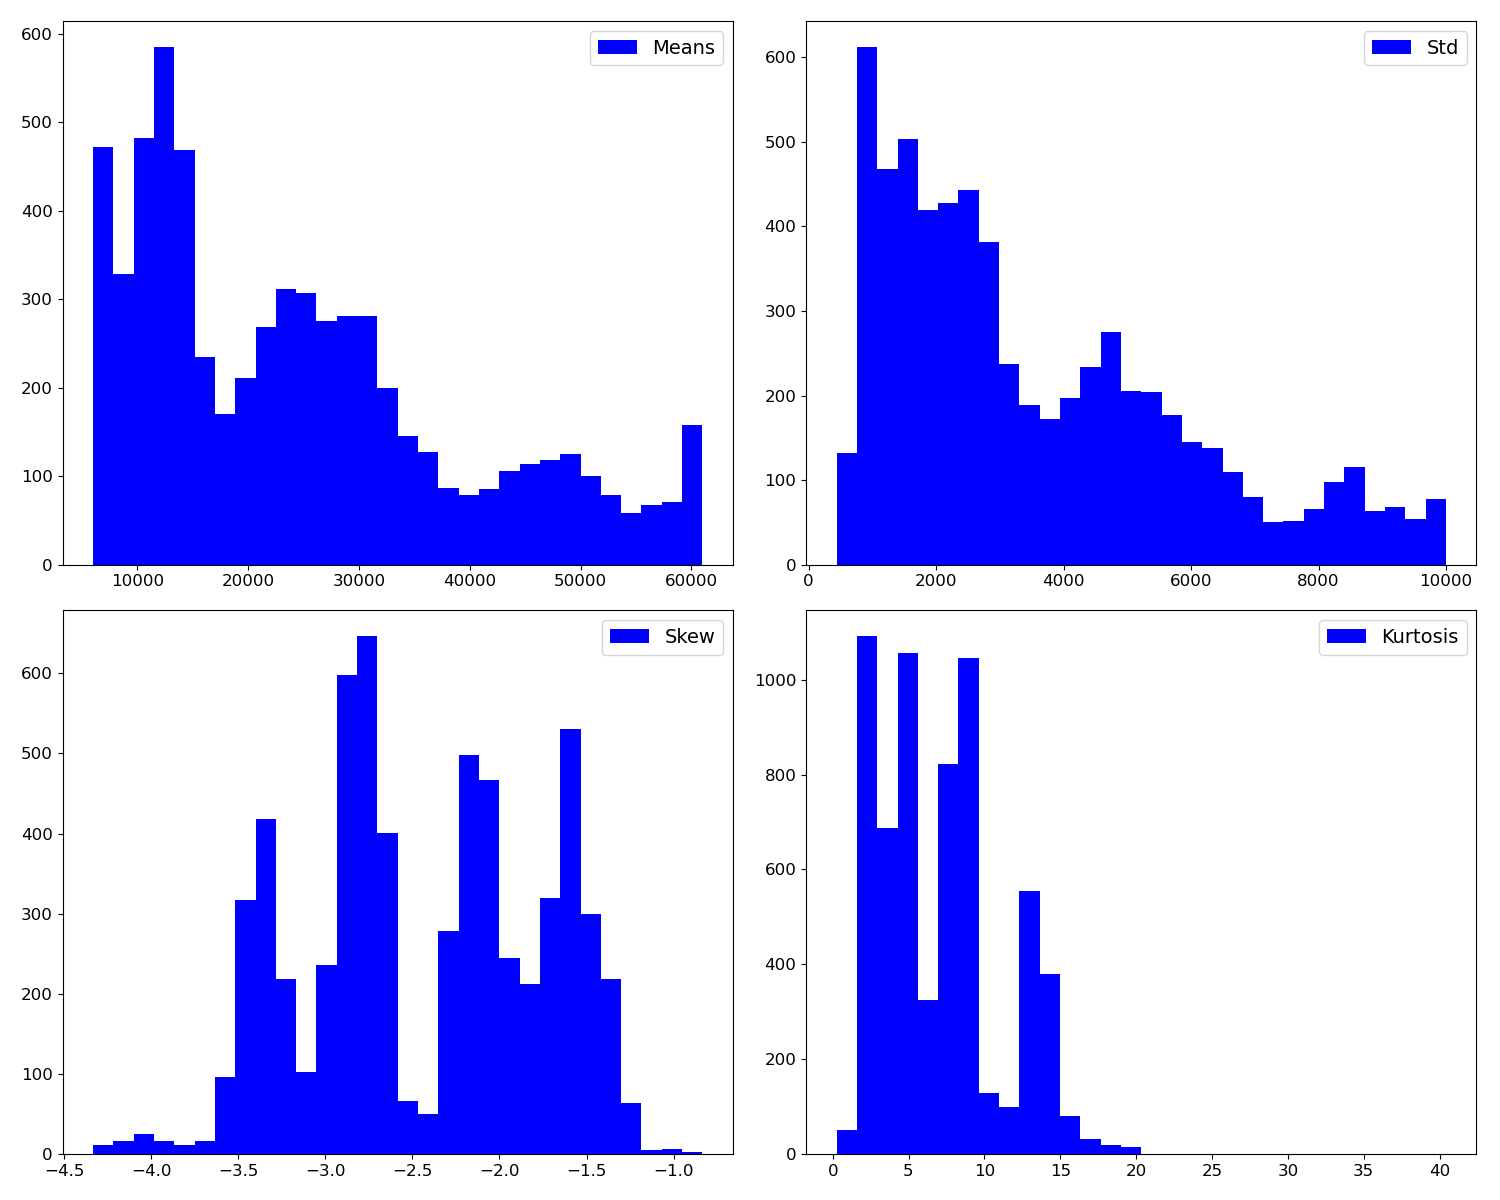
\includegraphics[scale=0.4]{images/flatdisplimssd10000.png}
\end{center}   
\caption{This figure is the same data as for Fig. \ref{fig:flatdisplims} except
additionally flat files with standard deviations over 10,000 are omitted.
The skewness and kurtosis are not shown on a logarithmic scale as they are
distributed more evenly.} \protect\label{fig:flatdisplimssd10000}
\end{figure}
\clearpage

\subsubsection{Creation of alternative master flat files}
\protect\label{seciion:altmasters}

Having determined appropriate alternative criteria, it was appropriate to
consider the construction of alternative master flat files.

The existing master flat files are composed of daily flat files taken from the
preceding month and might consist of files taken 30 days from the relevant
observation date. As with the alternative master bias files as described in
Section \ref{section:dailybiasfiles}, a rolling ``window'' of daily flat files
is used to construct a master flat file tailored to the observation date. 

The existing master flat files were composed by taking the median value for each
pixel from the selected daily flat files and then normalising. As the daily flat
files are taken in groups of three as the light fades but taking the median will
ignore all but the middle set in each case. The benefit of having flat fields
with brighter frames will be lost as well as the darkest flat field frames
(although care must be taken, the signal to noise is lowest on these).

The approach selected was to normalise first and, as the results are ratios
close to 1, combine with a geometric mean.

Unfortunately, this at first presented a problem as the pixels, after
subtraction of the bias files, become zero or negative in some cases, mostly
associated with the lower illumination files, as has also been noted in the
observation files. It is, of course, not possible to calculate a geometric mean
of a sample containing negative or zero values.

However this was first undertaken using the selection criteria used in the
creation of the master flat files, using frames with a mean pixel count between
5,000 and 50,000\footnote{As discussed in section \ref{section:flatselection}
above, the additional skewness and kurtosis restrictions are ignored here.}.

A number of strategies were tried to eliminate flat field images yielding
negative values after subtraction of the master bias images (or alternative
master bias images). These were:

\begin{itemize}
  \item Revision of the selection criteria for flat files as suggested by the
  work in Section \ref{section:flatselection} to those files with means between 6,000 and 61,000
  pixels (the lower limit here being more important for these purposes).
  However this was not completely effective for flat files for the \texttt{z}
  filter. There remained some flat files in 2018, mainly May that still gave
  negative pixels. If the lower limit of means is set to 7,000 for the
  \texttt{z} filter, then the negative pixels are eliminated for the remaining
  files for that filter. However this loses approximately 50\% of the files.
  \item Trim 50 pixels from each edge of the flat field images, however this
  still leaves some flat files for the \texttt{z} filter yielding negative
  pixels.
  \item Eliminate any file with a minimum pixel value below 200 counts (this
  figure was arrived at by considering the mean pixel value over all daily bias
  files of 300). This would lose just over 1\% of all the daily flat files, but
  those would be the files with the poorest signal to noise ratio. Raising the
  threshold to 300 counts would lose just over 2\% of the files and did not
  appear to be necessary.
  \item Eliminate any file with a maximum pixel value above 65,000 counts where
  saturation is approached and the performance is more erratic. This would lose
  about 0.25\% of all the files except for those corresponding to the \texttt{z}
  filter, where 0.5\% of the files would be lost. In only about 5 cases, though
  the same files excluded by these restriction were not excluded by the
  previous restriction of the minimum values.
  \item Apply Gaussian smoothing to each of the daily flat files before
  subtraction of the bias files.
\end{itemize}

It was concluded that the selection criteria to work with for the daily flat
files, taking all these into account, was to restrict selection to the
following.

\begin{itemize}
  \item Frames having mean pixel values to between 6,000 and 61,000.
  \item Frames having minimum pixel values over 200.
  \item Frames having maximum pixel values below 65,000
  \item Frames with standard deviations on pixel values below 10,000.
  \item No consideration of skewness or kurtosis.
\end{itemize}

\textit{I now realise I can do better, including more low light flat files, if
I apply the bad pixels masks first.}

The proportions of daily flat files thereby selected by filter are set out in
Table \ref{table:selectedflats}.

\begin{table}[!htbp]
\begin{center}
\begin{tabular}{lrrr} \hline
Filter & Original & Mean limits & Selected limits\\\hline
\texttt{g} & 30.825 & 75.372 & 69.577\\
\texttt{i} & 36.298 & 68.813 & 63.602\\
\texttt{r} & 36.854 & 66.365 & 66.345\\
\texttt{z} & 58.379 & 60.772 & 60.310\\
\hline
Overall & 40.589 & 67.830 & 64.958\\

\hline
\end{tabular}
\end{center}
\caption{This shows the percentages of daily flat files eligible for selection
for each filter (first column) using the original criteria (second column),
just changing the range of means (third column) and the criteria finally
selected, limiting flat fields with maximum pixel values less than 65,000,
minimum values greater than 200 and standard deviation less than 10,000.}.
\protect\label{table:selectedflats}
\end{table}
\clearpage

\subsection{Hotspots or defective pixels}
\protect\label{section:hotspots}

A study was undertaken of all the files, flat files, bias files and observation
files to determine whether any pixels in the CCD array could be counted as
``bad'' or unresponsive, had particularly high mean values or large standard
deviation. The literature varies somewhat on how bad pixels are defined or
determined.

Of recent papers, \citet{allers20} define bad pixels as ``dead'' pixels or pixels
with an uncertainty in the flat fields of over 10\%. In \citet{piskunov20} bad
columns in the CCD used are first identified and eliminated and then an
iterative procedure is adopted to effectively assign weights to each pixel. In
\citet{bongiovanni19} a procedure based on constructing two composite flat
fields from low and high counts and regarding as bad the pixels where the ratios
differ by more than 15\%. In \citet{belli18} a bad pixel mask is constructed by
selecting pixels in the flat fields with very low counts and those in the dark
frames with very high counts (but the criteria for ``low'' and ``high'' counts
in those files are not defined). In \citet{briesemeister18} pixels in the
constructed flat fields with values less than 0.5 or greater than 1.5 are
considered to be bad. A comprehensive study of types of bad pixels is shown in
the recently-published \citet{maslennikova20}.

There were no examples which could be found of ``dead'' pixels, i.e. ones which appeared to be completely
unresponsive at all times, however some are particularly noisy, some are
non-linear and some perform badly, in that they ``drop out'' and give a low
reading from time to time.

There are three types of poor-quality pixels which are catered for here.

\begin{enumerate}
\item Particularly noisy pixels, which can be identified from the bias files.
\item Pixels which give seemingly random values, totally out of line with their
neighbours, usually a low value.
\item Pixels which are non-linear or which behave significantly differently from
their neighbours.
\end{enumerate}

\subsubsection{Possible unreliable pixels shown on bias files}
\protect\label{section:badpixbias}

The mean and standard deviation of each pixel on the CCD actually used for the
observations was made by taking all the daily bias files, eliminating those with
pixel values below 200 counts or above 5,000 counts (this eliminated 12\% of the files for the \texttt{g} filter, 13\% of the files for the\texttt{i} filter,
and 4\% for the \texttt{r} and \texttt{z} filters, 92\% overall) and locating
each pixel on the CCD.
In Fig. \ref{fig:mean_allbiaslim250_5000} is shown the mean values over the whole of the
CCD and in \ref{fig:std_allbiaslim250_5000} the standard deviations.

\begin{figure}[!htbp]
\begin{center}
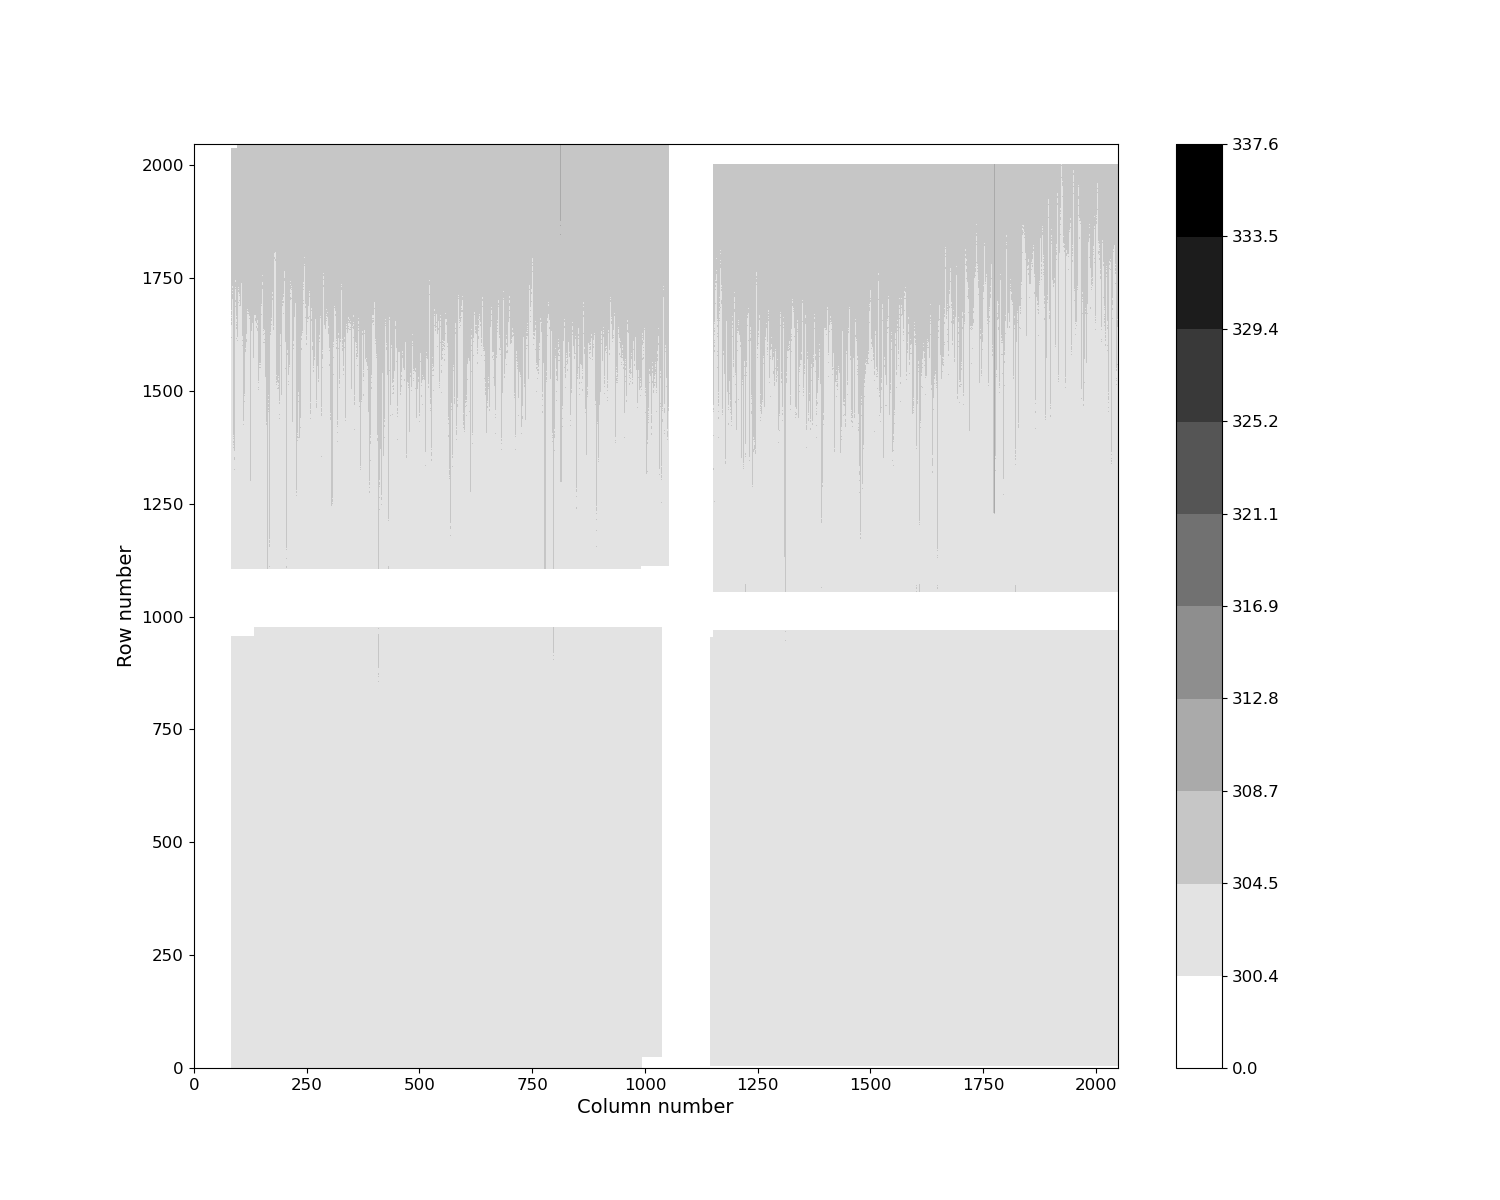
\includegraphics[scale=0.3]{images/mean_allbiaslim250_5000.png}
\end{center}   
\caption{This figure shows the distribution of mean values of the bias counts
for each pixel on the CCD obtained by taking all the daily bias files, ignoring
those with minimum values below 200 or above 5,000. The four areas used are the
same as in all the other figures, i.e. top left is that used by the \texttt{i}
filter, the top right corresponds to the \texttt{g} filter, the bottom left
that used by the \texttt{z} filter and the bottom right that used by the
\texttt{r} filter.} \protect\label{fig:mean_allbiaslim250_5000}
\end{figure}

\begin{figure}[!htbp]
\begin{center}
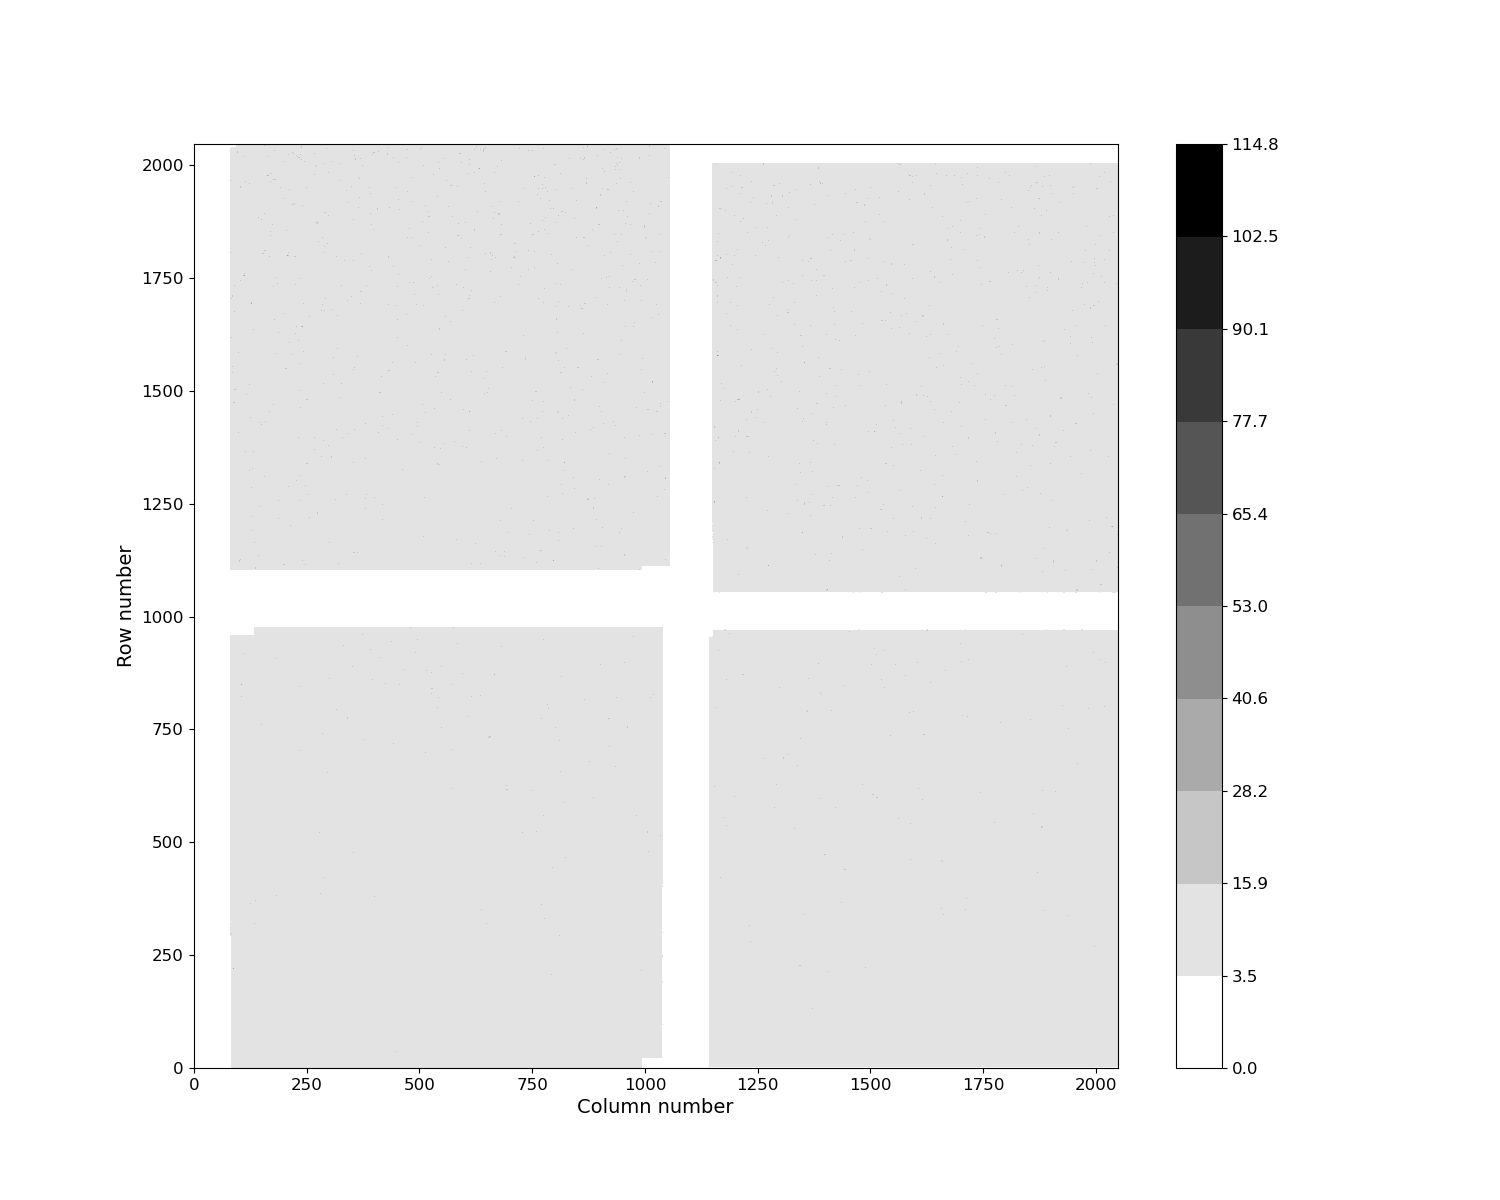
\includegraphics[scale=0.3]{images/std_allbiaslim250_5000.png}
\end{center}   
\caption{This figure shows the distribution of standard deviations of the
bias counts for each pixel on the CCD obtained by taking all the daily bias files, ignoring
those with minimum values below 200 or above 5,000. The four areas used are the
same as in all the other figures, i.e. top left is that used by the \texttt{i}
filter, the top right corresponds to the \texttt{g} filter, the bottom left
that used by the \texttt{z} filter and the bottom right that used by the
\texttt{r} filter.}
\protect\label{fig:std_allbiaslim250_5000}
\end{figure}
\clearpage

It can be seen that the noise level in individual pixels is spread evenly, but
the base bias level of the pixels holds to a consistent pattern which mostly
affects the \texttt{i} and \texttt{g} filters at the top of the images. The
columns (by which readouts are taken from the CCD are easily recognisable in the daily bias files, but the
rows not nearly so much. It is perhaps unfortunate that this applies to the
\texttt{g} filter as the number and brightness of the objects is generally
better for this filter.

\subsubsection{Pixels with random or significantly out-of-line values}
\protect\label{section:randpixels}

In Fig. \ref{fig:flatdemobadpix} is shown a daily flat file and in Fig.
\ref{fig:flatdemozoom} part zoomed in to show pixels which are significantly out
of line with the surrounding pixels.

%image_display.py --grey flatdisp F:122012
\begin{figure}[!htbp]
\begin{center}
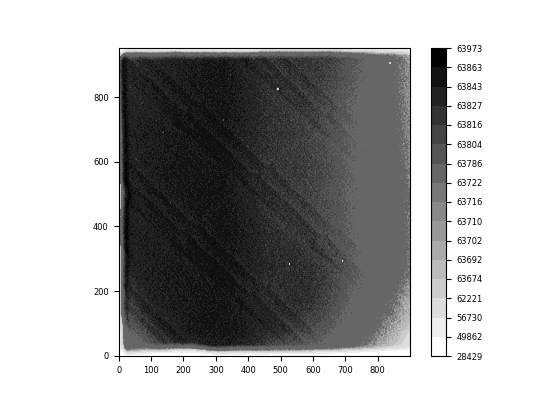
\includegraphics[scale=1]{images/flatdemo2022.png}
\end{center}   
\caption{This shows the brighest daily flat file made on 24 May 2022 at 22:04:37
for the \texttt{g} filter. It will be seen that that there are various dark
points (in this inverse image appearing as bright points) where the pixels are
signficantly lower then their neighbours.} \protect\label{fig:flatdemobadpix}
\end{figure}

\begin{figure}[!htbp]
\begin{center}
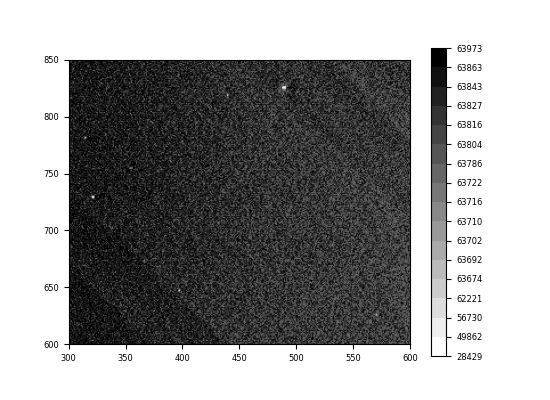
\includegraphics[scale=1]{images/flatdemo2022z.png}
\end{center}   
\caption{This is a close-up of the daily flat file depicted in Fig.
\ref{fig:flatdemobadpix} showint part of the image particularly affected by
unreliable pixels.} \protect\label{fig:flatdemozoom}
\end{figure}

These pixels are eliminated from consideration and where they overlap with
objects are replaced by the mean of the surrounding 8 pixels.\footnote{In just
a few cases consecutive pixels are eliminated in this way, usually in columns
on the array, and this may be 6 or 7 adjacent pixels.}

\subsubsection{Unreliable pixels}
\protect\label{section:unreliable pixels}

There are some pixels which some of the time behave normally but occasionally
are unresponsive, resulting in some negative values after the bias value is
removed.

It is possible to weed these out by first excluding the consistently unreliable
pixels described in Section \ref{section:randpixels} above, which are easy to
detect, having uncertainty over 5 standard deviations, and then excluding pixels
as described in \citet{allers20}, however by limiting the exclusion to 15\%
rather than 10\%.

It might be acceptable to include these pixels when they behave normally, but it
does not appear to be worthwhile at the present time.

\subsubsection{Total bad pixel statistics}
\protect\label{section:totalbadpix}

\textit{I'm going to display totals for bad pixels for each filter before and
after reconfiguration in March 2019 and also showing any overlaps.}

\subsection{Results after callbartion revisions}
\protect\label{section:postcalibration}

\textit{I need to write this section to show the improvements made to the
displays in Fig. \ref{fig:initgexample} etc and elimination of negative pixels
via these efforts. The full treatment of bad pixels probably means that I can
include more daily flat files excluded previously due to negative pixels.}

\clearpage
 
% \subsection{Flat files}
% \protect\label{section:flatfiles}
% 
% Two kinds of flat file are provided, a set of daily flat files for each of the
% filters, typically 2 or 3 each day for each of the 4 visible light filters \textbf{g},
% \textbf{i}, \textbf{r} and \textbf{z} and for gains of 1 and 4 and the monthly
% master flat files, consisting of a composite of the daily flat files for the
% month.
% 
% \subsubsection{Daily flat files}
% \protect\label{section:dailyflatfiles}
% 
% The daily flat files, after the end of 2013, which precedes the first of the
% observations, are taken with an exposure time of 1 second. Some have a gain of
% 4.4, in line with the gain applied to some of the other observations, but in
% this report only the flat files with a gain of 1 are considered as all the
% observations of the 3 target stars were taken with a gain of 1.
% The master flat files are only taken from these. Usually (but not always) three
% flat files are taken will decreasing light. In Fig. \ref{fig:giflat} are shown
% typical daily flats for the \texttt{g} and \texttt{i} filters, and in Fig.
% \ref{fig:rzflat} are shown similar ones for the \texttt{r} and \texttt{z}
% filters.
% 
% \begin{figure}[!htbp]
% \begin{center}
% %\includegraphics[scale=.4]{images/giflat.png}
% \end{center}   
% \caption{These are examples of two typical daily flat files for the \texttt{g}
% and \texttt{i} filters.}
% \protect\label{fig:giflat}
% \end{figure}
% 
% \begin{figure}[!htbp]
% \begin{center}
% %\includegraphics[scale=.4]{images/rzflat.png}
% \end{center}   
% \caption{These are examples of two typical daily flat files for the \texttt{r}
% and \texttt{z} filters.}
% \protect\label{fig:rzflat}
% \end{figure}
% Rows and columns of the image containing zero pixels were removed from the
% images before analysis. These values are replaced by \texttt{NaN} in the master
% flat files and correspond to invalid pixels. They cannot be used in computations
% as the pixels in the object are divided by the same pixel corresponding flat
% file which would entail division by zero.
% 
% It was of concern that many of the daily flat files had pixels which were vary
% close to saturation. in some cases they were clearly saturated, but none of the
% master flat files appeared to incorporate the daily flat files with definitely
% saturated pixels. In Table \ref{table:satpix} is shown the proportion of
% nearly saturated pixels in flat files for each filter.
% 
% \begin{table}[!htbp]
% \begin{center}
% \begin{tabular}{lrrr} \hline
% Filter & Flat files & Saturated & Over 50\%\\\hline
% g & 3,679 & 29.49 & 22.34 \\
% i & 3,679 & 32.37 & 27.43 \\
% r & 3,680 & 32.66 & 28.12 \\
% z & 3,680 & 0.92 & 0.60 \\\hline
% Overall & 14,718 & 23.86 & 19.62\\
% \hline
% \end{tabular}
% \end{center}
% \caption{Breakdown of daily flat files by filter up to August 2019 showing
% number, percentage with nearly saturated pixels present and percentage with over
% 50\% saturated pixels (in many cases this was over 90\% and occasionally 100\%).}
% \protect\label{table:satpix}
% \end{table}
% 
% \subsubsection{Linearity of CCDs}
% 
% It might be reasonable to expect that if the CCDs are linear, then the standard
% deviation of the values in the daily flat files would rise in proportion to the
% mean values in the daily flat files. In Fig. \ref{fig:ffcorr} is shown how this
% correlates for the four filters.
% 
% \begin{figure}[!htbp]
% \begin{center}
% %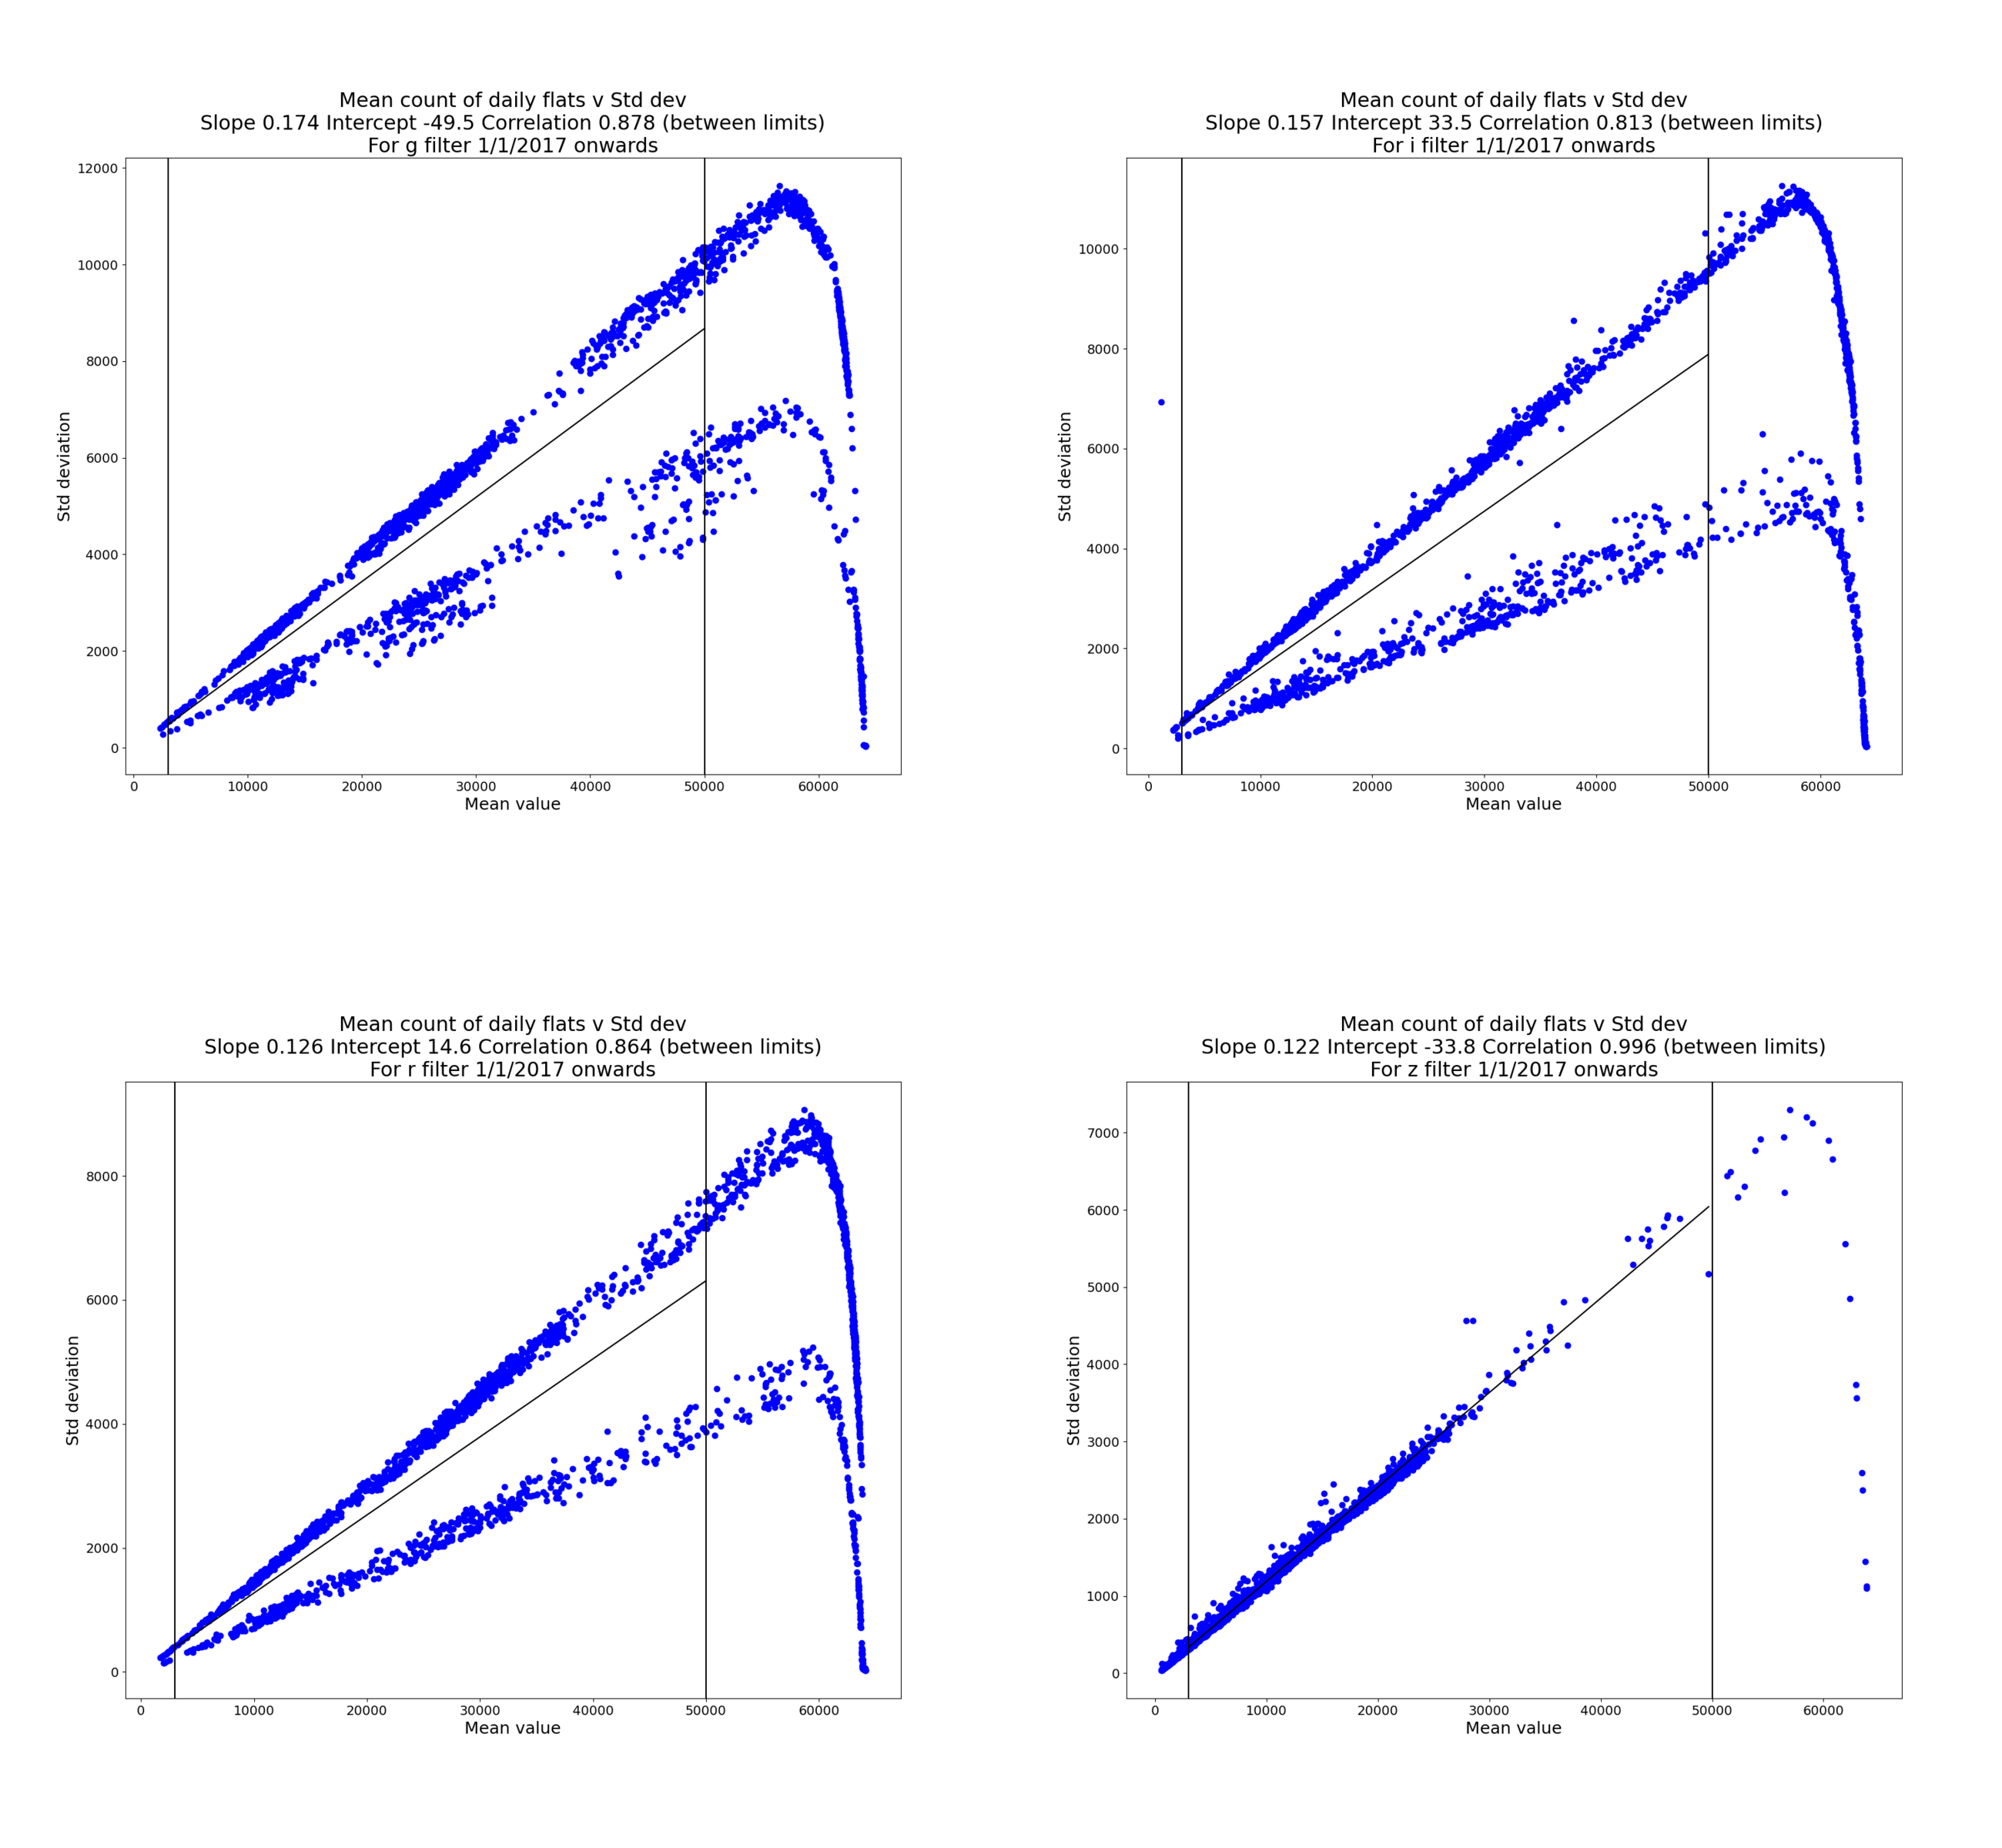
\includegraphics[scale=0.2]{images/corr.png} \\
% \end{center}   
% \caption{This figure shows how the standard deviation of the values in the
% daily flat files corresponds to the four filters. In the top is shown the
% results for the \texttt{g} filter, the bottom left shows the \texttt{r} filter,
% the top right shows the results for the \texttt{i} filter and the bottom right
% shows the results for the \texttt{z} filter. The black line shows the best fit
% slope in each case. The black vertical lines show the upper and lower limits of
% the selection originally used in the master flat files, i.e. mean between 5,000
% and 50,000. Calculation of the best fit slope is restricted to values between
% those limits.}
% \protect\label{fig:ffcorr}
% \end{figure}
% 
% The master flat files are built from flat files with means between 5,000 and
% 50,000, which would appear to be a reasonable choice, the linearity drops off
% dramatically as saturation is reached in all cases.
% %\
% \subsubsection{Master flat files}
% \protect\label{section:masterflatfiles}
% 
% The master flat files consist of median values of the incorporated daily flat
% files, the header indicating which ones are considered.
% 
% Invalid pixel values are represented by \texttt{Nan} and rows and columns
% containing these values are trimmed from the images, both for the flat files
% themselves, and also for the corresponding bias and observations files.
% 
% The program used to create the master flat files selects daily flat files with a
% mean value between 5,000 and 50,000 \textbf{and} with a negative skew and
% kurtosis less than 7. It seemed probable that this latter restriction was a
% mistake and ``\textbf{or}'' was intended
% 
% It would appear to the author that the upper limit is too great and several
% files with saturated pixels are included, using the median pixel value will
% exclude these, but this creates a difficulty in that as 3 daily flat files are
% taken from the sky before observations start, effectively the middle one is
% taken in each case by the median.
% 
% It appeared that each daily flat file should
% be normalised first and the results combined, so a procedure to create
% alternative master flat files was devised. This turned out to be compromised by
% the extreme values in the bias files, which made some of the pixel values
% negative in the daily flat files before normalisation. The issues identified in
% Section \ref{section:hotspots} will have to be properly addressed in order to
% make progress here. The reason that the original master bias files were not
% affected by the negative pixel problem is that they were combined, with much
% higher individual pixel values, before normalisation not afterwards. The negative
% pixel values occur when the lowest light level daily flat file has the bias
% value subtracted before normalisation.
% 
% It was noticed that there was a computational error in the calculation of the
% mean, standard deviation and other parameters in the master flat files and these
% had to be discarded in any event. As the daily flat files change somewhat over
% time reliance on a master flat file possibly
% 30 days removed from the observations to which it relates would seem
% inappropriate and a procedure of ``rolling'' master flat files centred on the
% observation dated was adopted, but this cannot be proceeded until the problem of
% negative pixels in the daily flat files is resolved.

\subsubsection{Accuracy}
\protect\label{section:accuracy}

\textit{This probably wants moving somewhere else to a later section on
modifications to the REM telescope.}

Combination of daily bias values clearly improves the accuracy. The median
pixel value for all of the bias files for all of the filters is approximately
300 with a standard deviation of about 7 for the individual files, 3 for where
all the daily ones for a given day are merged and 1 for the master bias files.

It seemed worth looking at whether any adjustments of the exposure times might
improve the accuracy, as many of the objects which might be used for reference
give an ADU count only just above the sky level. The exposure times currently
are 10 seconds for {\prox} and Ross 154 and 5 seconds for \bstar.

Table \ref{table:pixvals} is set out the maximum value in any of the observation
files for each target and each filter and the percentage of observation files in
which at least one pixel exceeds a give number of ADUs (this does not currently
take account of defective pixels or cosmics, but these would have negligible
effects on the results).

It is clear that some increase in exposure time, possibly up to 5 times or more
in the case of the \texttt{g} filter, would benefit the contrast, except
for the \texttt{i} filter results, which are generally too close to saturation.
The nature of the instrument, however, may not permit any different exposure
times to be made with different filters.

\begin{table}[!htbp]
\begin{center}
\begin{tabular}{|l|r|rrrr|} \hline
Filter & Max value & \% over 30,000 & \% over 40,000 & \% over 50,000 & \% over
60,000 \\\hline
 \multicolumn{6}{|c|}{\textbf{\bstar} exp 5 sec} \\\hline
\texttt{g} & 63,422 & 0.05 & 0.05 & 0.05 & 0.05 \\
\texttt{i} & 63,448 & 78.94 & 61.15 & 45.71 & 0.77 \\
\texttt{r} & 54,806 & 16.68 & 3.73 & 0.97 & 0.00 \\
\texttt{z} & 63,387 & 12.52 & 3.37 & 0.87 & 0.05 \\
\hline
\multicolumn{6}{|c|}{\textbf{\prox} exp 10 sec} \\\hline
\texttt{g} & 63,466 & 0.38 & 0.30 & 0.25 & 0.18 \\
\texttt{i} & 63,457 & 74.15 & 52.88 & 36.84 & 4.03 \\
\texttt{r} & 63,425 & 0.60 & 0.10 & 0.09 & 0.08 \\
\texttt{z} & 63,456 & 25.38 & 11.64 & 5.47 & 0.16 \\
\hline
\multicolumn{6}{|c|}{\textbf{Ross 154} exp 10 sec} \\\hline
\texttt{g} & 63,453 & 0.41 & 0.35 & 0.28 & 0.22 \\
\texttt{i} & 63,452 & 76.71 & 57.35 & 39.25 & 2.16 \\
\texttt{r} & 63,268 & 7.99 & 2.38 & 0.93 & 0.11 \\
\texttt{z} & 63,447 & 8.33 & 2.14 & 0.45 & 0.04 \\
\hline
\hline
\end{tabular}
\end{center}
\caption{This figures shows the maximum ADU values of any pixel in any of the
observation files for each of the 3 {\rdwarf} targets for each filter. The
following columns show the percentage of pixels in each case which are above
30,000, 40,000, 50,000 and 60,000.}.
\protect\label{table:pixvals}
\end{table}
\clearpage

% \subsection{Analysis of images}
% \protect\label{section:analimages}
% 
% \textbf{Please note that since I realised that the master flat files are not
% normalised as Luciano told me I'll have to redo all this. The results within
% each month are consistent but not with other months. Also with the flat files
% properly normalised some of the images will have greater contrast.}
% 
% \subsubsection{Intensity comparison}
% \protect\label{section:intcomp}
% 
% As a first attempt to study the data, the ADU count was taken, specifically the
% net after applying the flat and bias files of the target in all the images in which it was available.
% The target was found in all of the images, apart from in a few of the
% \textbf{g}, \textbf{i} and \textbf{r} visible light filters,
%, as shown in Table
%\ref{table:occtb} below.

%Plotting light curves of the intensities obtained in this way yields Fig.
% \ref{fig:allall}.
%Binning the intensities together into a single day gave
%Fig. \ref{fig:allbin}, the error bars indicate the spread over a single day.

%I plotted
%periodograms, as shown in Fig. \ref{fig:pgrams}. Despite the crudeness of the
%data, it is noticeable that there are peaks close to the rotation periods of
% the order of 150 days referred to in \citet{suarezmascareno15} and \citet{toledopadron18}.

% \begin{figure}[!htbp]
% \begin{center}
% 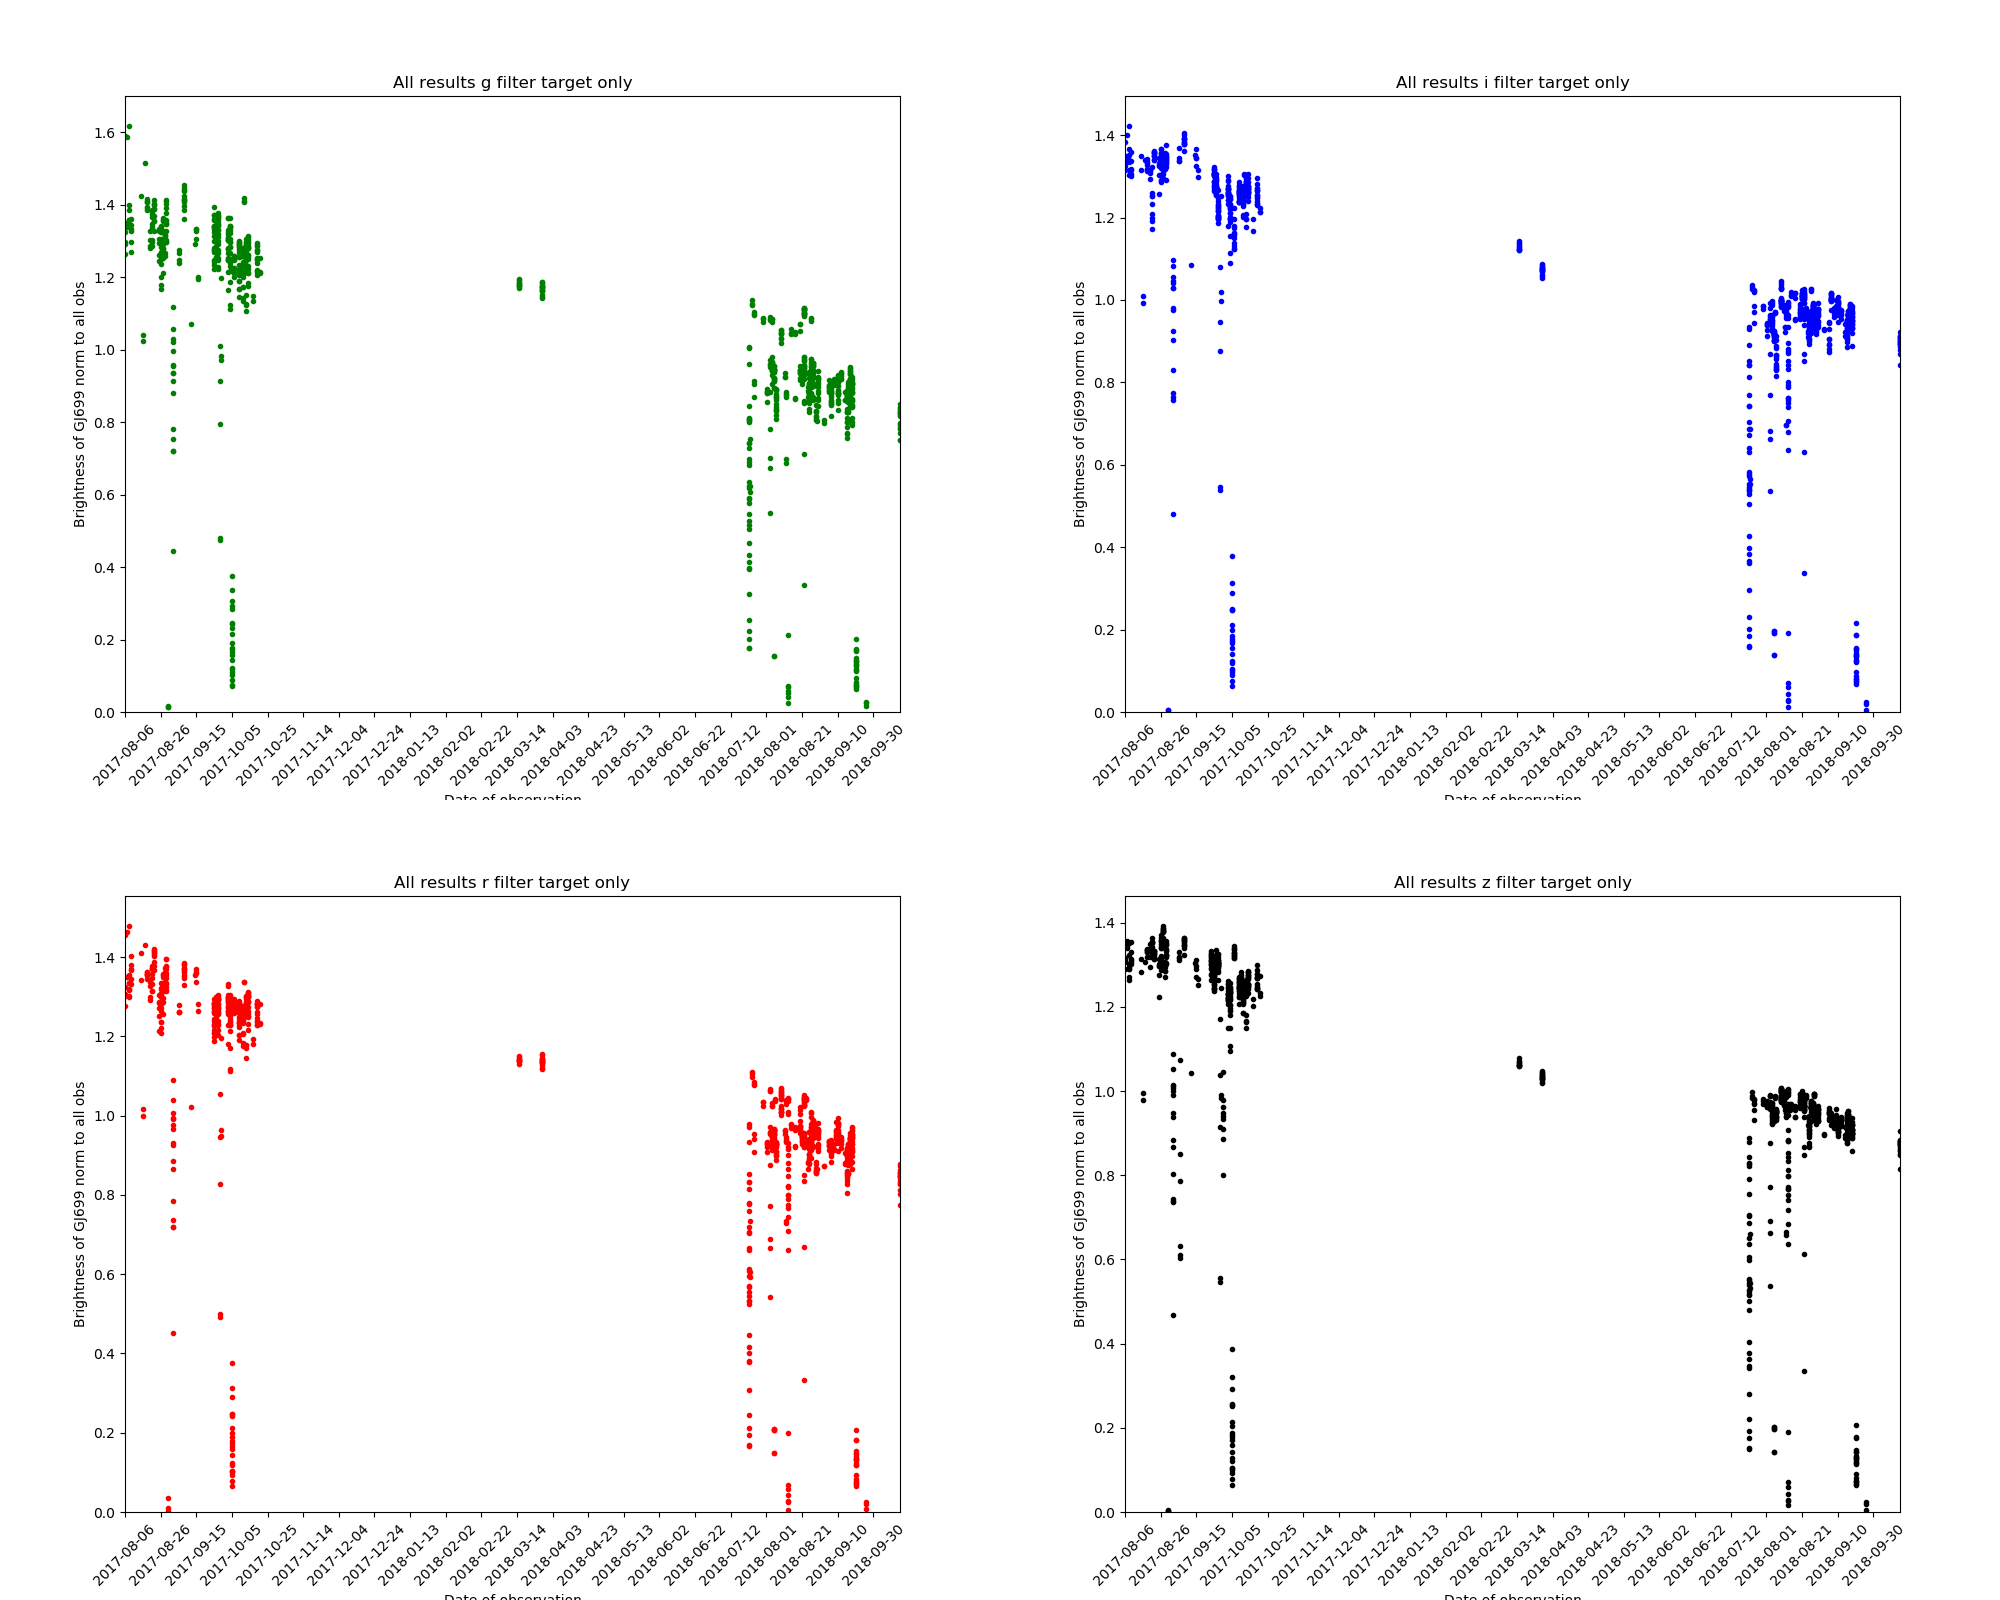
\includegraphics[scale=0.25]{images/allall.png} \\
% \end{center}   
% \caption{This shows the flux for the target, \bstar, for each of the four visible light filters. This takes the total
%   ADU count only}
%   \protect\label{fig:allall}
% \end{figure}
% 
% \begin{figure}[!htbp]
% \begin{center}
% 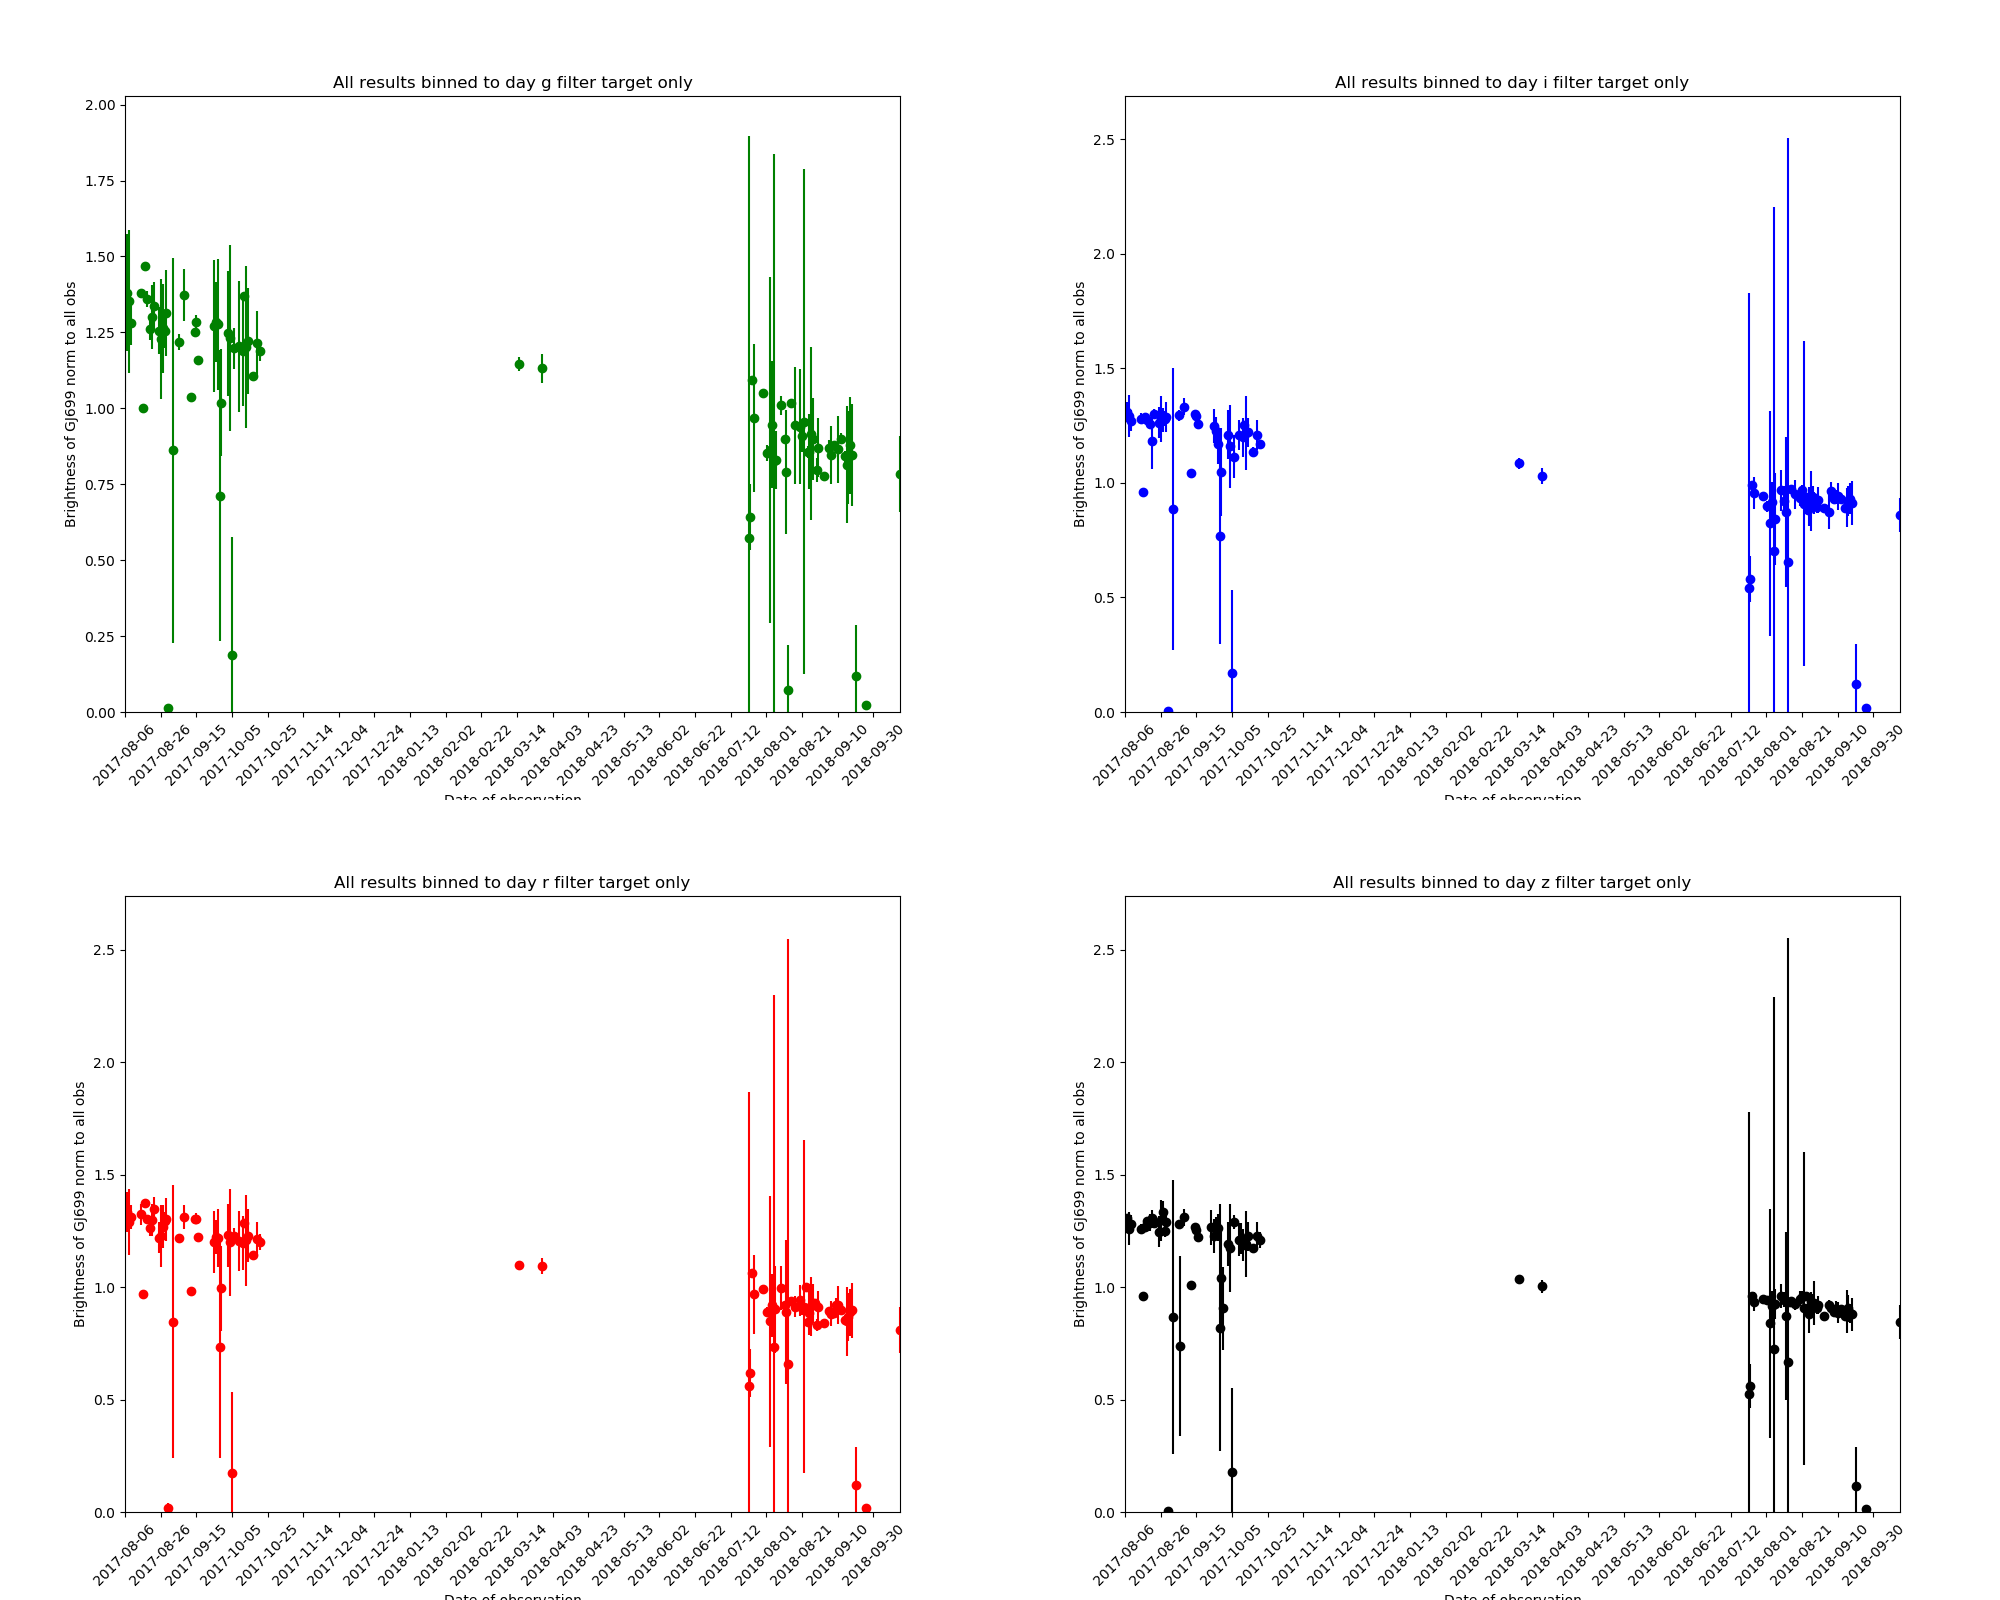
\includegraphics[scale=0.25]{images/allbin.png} \\
% \end{center}   
% \caption{This shows the flux for the target, \bstar, for each of the four visible light filters and binned to a single day. Error bars are show to indicate the spread of intensities over a single day.}
%   \protect\label{fig:allbin}
% \end{figure}

%\begin{figure}[!htbp]
%\begin{center}
%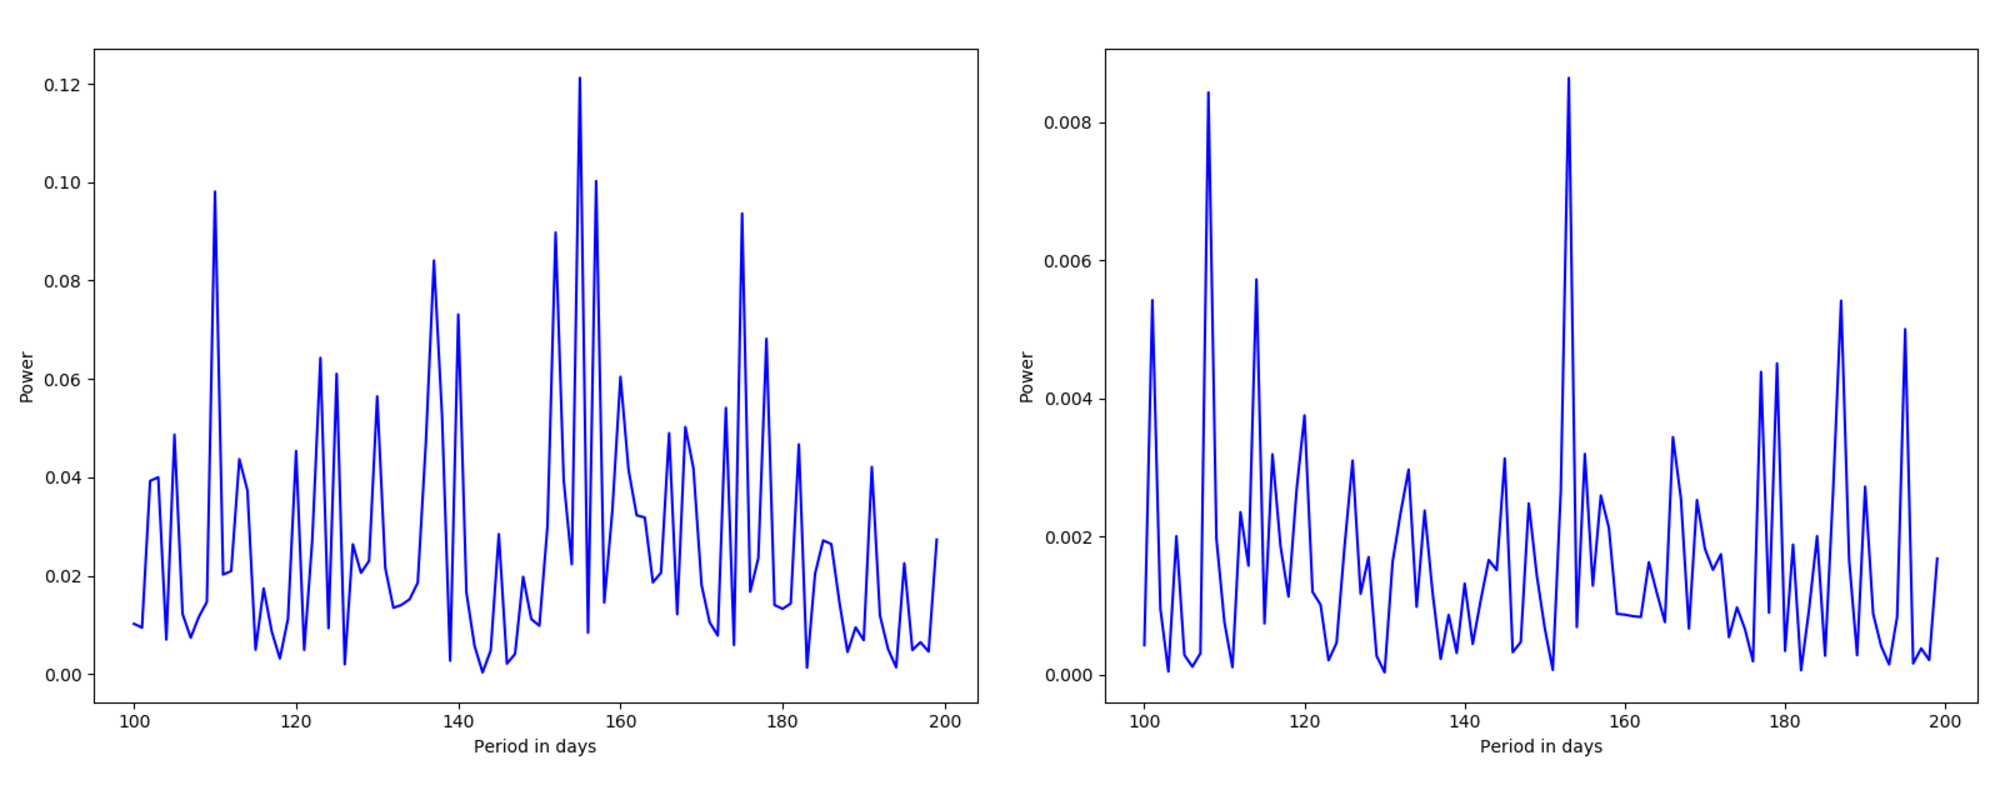
\includegraphics[scale=0.25]{images/pgrambunb.png} \\
%\end{center}   
%\caption{This displays periodograms derived from the binned (Fig.
% \ref{fig:allbin}) and unbinned (Fig. \ref{fig:allall}) light curves for the \textbf{r} filter.}
%  \protect\label{fig:pgrams}
%\end{figure}

% It is accepted that this initial treatment is crude. Serious work needs to be done on correction for air mass,
% which for a few observations, where they are spread over a period of several hours,
% can be quite large, and to more accurately discard as unacceptable images with large or very variable sky levels.
% There are some currently inexplicable variations, for
% example the to images in Fig. \ref{fig:tyeg} give radically different ADU counts despite being taken two minutes apart
% with same exposure time and other parameters.
% 
% \begin{figure}[!htbp]
% \begin{center}
% 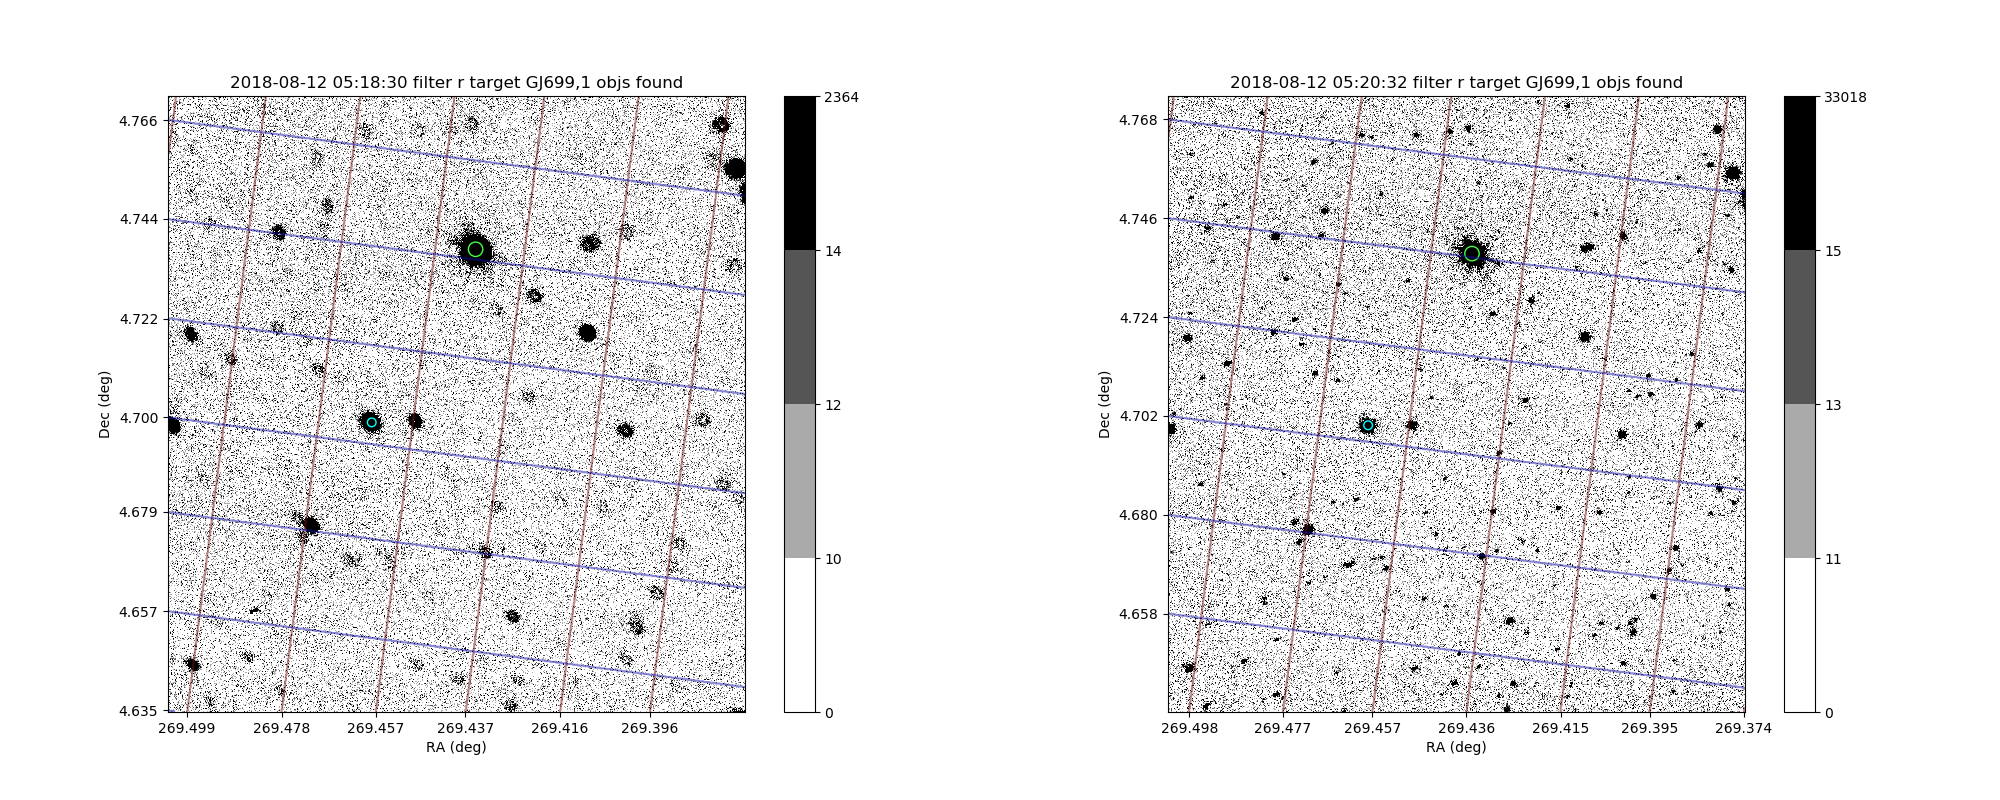
\includegraphics[scale=0.25]{images/tyeg.png}
% \end{center}   
% \caption{These images show an example of where 2 images taken 2 minutes apart with the same exposure time gave different flux values.}
%   \protect\label{fig:tyeg}
% \end{figure}
% 
% \subsubsection{Reference Stars}
% \protect\label{section:refstars}
% 
% Rather than relying on the ``raw'' flux from the target star itself, it was
% considered that an approach based on identified reference stars found in a
% significant number of images.
% Ideally these should be as many as possible to ``smooth'' out errors and variations on the reference star. 
% Byy taking the ratio of the target star ADU count to the sum of the reference
% star ADUs, then we can hope to achieve results for intensity with the factors such air mass corrections factored out, This
% approach was taken in \citet{berry11} and would seem to involve least work, provided sufficient reference stars are
% consistently found.
% 
% The algoritm used to find objects was first to locate the target (there was
% usually a certain amount of error in the coordinates of the images) and then
% find prefeviously-known reference objects. The criterion for finding objects was to look for groups of pixels within a
% given scan aperture whose mean count was a given number of standard deviations
% (intially 3) from that of the sky level. If the result appeared to be one of
% the objects known already, the given reference object was deemed to have been
% found.

% In all cases the brightest objects were found in Simbad, 2MASS and SDSS
% to find objects in the vicinity of \bstar, obtaining the following stars as shown in Table \ref{table:reftimesfound}.
% Of the stars there, the types are unavailable apart from the most-frequently occurring one of
% TYC425-262-1, which is an A3V star (this is also reported as the most frequently found reference star in \citet{berry11}).
% 
% \begin{table}[!htbp]
% \begin{center}
% \begin{tabular}{llr} \hline
% Number & Object & Times found \\\hline
% 1 & TYC425-262-1 & 5,277 \\
% 2 & SDSS1237671695527248969 & 3,408 \\
% 3 & 2MASSJ17574653+0447466 & 3,297 \\
% 4 & SDSS1237668573088841773 & 840 \\
% 5 & TYC425-223-1 & 369 \\
% 6 & SDSS1237671695527249415 & 15 \\
% \hline
% \end{tabular}
% \end{center}
% \caption{This lists the identified reference objects near to {\bstar} and the number of times found in the available
%   data. Note that this data relates to images up to the end of October 2018.}
% \protect\label{table:reftimesfound}
% \end{table}
% 
% I decided to consider only the first 3 reference objects, which are labelled 1, 2 and 3 for convenience in the
% remainder of this report, as the appearances of the others were too infrequent to render them worthwhile.
% 
% \subsection{Classification of results}
% \protect\label{section:classresults}
% 
% The images presented challenges in various respects. The visible light images are all at different orientations and with
% the target in different places in the image, so not all the reference stars appear in all of the images. In some cases
% the reference stars are just not bright enough to rise sufficiently above the sky level.
% 
% \begin{table}[!htbp]
% \begin{center}
% \begin{tabular}{lrrrr}
% &Filter g&Filter i&Filter r&Filter z\\\hline
% Target not found&167&80&105&0\\
% No ref objs found & 84 & 1,003 & 53 & 1,085 \\\hline
% Obj 1 (with or without others) & 834 & 0 & 925 & 0 \\
% Obj 2 (with or without others) & 561 & 1 & 574 & 0 \\
% Obj 3 (with or without others& 526 & 0 & 573 & 0 \\
% Obj 1 only & 43 & 0 & 100 & 0 \\
% Obj 2 only & 0 & 1 & 1 & 0 \\
% Obj 3 only & 0 & 0 & 0 & 0 \\
% Objs 1 and 2 (with or without 3) & 561 & 0 & 573 & 0 \\
% Objs 1 and 3 (with or without 2) & 526 & 0 & 573 & 0 \\
% Objs 2 and 3 (with or without 1) & 296 & 0 & 321 & 0 \\
% Objs 1 and 2 only & 265 & 0 & 252 & 0 \\
% Objs 1 and 3 only & 230 & 0 & 252 & 0 \\
% Objs 2 and 3 only & 0 & 0 & 0 & 0 \\
% Objs 1,2 and 3 & 296 & 0 & 321 & 0 \\
% \hline
% \end{tabular}
% \end{center}
% \caption{This table shows the occurrences of the 3 main reference objects in each of the observations with or without
%   the others. The infrared images were omitted as no reference objects were found in any of them. Note however the lack
%   of occurrences of reference objects in the \textbf{i} and \textbf{z} filter images.}
% \protect\label{table:occtb}
% \end{table}
% 
% \subsection{Results from reference object comparisons}
% \protect\label{section:refobjres}
% 
% Repeating the light curve plots from Section \ref{section:intcomp}, this time as the ratio of the ADU count of the
% target to the sum of the first three reference objects, Fig.  \ref{fig:allref123} and Fig. \ref{fig:allref123bin} show
% the light curves for the \textbf{r} and \textbf{g} filters. Also shown in Fig. \ref{fig:ls123both} are periodograms
% derived from these light curves. Also shown in Fig \ref{fig:allref1}, Fig. \ref{fig:allref1bin} and Fig. \ref{fig:ls1both}
% are the corresponding results taking into account only the brightest of the reference objects, TYC425-262-1.
% 
% \begin{figure}[!htbp]
% \begin{center}
% 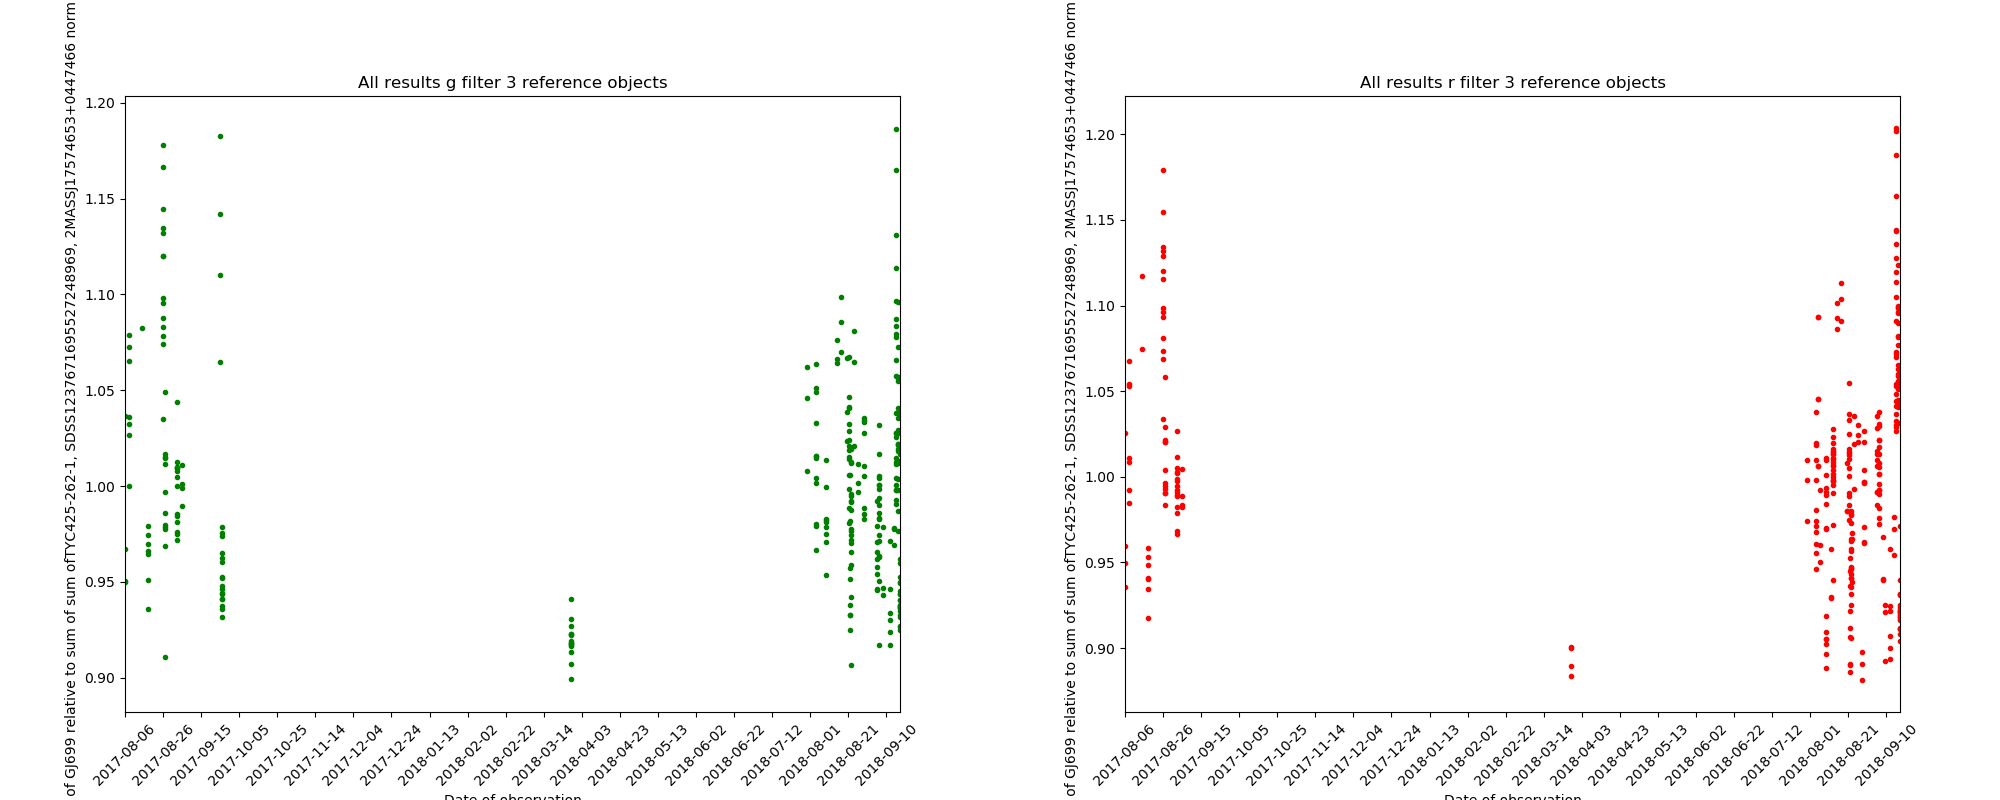
\includegraphics[scale=0.25]{images/allref123.png}
% \end{center}   
% \caption{This shows the ratio of the flux for the target, \bstar, to the 3 main reference objects for the \textbf{g} and
% \textbf{r} filters, plotted as green and red respectively.}
%   \protect\label{fig:allref123}
% \end{figure}
% 
% \begin{figure}[!htbp]
% \begin{center}
% 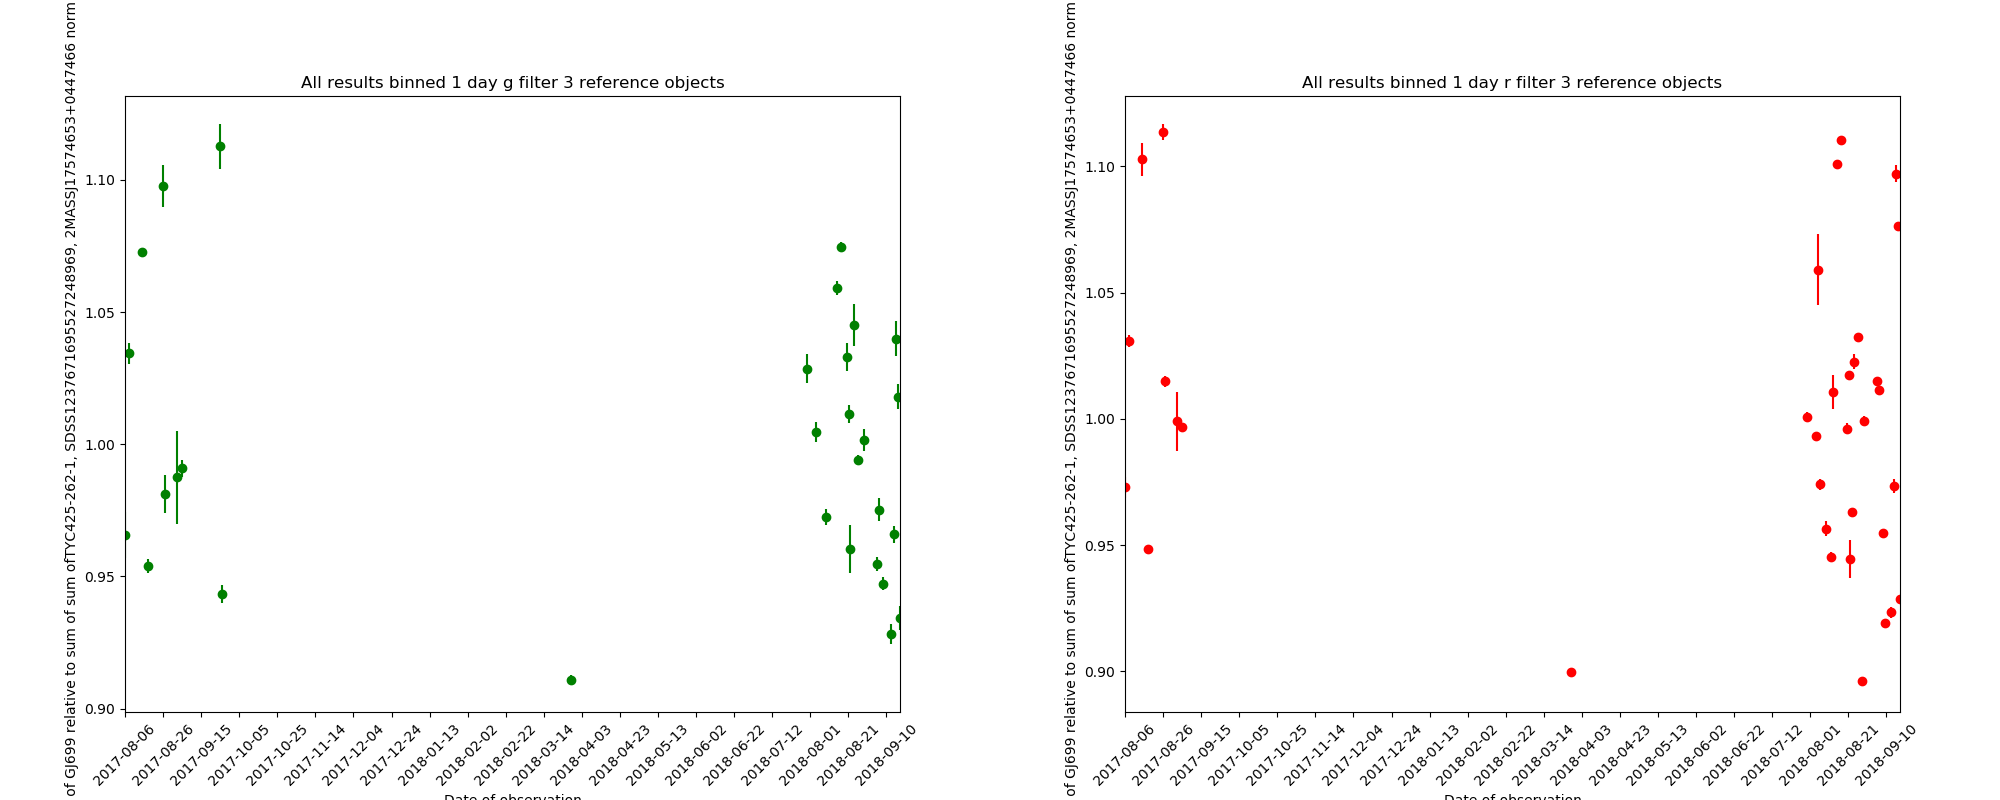
\includegraphics[scale=0.25]{images/allref123bin.png}
% \end{center}   
% \caption{This shows the ratio of the flux for the target, \bstar, to the 3 main reference objects as per Fig. \ref{fig:allref123} and binned to 1 day.}
%   \protect\label{fig:allref123bin}
% \end{figure}
% 
% \begin{figure}[!htbp]
% \begin{center}
% 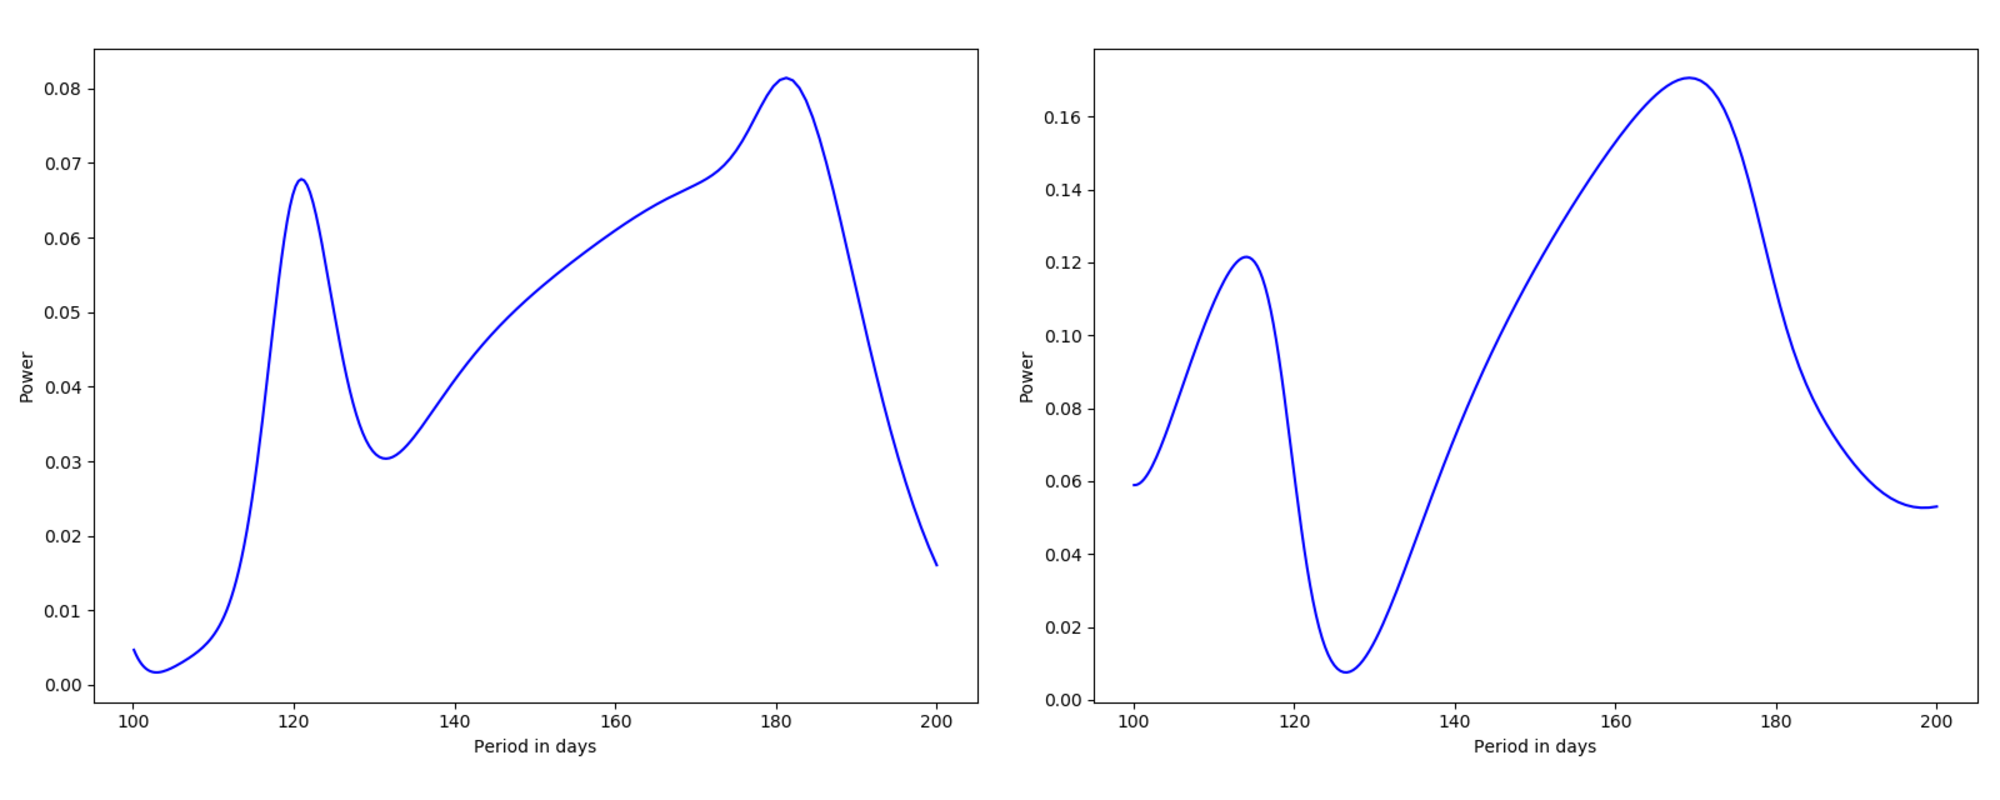
\includegraphics[scale=0.25]{images/ls123both.png}
% \end{center}   
% \caption{Periodograms obtained from Fig. \ref{fig:allref123}, left panel and Fig. \ref{fig:allref123bin} in right
%   panel. Only the \textbf{g} filter was used in this plot, the one from the \textbf{r} filter being almost identical.}
%   \protect\label{fig:ls123both}
% \end{figure}
% 
% \begin{figure}[!htbp]
% \begin{center}
% 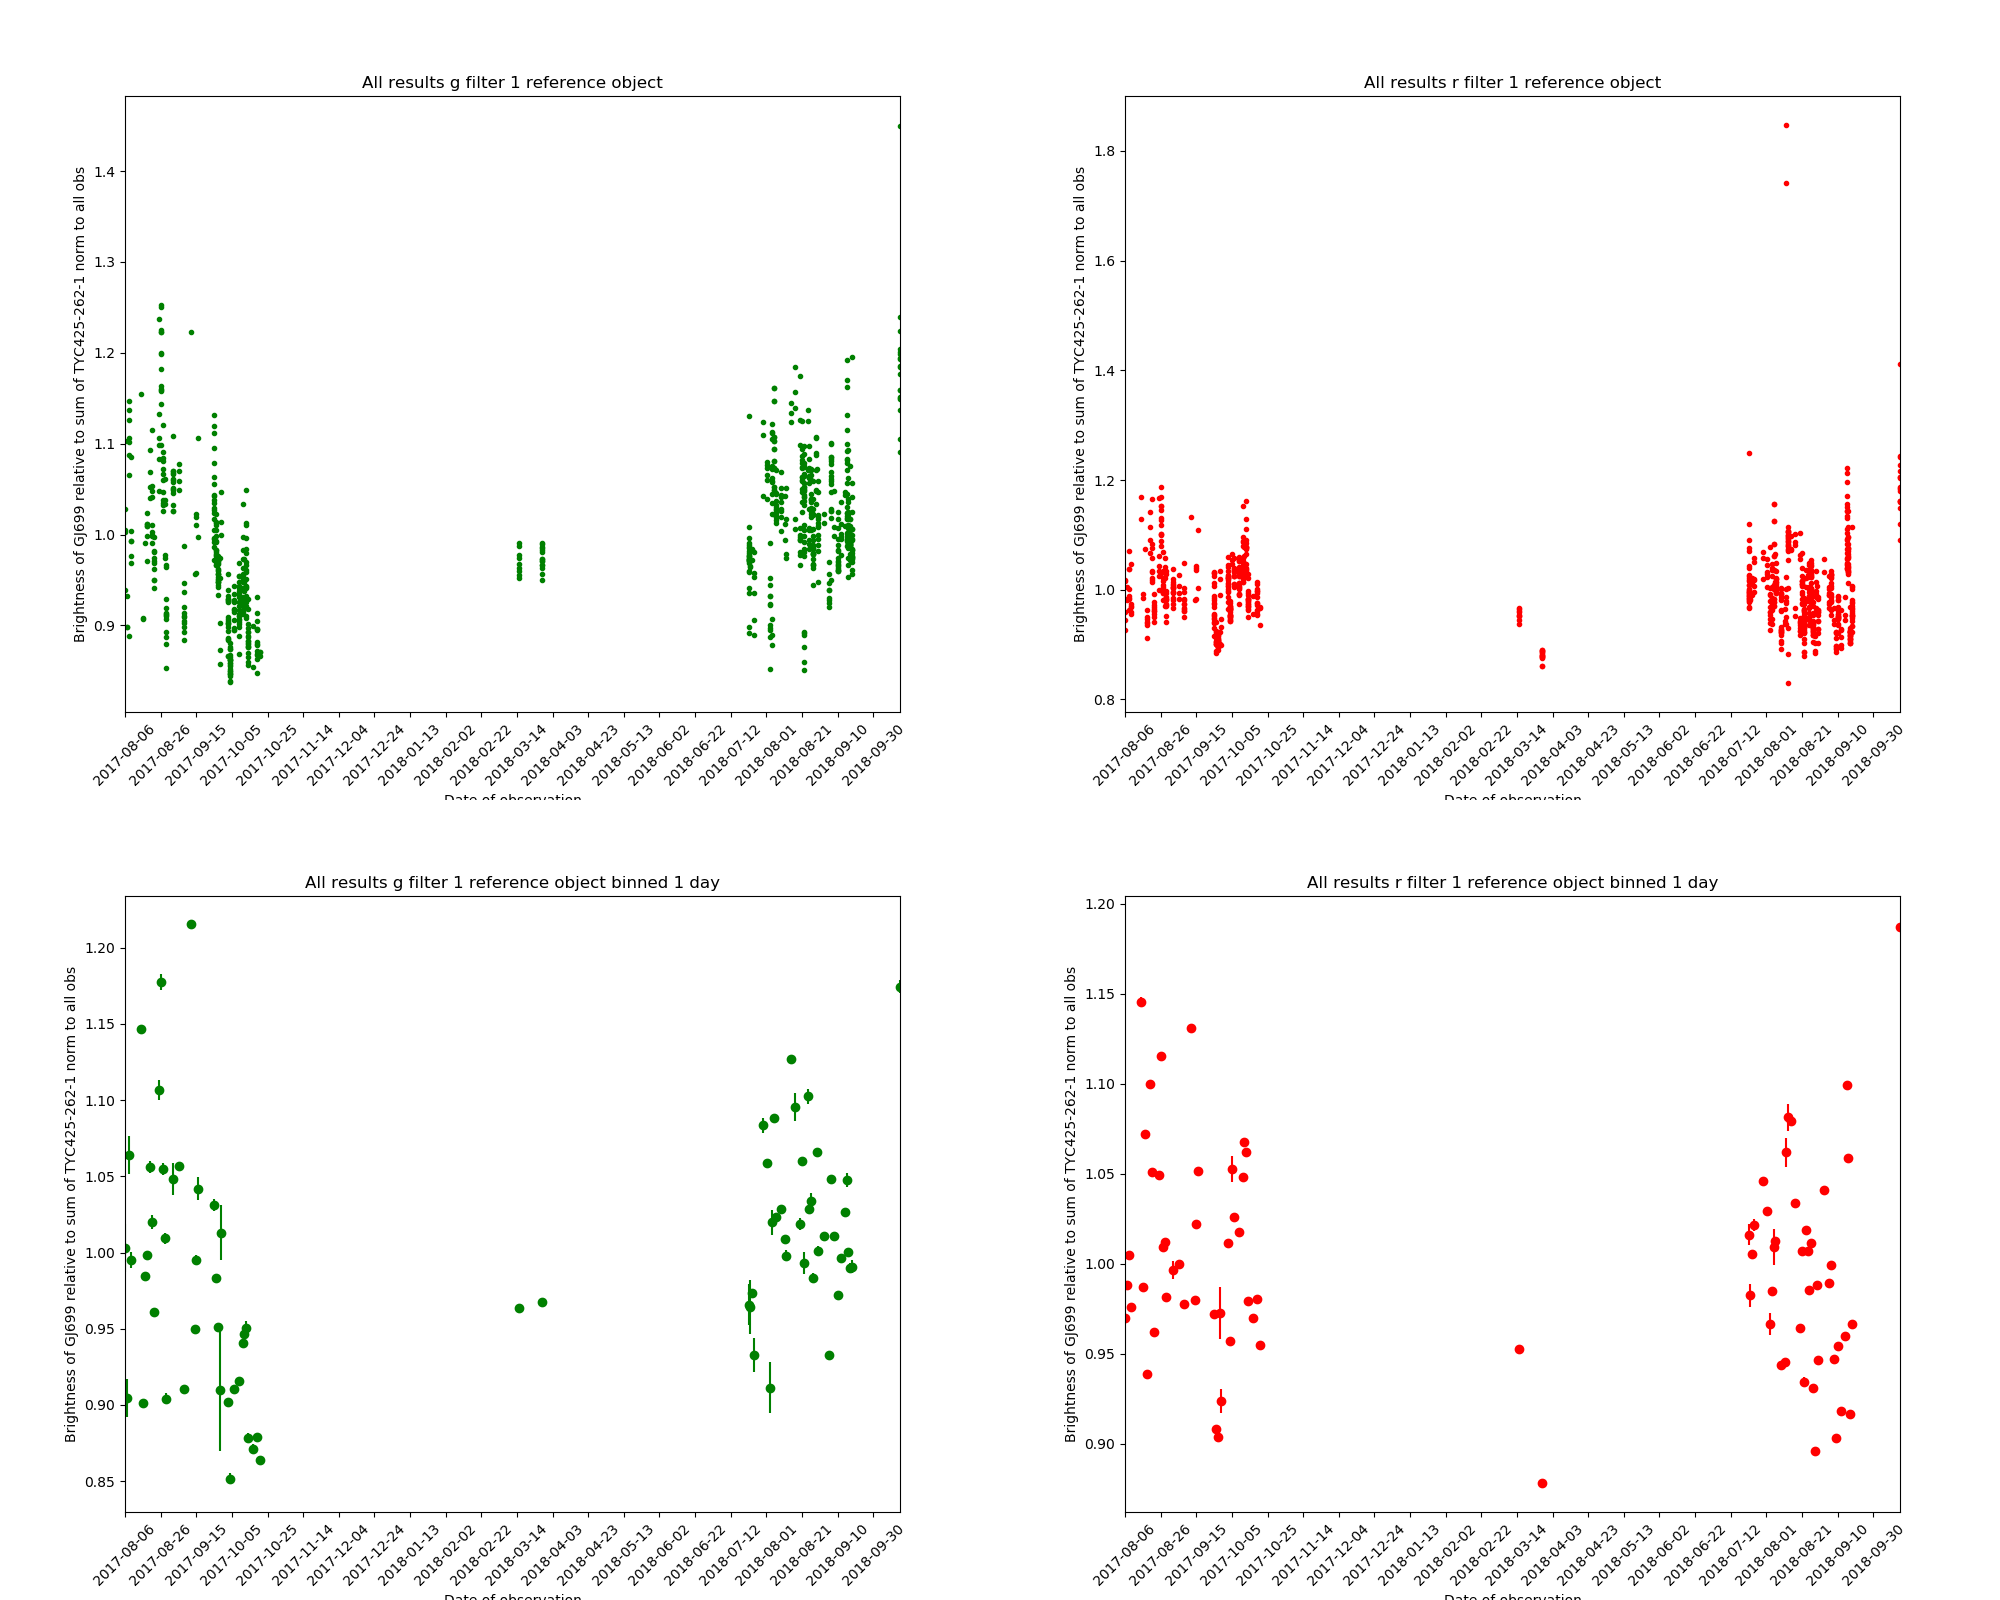
\includegraphics[scale=0.25]{images/allref1.png}
% \end{center}   
% \caption{This shows the ratio of the flux for the target, \bstar, to the strongest of the reference objects, TYC425-262-1.}
%   \protect\label{fig:allref1}
% \end{figure}
% 
% \begin{figure}[!htbp]
% \begin{center}
% 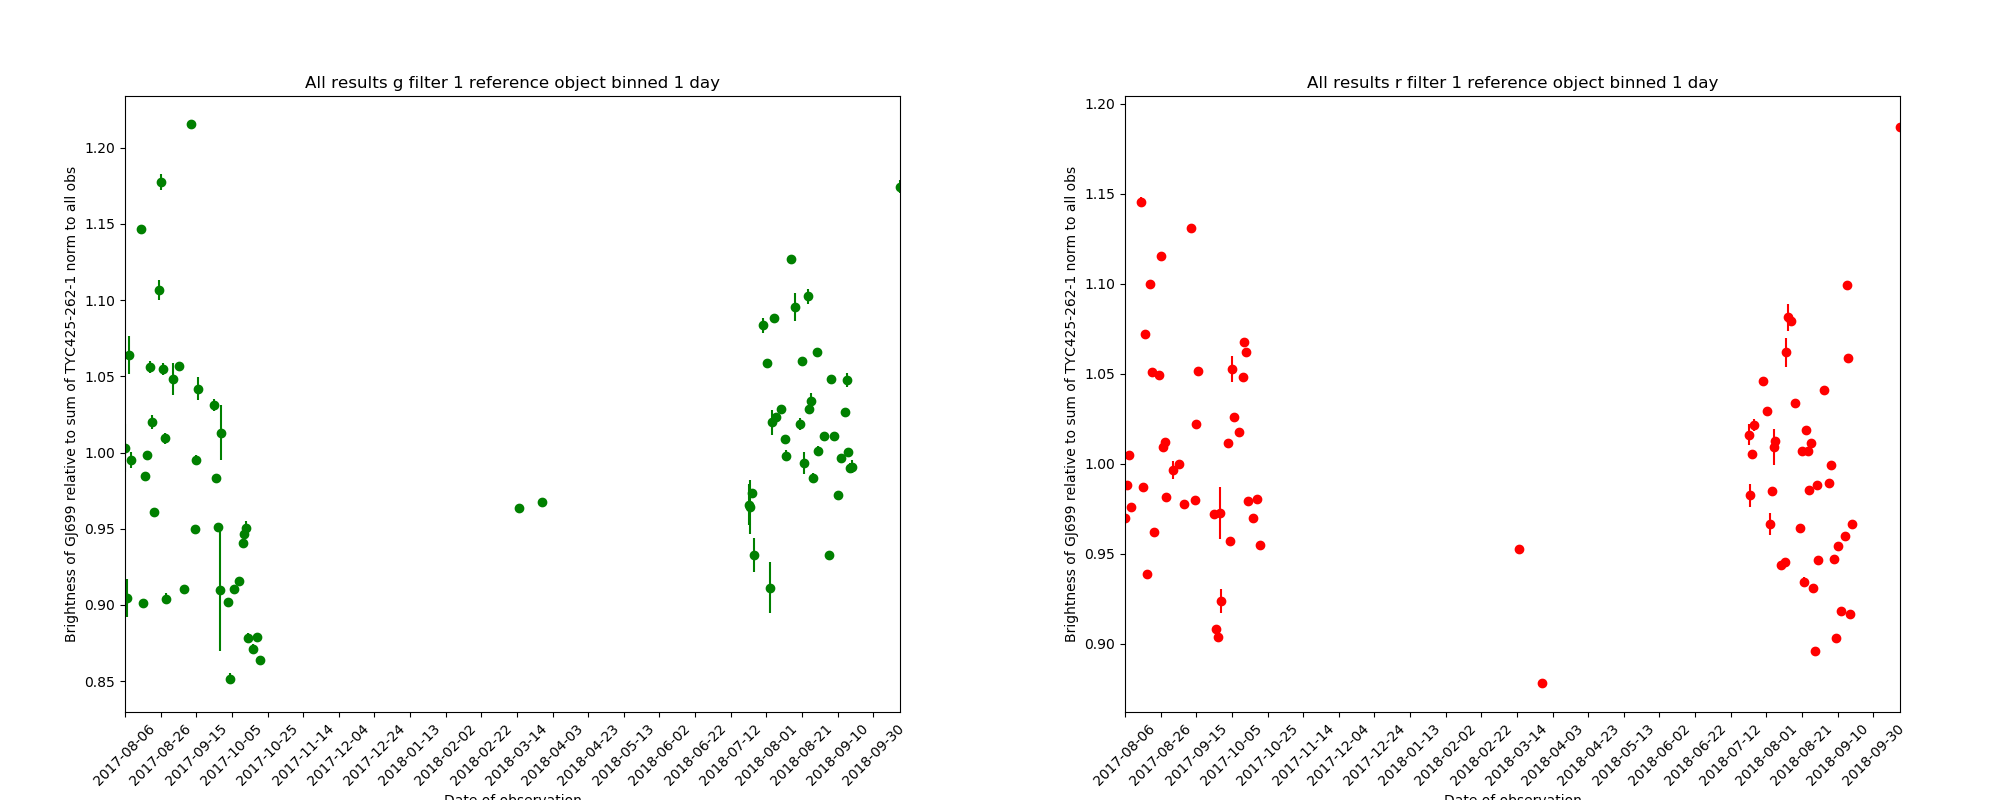
\includegraphics[scale=0.25]{images/allref1bin.png}
% \end{center}   
% \caption{This shows the ratio of the flux for the target, \bstar, to the strongest of the reference objects,
%   TYC425-262-1 per Fig. \ref{fig:allref1} and binned to 1 day.}
%   \protect\label{fig:allref1bin}
% \end{figure}
% 
% \begin{figure}[!htbp]
% \begin{center}
% 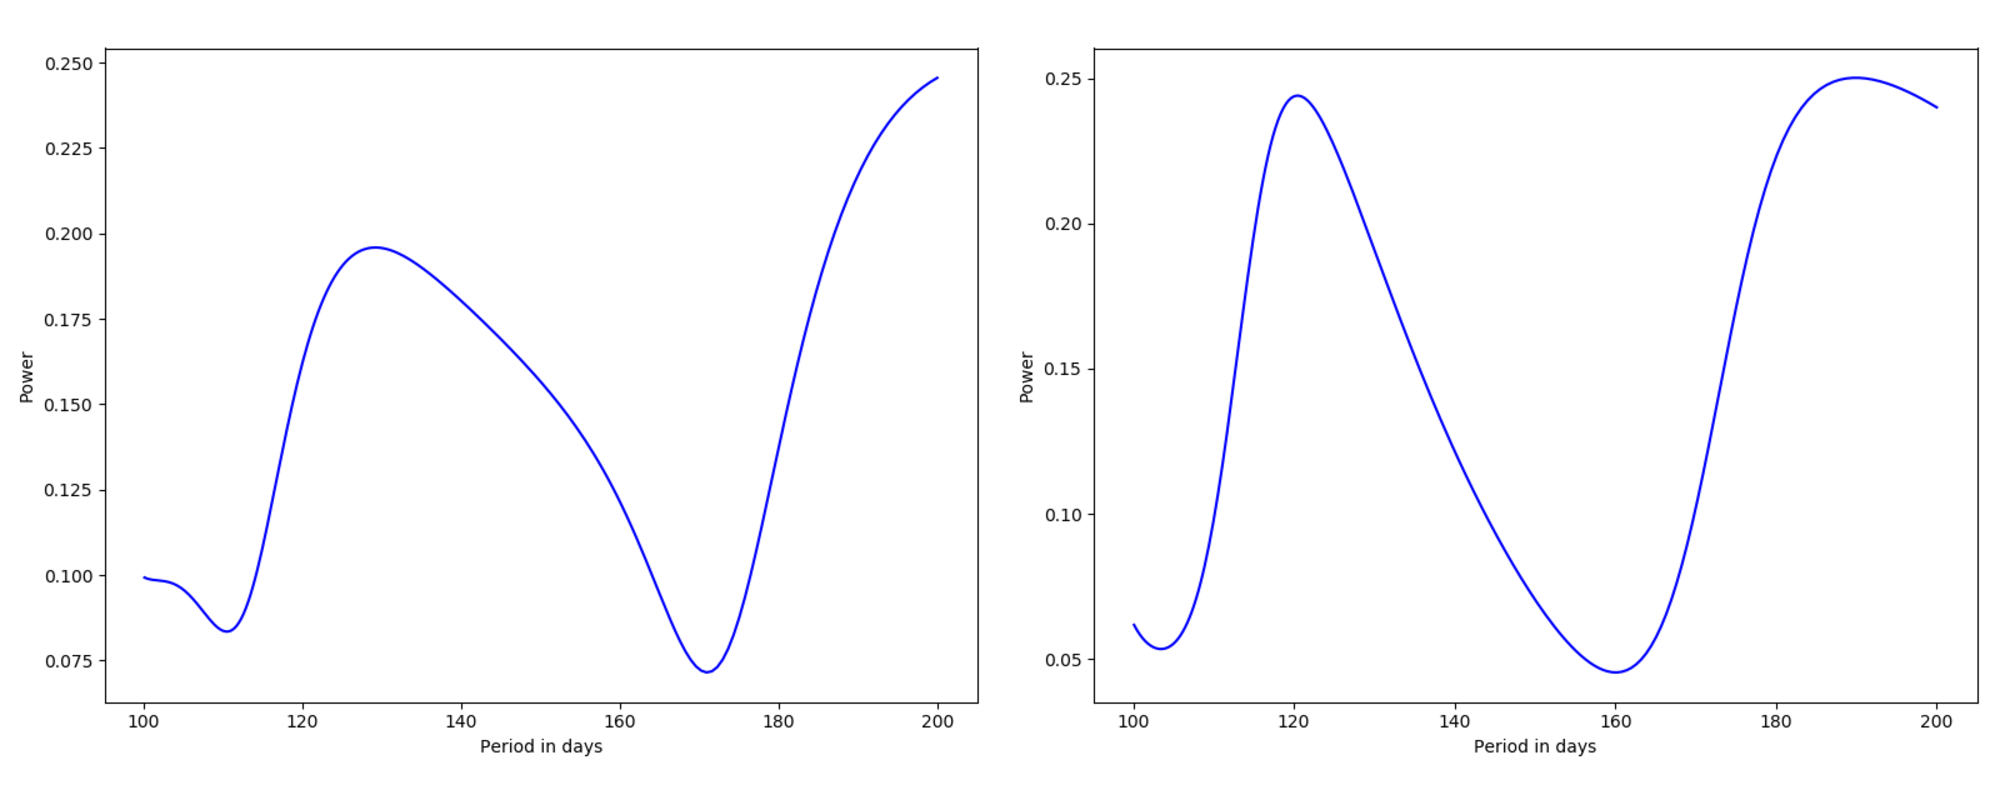
\includegraphics[scale=0.25]{images/ls1both.png}
% \end{center}   
% \caption{Periodograms obtained from Fig. \ref{fig:allref1}, left panel and Fig. \ref{fig:allref1bin} in right
%   panel. Only the \textbf{g} filter was used in this plot, the one from the \textbf{r} filter being almost identical.}
% \protect\label{fig:ls1both}
% \end{figure}
% \clearpage

